% Options for packages loaded elsewhere
\PassOptionsToPackage{unicode}{hyperref}
\PassOptionsToPackage{hyphens}{url}
%
\documentclass[
  letterpaper,
]{book}

\usepackage{amsmath,amssymb}
\usepackage{iftex}
\ifPDFTeX
  \usepackage[T1]{fontenc}
  \usepackage[utf8]{inputenc}
  \usepackage{textcomp} % provide euro and other symbols
\else % if luatex or xetex
  \usepackage{unicode-math}
  \defaultfontfeatures{Scale=MatchLowercase}
  \defaultfontfeatures[\rmfamily]{Ligatures=TeX,Scale=1}
\fi
\usepackage{lmodern}
\ifPDFTeX\else  
    % xetex/luatex font selection
\fi
% Use upquote if available, for straight quotes in verbatim environments
\IfFileExists{upquote.sty}{\usepackage{upquote}}{}
\IfFileExists{microtype.sty}{% use microtype if available
  \usepackage[]{microtype}
  \UseMicrotypeSet[protrusion]{basicmath} % disable protrusion for tt fonts
}{}
\makeatletter
\@ifundefined{KOMAClassName}{% if non-KOMA class
  \IfFileExists{parskip.sty}{%
    \usepackage{parskip}
  }{% else
    \setlength{\parindent}{0pt}
    \setlength{\parskip}{6pt plus 2pt minus 1pt}}
}{% if KOMA class
  \KOMAoptions{parskip=half}}
\makeatother
\usepackage{xcolor}
\usepackage{soul}
\setlength{\emergencystretch}{3em} % prevent overfull lines
\setcounter{secnumdepth}{5}
% Make \paragraph and \subparagraph free-standing
\ifx\paragraph\undefined\else
  \let\oldparagraph\paragraph
  \renewcommand{\paragraph}[1]{\oldparagraph{#1}\mbox{}}
\fi
\ifx\subparagraph\undefined\else
  \let\oldsubparagraph\subparagraph
  \renewcommand{\subparagraph}[1]{\oldsubparagraph{#1}\mbox{}}
\fi

\usepackage{color}
\usepackage{fancyvrb}
\newcommand{\VerbBar}{|}
\newcommand{\VERB}{\Verb[commandchars=\\\{\}]}
\DefineVerbatimEnvironment{Highlighting}{Verbatim}{commandchars=\\\{\}}
% Add ',fontsize=\small' for more characters per line
\usepackage{framed}
\definecolor{shadecolor}{RGB}{241,243,245}
\newenvironment{Shaded}{\begin{snugshade}}{\end{snugshade}}
\newcommand{\AlertTok}[1]{\textcolor[rgb]{0.68,0.00,0.00}{#1}}
\newcommand{\AnnotationTok}[1]{\textcolor[rgb]{0.37,0.37,0.37}{#1}}
\newcommand{\AttributeTok}[1]{\textcolor[rgb]{0.40,0.45,0.13}{#1}}
\newcommand{\BaseNTok}[1]{\textcolor[rgb]{0.68,0.00,0.00}{#1}}
\newcommand{\BuiltInTok}[1]{\textcolor[rgb]{0.00,0.23,0.31}{#1}}
\newcommand{\CharTok}[1]{\textcolor[rgb]{0.13,0.47,0.30}{#1}}
\newcommand{\CommentTok}[1]{\textcolor[rgb]{0.37,0.37,0.37}{#1}}
\newcommand{\CommentVarTok}[1]{\textcolor[rgb]{0.37,0.37,0.37}{\textit{#1}}}
\newcommand{\ConstantTok}[1]{\textcolor[rgb]{0.56,0.35,0.01}{#1}}
\newcommand{\ControlFlowTok}[1]{\textcolor[rgb]{0.00,0.23,0.31}{#1}}
\newcommand{\DataTypeTok}[1]{\textcolor[rgb]{0.68,0.00,0.00}{#1}}
\newcommand{\DecValTok}[1]{\textcolor[rgb]{0.68,0.00,0.00}{#1}}
\newcommand{\DocumentationTok}[1]{\textcolor[rgb]{0.37,0.37,0.37}{\textit{#1}}}
\newcommand{\ErrorTok}[1]{\textcolor[rgb]{0.68,0.00,0.00}{#1}}
\newcommand{\ExtensionTok}[1]{\textcolor[rgb]{0.00,0.23,0.31}{#1}}
\newcommand{\FloatTok}[1]{\textcolor[rgb]{0.68,0.00,0.00}{#1}}
\newcommand{\FunctionTok}[1]{\textcolor[rgb]{0.28,0.35,0.67}{#1}}
\newcommand{\ImportTok}[1]{\textcolor[rgb]{0.00,0.46,0.62}{#1}}
\newcommand{\InformationTok}[1]{\textcolor[rgb]{0.37,0.37,0.37}{#1}}
\newcommand{\KeywordTok}[1]{\textcolor[rgb]{0.00,0.23,0.31}{#1}}
\newcommand{\NormalTok}[1]{\textcolor[rgb]{0.00,0.23,0.31}{#1}}
\newcommand{\OperatorTok}[1]{\textcolor[rgb]{0.37,0.37,0.37}{#1}}
\newcommand{\OtherTok}[1]{\textcolor[rgb]{0.00,0.23,0.31}{#1}}
\newcommand{\PreprocessorTok}[1]{\textcolor[rgb]{0.68,0.00,0.00}{#1}}
\newcommand{\RegionMarkerTok}[1]{\textcolor[rgb]{0.00,0.23,0.31}{#1}}
\newcommand{\SpecialCharTok}[1]{\textcolor[rgb]{0.37,0.37,0.37}{#1}}
\newcommand{\SpecialStringTok}[1]{\textcolor[rgb]{0.13,0.47,0.30}{#1}}
\newcommand{\StringTok}[1]{\textcolor[rgb]{0.13,0.47,0.30}{#1}}
\newcommand{\VariableTok}[1]{\textcolor[rgb]{0.07,0.07,0.07}{#1}}
\newcommand{\VerbatimStringTok}[1]{\textcolor[rgb]{0.13,0.47,0.30}{#1}}
\newcommand{\WarningTok}[1]{\textcolor[rgb]{0.37,0.37,0.37}{\textit{#1}}}

\providecommand{\tightlist}{%
  \setlength{\itemsep}{0pt}\setlength{\parskip}{0pt}}\usepackage{longtable,booktabs,array}
\usepackage{calc} % for calculating minipage widths
% Correct order of tables after \paragraph or \subparagraph
\usepackage{etoolbox}
\makeatletter
\patchcmd\longtable{\par}{\if@noskipsec\mbox{}\fi\par}{}{}
\makeatother
% Allow footnotes in longtable head/foot
\IfFileExists{footnotehyper.sty}{\usepackage{footnotehyper}}{\usepackage{footnote}}
\makesavenoteenv{longtable}
\usepackage{graphicx}
\makeatletter
\def\maxwidth{\ifdim\Gin@nat@width>\linewidth\linewidth\else\Gin@nat@width\fi}
\def\maxheight{\ifdim\Gin@nat@height>\textheight\textheight\else\Gin@nat@height\fi}
\makeatother
% Scale images if necessary, so that they will not overflow the page
% margins by default, and it is still possible to overwrite the defaults
% using explicit options in \includegraphics[width, height, ...]{}
\setkeys{Gin}{width=\maxwidth,height=\maxheight,keepaspectratio}
% Set default figure placement to htbp
\makeatletter
\def\fps@figure{htbp}
\makeatother
\newlength{\cslhangindent}
\setlength{\cslhangindent}{1.5em}
\newlength{\csllabelwidth}
\setlength{\csllabelwidth}{3em}
\newlength{\cslentryspacingunit} % times entry-spacing
\setlength{\cslentryspacingunit}{\parskip}
\newenvironment{CSLReferences}[2] % #1 hanging-ident, #2 entry spacing
 {% don't indent paragraphs
  \setlength{\parindent}{0pt}
  % turn on hanging indent if param 1 is 1
  \ifodd #1
  \let\oldpar\par
  \def\par{\hangindent=\cslhangindent\oldpar}
  \fi
  % set entry spacing
  \setlength{\parskip}{#2\cslentryspacingunit}
 }%
 {}
\usepackage{calc}
\newcommand{\CSLBlock}[1]{#1\hfill\break}
\newcommand{\CSLLeftMargin}[1]{\parbox[t]{\csllabelwidth}{#1}}
\newcommand{\CSLRightInline}[1]{\parbox[t]{\linewidth - \csllabelwidth}{#1}\break}
\newcommand{\CSLIndent}[1]{\hspace{\cslhangindent}#1}

\makeatletter
\@ifpackageloaded{tcolorbox}{}{\usepackage[skins,breakable]{tcolorbox}}
\@ifpackageloaded{fontawesome5}{}{\usepackage{fontawesome5}}
\definecolor{quarto-callout-color}{HTML}{909090}
\definecolor{quarto-callout-note-color}{HTML}{0758E5}
\definecolor{quarto-callout-important-color}{HTML}{CC1914}
\definecolor{quarto-callout-warning-color}{HTML}{EB9113}
\definecolor{quarto-callout-tip-color}{HTML}{00A047}
\definecolor{quarto-callout-caution-color}{HTML}{FC5300}
\definecolor{quarto-callout-color-frame}{HTML}{acacac}
\definecolor{quarto-callout-note-color-frame}{HTML}{4582ec}
\definecolor{quarto-callout-important-color-frame}{HTML}{d9534f}
\definecolor{quarto-callout-warning-color-frame}{HTML}{f0ad4e}
\definecolor{quarto-callout-tip-color-frame}{HTML}{02b875}
\definecolor{quarto-callout-caution-color-frame}{HTML}{fd7e14}
\makeatother
\makeatletter
\makeatother
\makeatletter
\@ifpackageloaded{bookmark}{}{\usepackage{bookmark}}
\makeatother
\makeatletter
\@ifpackageloaded{caption}{}{\usepackage{caption}}
\AtBeginDocument{%
\ifdefined\contentsname
  \renewcommand*\contentsname{Table of contents}
\else
  \newcommand\contentsname{Table of contents}
\fi
\ifdefined\listfigurename
  \renewcommand*\listfigurename{List of Figures}
\else
  \newcommand\listfigurename{List of Figures}
\fi
\ifdefined\listtablename
  \renewcommand*\listtablename{List of Tables}
\else
  \newcommand\listtablename{List of Tables}
\fi
\ifdefined\figurename
  \renewcommand*\figurename{Figure}
\else
  \newcommand\figurename{Figure}
\fi
\ifdefined\tablename
  \renewcommand*\tablename{Table}
\else
  \newcommand\tablename{Table}
\fi
}
\@ifpackageloaded{float}{}{\usepackage{float}}
\floatstyle{ruled}
\@ifundefined{c@chapter}{\newfloat{codelisting}{h}{lop}}{\newfloat{codelisting}{h}{lop}[chapter]}
\floatname{codelisting}{Listing}
\newcommand*\listoflistings{\listof{codelisting}{List of Listings}}
\makeatother
\makeatletter
\@ifpackageloaded{caption}{}{\usepackage{caption}}
\@ifpackageloaded{subcaption}{}{\usepackage{subcaption}}
\makeatother
\makeatletter
\@ifpackageloaded{tcolorbox}{}{\usepackage[skins,breakable]{tcolorbox}}
\makeatother
\makeatletter
\@ifundefined{shadecolor}{\definecolor{shadecolor}{rgb}{.97, .97, .97}}
\makeatother
\makeatletter
\makeatother
\makeatletter
\makeatother
\ifLuaTeX
  \usepackage{selnolig}  % disable illegal ligatures
\fi
\IfFileExists{bookmark.sty}{\usepackage{bookmark}}{\usepackage{hyperref}}
\IfFileExists{xurl.sty}{\usepackage{xurl}}{} % add URL line breaks if available
\urlstyle{same} % disable monospaced font for URLs
\hypersetup{
  pdftitle={Statistical Programming for the Social Sciences Using R},
  pdfauthor={Wesley Stubenbord},
  hidelinks,
  pdfcreator={LaTeX via pandoc}}

\title{Statistical Programming for the Social Sciences Using R}
\author{Wesley Stubenbord}
\date{10 April 2024}

\begin{document}
\frontmatter
\maketitle
\ifdefined\Shaded\renewenvironment{Shaded}{\begin{tcolorbox}[boxrule=0pt, borderline west={3pt}{0pt}{shadecolor}, interior hidden, breakable, enhanced, sharp corners, frame hidden]}{\end{tcolorbox}}\fi

\renewcommand*\contentsname{Table of contents}
{
\setcounter{tocdepth}{2}
\tableofcontents
}
\mainmatter
\bookmarksetup{startatroot}

\hypertarget{preface}{%
\chapter*{Preface}\label{preface}}
\addcontentsline{toc}{chapter}{Preface}

\markboth{Preface}{Preface}

Welcome! This is the companion website for \emph{Statistical Programming
for the Social Sciences Using R}, taught at the Sciences Po Reims campus
in the Spring 2024 term. The course is a broad introduction to the
general programming skills required for data analysis in the social
sciences.

This online textbook contains the relevant tutorials for each week's
lesson as well as other resources that you may find helpful throughout
the course. The syllabus, slides, assignment submission portals, and
other files can be found on the
\href{https://moodle.sciences-po.fr/course/view.php?id=40782}{course
Moodle site}.

\hypertarget{resources}{%
\section*{Resources}\label{resources}}
\addcontentsline{toc}{section}{Resources}

\markright{Resources}

There are a variety of \texttt{R} resources out there, many of which
have been useful in developing this course.

If you would like to dig deeper into a particular topic or simply want
to read other explanations of the concepts discussed in this course,
here is a list of helpful resources:

\begin{itemize}
\tightlist
\item
  \textbf{\emph{R for Data Science, 2e}} by Hadley Wickham, Mine
  Çetinkaya-Rundel, and Garrett Grolemund
  (\href{https://r4ds.hadley.nz/}{link}): A free introductory textbook
  on how to use the many features of \texttt{R} to make sense of data,
  co-authored by the creator of the tidyverse package.
\item
  \textbf{\emph{Data Visualization}} by Kieran Healy
  (\href{https://socviz.co/}{draft textbook}): An introductory textbook
  on how to make practical and beautiful data visualizations in
  \texttt{R}. Healy has a distinctive and appealing visual style. He
  also happens to be an accomplished sociologist, known especially for
  his
  \href{https://kieranhealy.org/files/papers/fuck-nuance.pdf}{disdain of
  nuanced theory} and his
  \href{https://kieranhealy.org/publications/}{broader contributions} to
  the study of morals and markets. His examples are especially relevant
  to the social sciences as a result.
\item
  \textbf{\emph{Introduction to Econometrics with R}} by Florian Oswald
  and colleagues at Sciences Po
  (\href{https://scpoecon.github.io/ScPoEconometrics/index.html}{companion
  textbook} and
  \href{https://github.com/ScPoEcon/ScPoEconometrics-Slides}{slides}):
  you may very well be taking this course because you couldn't get into
  this other course. For this, I am both sorry, because you are missing
  out, and not sorry, because it keeps me gainfully employed and gives
  me an excuse to write this textbook. Fortunately for you, the course
  developed by Professor Oswald and colleagues is freely-available
  online. If you'd like to see material which is more heavily-weighted
  towards applied statistical methods (especially applied economics),
  take a look at their extremely well put together course. You may very
  well rue the day you woke up late for course sign-ups.
\item
  \textbf{ggplot2: Elegant Graphics for Data Analysis (3e)} by Hadley
  Wickham, Danielle Navarro, and Thomas Lin Pedersen
  (\href{https://ggplot2-book.org/}{link}): An in-depth explanation of
  how the popular \texttt{ggplot2} data visualization package works.
\end{itemize}

\hypertarget{change-log}{%
\section*{Change Log}\label{change-log}}
\addcontentsline{toc}{section}{Change Log}

\markright{Change Log}

I'll be making frequent updates to the textbook, often changing the
appearance, structure, and/or content. In general, these changes won't
be substantive. In other words, they won't change what you are required
to know or how you are expected to do things. You might, however, find
that certain sections become more detailed as the course progresses. If
you would like to see a detailed list of changes (including my frequent
struggles with word choice), take a look at the
\href{https://github.com/wstubenbord/ScPoSPSSUR}{GitHub repository}. For
those of you with better things to do in your spare time, a brief
chronological summary of updates is provided below:

\begin{itemize}
\tightlist
\item
  \textbf{2024.04.09} - Minor edits to Chapter 8.
\item
  \textbf{2024.04.08} - Chapter 8 has been posted.
\item
  \textbf{2024.03.26} - Minor edits to Chapter 7.
\item
  \textbf{2024.03.25} - Chapter 7 has been posted.
\item
  \textbf{2024.03.19} - Minor edits to Chapter 6.
\item
  \textbf{2024.03.17} - Chapter 6 has been posted.
\item
  \textbf{2024.03.07} - More minor edits to Chapter 5.
\item
  \textbf{2024.03.06} - Minor edits to Chapter 5 for clarity, typos.
\item
  \textbf{2024.03.05} - Homework 3 has been posted.
\item
  \textbf{2024.03.03} - Chapter 5 has been posted.
\item
  \textbf{2024.03.01} - Fixes to Chapter 4 code. A couple of functions
  were missing \texttt{scales::}.
\item
  \textbf{2024.02.25} - Chapter 4 has been posted.
\item
  \textbf{2024.02.22} - Another resource added to the preface. Minor
  copy edits.
\item
  \textbf{2024.02.18} - I've refactored the course website from R
  Markdown to Quarto. You may notice some significant changes to the
  appearance of the website, including the appearance of a new
  navigation bar on the right-hand side (used for navigating sections
  within a chapter) and changes to the standard navigation bar on the
  left-hand side (no more sections and subsections). I'm not completely
  in love the navigation bar changes, but the other benefits of
  switching to Quarto are worth it (more functionality, better visual
  appeal in other areas). Links have been updated as a result (apologies
  to those of you who may have bookmarked sections). Also, a technical
  note has been added to Homework \#2 (it will not affect the grading of
  relevant questions).
\end{itemize}

\bookmarksetup{startatroot}

\hypertarget{an-introduction-to-r}{%
\chapter{\texorpdfstring{An Introduction to
\texttt{R}}{An Introduction to R}}\label{an-introduction-to-r}}

If you are taking this course, you probably don't need an explanation of
why \texttt{R} is useful or why it may be in your best interest to take
this course. So I won't beleaguer the point: yes, \texttt{R} will make
you fabulously rich; yes, it will help you make new friends; and yes, it
will allow you to escape your own mortality. Or, at the very least, it
will allow you to do some interesting things with data, which is nearly
as nice.

Let's jump into it then. To get started with \texttt{R}, you will need
to install two things:

\begin{enumerate}
\def\labelenumi{\arabic{enumi}.}
\item
  \textbf{\texttt{R}}, a programming language
\item
  \textbf{RStudio}, a software program that helps you program in
  \texttt{R}

  \begin{itemize}
  \tightlist
  \item
    This type of software program is known as an Integrated Development
    Environment (IDE)
  \end{itemize}
\end{enumerate}

Truth be told, you don't really need RStudio to program in \texttt{R},
but it certainly makes life easier. The difference between programming
in \texttt{R} and programming in \texttt{R} using RStudio might be akin
to the difference between driving a Fiat Panda and driving a Ferrari.
Both will get you to the same place, but one is more likely to be an
enjoyable experience. We will be using RStudio throughout the rest of
this journey as a result.

\hypertarget{installing-r}{%
\section{\texorpdfstring{Installing
\texttt{R}}{Installing R}}\label{installing-r}}

To install \texttt{R}, go to \url{https://cran.irsn.fr/index.html},
select the appropriate operating system, and follow the instructions.
For example, if you have a Mac, you will click on ``Download R for
macOS,'' followed by the ``R-4.3.2-arm64.pkg'' link beneath the ``Latest
release'' header. If you have a PC running Windows, you will click on
``Download R for Windows'' followed by ``install R for the first time''
then ``Download R-4.3.2 for Windows.''

In either case, your browser will start downloading an executable
installation file which you will then need to run to install \texttt{R}.

\begin{tcolorbox}[enhanced jigsaw, colframe=quarto-callout-caution-color-frame, colback=white, title=\textcolor{quarto-callout-caution-color}{\faFire}\hspace{0.5em}{Caution}, opacitybacktitle=0.6, coltitle=black, colbacktitle=quarto-callout-caution-color!10!white, arc=.35mm, leftrule=.75mm, bottomtitle=1mm, bottomrule=.15mm, breakable, opacityback=0, titlerule=0mm, rightrule=.15mm, left=2mm, toptitle=1mm, toprule=.15mm]

A couple of things you may need to watch out for:

\begin{itemize}
\item
  If you are using an older laptop (\textgreater10 years old), you may
  need to download a different version of \texttt{R} or RStudio. If in
  doubt, read the instructions on the download page and refer to your
  operating system version to find the right version.
\item
  If you have very little hard drive space on your computer, you may
  need to clear some space before you install RStudio. The latest
  RStudio version requires 215 MB and you will likely need some
  additional space for other software and data we will be using in the
  course later on. Around 2 GB should suffice.
\end{itemize}

\end{tcolorbox}

\hypertarget{installing-rstudio}{%
\section{Installing RStudio}\label{installing-rstudio}}

Once you've installed \texttt{R}, go to
\url{https://posit.co/download/rstudio-desktop/}.

Posit (a company formerly known as RStudio) offers \textbf{RStudio
Desktop} free of charge. Posit also offers a cloud-hosted version of the
software (called Posit Cloud) which has both free and paid tiers. If you
have trouble running RStudio Desktop on your computer, you may wish to
consider using a Posit Cloud account, as described in the course
syllabus.

When you've click on the link above, you'll find that you are ahead of
the game. Step 1 is complete, you've already installed \texttt{R}. Here
you'll find different versions of RStudio according to your computer's
operating system. Select the operating system that corresponds to your
particular case (Windows, MacOS, or Linux), download the installer, and
then run the installation file from your computer. Next, follow the
on-screen steps to complete the set-up.

If all goes well, your screen should look something like this once you
have RStudio correctly installed and running:

\includegraphics{images/RStudio clean install.png}

If your screen looks more like the image below, it means that you've
accidentally opened RGui, a basic graphical user interface included with
\texttt{R}, and not RStudio. We're always going to be working with
RStudio for this class, so close out of RGui and open RStudio instead.

\includegraphics{images/Base R GUI.PNG}

\hypertarget{using-the-console}{%
\section{Using the Console}\label{using-the-console}}

Now the fun begins. The RStudio window you've opened consists of a few
different parts. The most important of these right now is the console
\href{https://docs.posit.co/ide/user/ide/guide/ui/ui-panes.html}{pane}
(highlighted with a black square below).

\includegraphics{images/RStudio console box.png}

The console allows you to interact with your computer using \texttt{R}.
So, for example, if you want to use your computer as an over-sized
calculator, you can type the following \texttt{R} code in the console:

\begin{Shaded}
\begin{Highlighting}[]
\DecValTok{1} \SpecialCharTok{+} \DecValTok{1}
\end{Highlighting}
\end{Shaded}

What happens when you press \texttt{Enter} on your keyboard? You get
something like this:

\begin{Shaded}
\begin{Highlighting}[]
\DecValTok{1} \SpecialCharTok{+} \DecValTok{1}
\end{Highlighting}
\end{Shaded}

\begin{verbatim}
[1] 2
\end{verbatim}

You've provided an \textbf{input}, \texttt{1+1}, and received an
\textbf{output}, \texttt{2}. In other words, using the language of
\texttt{R}, you've told your computer to add one plus one and your
computer has correctly interpreted your command and \emph{returned} (or
output) an answer, two. When your computer does not know how to
interpret a command, usually because you've made a mistake, you will
receive an error message as the output instead. Identifying errors and
being able to correct them is an essential skill for a programmer and
one we will practice, often accidentally, throughout the course.

One more note about outputs: the first number in brackets next to your
output, \texttt{{[}1{]}}, indicates the index number of the
output.\footnote{In \texttt{R}, unlike in other programming languages,
  the first value in any data structure (e.g., a vector) has an index
  number of \texttt{1} rather than \texttt{0}. This makes intuitive
  sense. If you were asked to count people in line at a boulangerie, you
  would call the next person waiting to place their order the
  \emph{first} person in line, not the \emph{zero}eth. In Python, you
  would call them the \emph{zero}eth person and they would have an index
  number of \texttt{0} instead of \texttt{1}. For more on where this
  comes from, see
  \href{https://en.wikipedia.org/wiki/Zero-based_numbering}{here}.} This
is especially helpful when you are running code that generates multiple
outputs. See below, for example, where we input \texttt{LETTERS} and
receive a list of letters in the English alphabet as the output (note,
``T'' is the 20th letter and our 20th output).

\begin{Shaded}
\begin{Highlighting}[]
\NormalTok{LETTERS}
\end{Highlighting}
\end{Shaded}

\begin{verbatim}
 [1] "A" "B" "C" "D" "E" "F" "G" "H" "I" "J" "K" "L" "M" "N" "O" "P" "Q" "R" "S"
[20] "T" "U" "V" "W" "X" "Y" "Z"
\end{verbatim}

Try entering a few more inputs in the console:

\begin{enumerate}
\def\labelenumi{\arabic{enumi}.}
\item
  \texttt{10/3}
\item
  \texttt{(10/3)\ +\ 1}
\item
  \texttt{(10/3)\ +\ 1\ +\ (5.111)\textbackslash{}\^{}2}
\end{enumerate}

As you can see, \texttt{R} is able to handle basic math operations with
ease. What about other operations? Can you work with variables in
\texttt{R}, for example?

Try typing this in the console:

\begin{Shaded}
\begin{Highlighting}[]
\NormalTok{x }\OtherTok{=} \DecValTok{1}
\end{Highlighting}
\end{Shaded}

What happens when you press \texttt{Enter}?

\includegraphics{images/RStudio console_x1.png}

Unlike before, there is no output when you press \texttt{Enter}. But,
that doesn't mean nothing happened. In fact, something has happened.
You've stored a value, \texttt{1}, in a variable, \texttt{x}, somewhere
in your computer's memory or in what we might call the
\textbf{environment}. You don't receive an output, but RStudio reminds
you of your new object's existence via the environment pane in the top
right.

We can recall the value we input into our variable, \texttt{x}, by
entering the object name in the console:

\begin{Shaded}
\begin{Highlighting}[]
\NormalTok{x}
\end{Highlighting}
\end{Shaded}

\begin{verbatim}
[1] 1
\end{verbatim}

See! Your computer remembers what you stored in the environment.

Try the following on your own in the console and then take a look at the
answer:

\begin{enumerate}
\def\labelenumi{\arabic{enumi}.}
\item
  Can you assign a new value to your variable, \texttt{x}?

  \begin{tcolorbox}[enhanced jigsaw, colframe=quarto-callout-tip-color-frame, colback=white, title=\textcolor{quarto-callout-tip-color}{\faLightbulb}\hspace{0.5em}{Answer}, opacitybacktitle=0.6, coltitle=black, colbacktitle=quarto-callout-tip-color!10!white, arc=.35mm, leftrule=.75mm, bottomtitle=1mm, bottomrule=.15mm, breakable, opacityback=0, titlerule=0mm, rightrule=.15mm, left=2mm, toptitle=1mm, toprule=.15mm]

  Yes!

\begin{Shaded}
\begin{Highlighting}[]
\NormalTok{x }\OtherTok{=} \DecValTok{3}
\NormalTok{x}
\end{Highlighting}
\end{Shaded}

\begin{verbatim}
[1] 3
\end{verbatim}

  \end{tcolorbox}
\item
  Can you perform math operations on a variable (e.g., \texttt{x*5})?

  \begin{tcolorbox}[enhanced jigsaw, colframe=quarto-callout-tip-color-frame, colback=white, title=\textcolor{quarto-callout-tip-color}{\faLightbulb}\hspace{0.5em}{Answer}, opacitybacktitle=0.6, coltitle=black, colbacktitle=quarto-callout-tip-color!10!white, arc=.35mm, leftrule=.75mm, bottomtitle=1mm, bottomrule=.15mm, breakable, opacityback=0, titlerule=0mm, rightrule=.15mm, left=2mm, toptitle=1mm, toprule=.15mm]

  Yes!

\begin{Shaded}
\begin{Highlighting}[]
\NormalTok{x }\SpecialCharTok{*} \DecValTok{5}
\end{Highlighting}
\end{Shaded}

\begin{verbatim}
[1] 15
\end{verbatim}

  \end{tcolorbox}
\item
  Can you create a new variable, \texttt{y}, and use it in math
  operations with \texttt{x} (e.g., \texttt{x\ *\ y})?

  \begin{tcolorbox}[enhanced jigsaw, colframe=quarto-callout-tip-color-frame, colback=white, title=\textcolor{quarto-callout-tip-color}{\faLightbulb}\hspace{0.5em}{Answer}, opacitybacktitle=0.6, coltitle=black, colbacktitle=quarto-callout-tip-color!10!white, arc=.35mm, leftrule=.75mm, bottomtitle=1mm, bottomrule=.15mm, breakable, opacityback=0, titlerule=0mm, rightrule=.15mm, left=2mm, toptitle=1mm, toprule=.15mm]

  Yes!

\begin{Shaded}
\begin{Highlighting}[]
\NormalTok{y }\OtherTok{=} \DecValTok{2}
\NormalTok{x }\SpecialCharTok{*}\NormalTok{ y}
\end{Highlighting}
\end{Shaded}

\begin{verbatim}
[1] 6
\end{verbatim}

  \end{tcolorbox}
\item
  Can you change the type of variable? What if, for example, I want
  \texttt{x} to be equal to the word \texttt{"apple"} instead?

  \begin{tcolorbox}[enhanced jigsaw, colframe=quarto-callout-tip-color-frame, colback=white, title=\textcolor{quarto-callout-tip-color}{\faLightbulb}\hspace{0.5em}{Answer}, opacitybacktitle=0.6, coltitle=black, colbacktitle=quarto-callout-tip-color!10!white, arc=.35mm, leftrule=.75mm, bottomtitle=1mm, bottomrule=.15mm, breakable, opacityback=0, titlerule=0mm, rightrule=.15mm, left=2mm, toptitle=1mm, toprule=.15mm]

  Yes! For letters and words, you just have to use quotation marks:

\begin{Shaded}
\begin{Highlighting}[]
\NormalTok{x }\OtherTok{=} \StringTok{"apple"}
\NormalTok{x}
\end{Highlighting}
\end{Shaded}

\begin{verbatim}
[1] "apple"
\end{verbatim}

  \end{tcolorbox}
\end{enumerate}

\hypertarget{calculations-with-objects}{%
\section{Calculations with Objects}\label{calculations-with-objects}}

If you've made it this far, well done! Here's something else you can
try. Enter the following in the console:

\begin{Shaded}
\begin{Highlighting}[]
\NormalTok{x }\OtherTok{\textless{}{-}} \FunctionTok{c}\NormalTok{(}\DecValTok{1}\NormalTok{, }\DecValTok{2}\NormalTok{, }\DecValTok{3}\NormalTok{, }\DecValTok{4}\NormalTok{, }\DecValTok{5}\NormalTok{)}
\end{Highlighting}
\end{Shaded}

You'll notice that we're using a different operator here. It's a less
than symbol, \texttt{\textless{}}, followed by a dash, \texttt{-}. This
is called an \textbf{assignment operator} and it has the same function
as the equals sign, \texttt{=}. You can use either, but sticking with
\texttt{\textless{}-} when assigning values to objects will make life
easier later on.

What happens when you press \texttt{Enter}? You have created a
\textbf{vector}. In \texttt{R}, a vector is an \textbf{object} that
holds a set of values of the same type. In this case, the vector
\texttt{x} contains a set of numbers: \(\{1,2,3,4,5\}\). You can think
of an object as a container which holds things and a ``variable'' as the
name we use to refer to a specific object. Here, \texttt{x} is the
variable name we've given to our vector of numbers, which is an object.
Most things in \texttt{R} are objects.

We can do all sorts of things with vectors and other objects in
\texttt{R}. We can, for example, find the sum of a vector.

\begin{Shaded}
\begin{Highlighting}[]
\FunctionTok{sum}\NormalTok{(x)}
\end{Highlighting}
\end{Shaded}

\begin{verbatim}
[1] 15
\end{verbatim}

How did we get an output of 15? We summed each of the elements of our
vector \texttt{x}: \(1+2+3+4+5 = 15\). We can also find the mean of a
vector:

\begin{Shaded}
\begin{Highlighting}[]
\FunctionTok{mean}\NormalTok{(x)}
\end{Highlighting}
\end{Shaded}

\begin{verbatim}
[1] 3
\end{verbatim}

And, we can perform other operations on vectors too. Try each of the
following questions on your own in the console and then click on the
answer to check your work:

\begin{enumerate}
\def\labelenumi{\arabic{enumi}.}
\item
  Can you find the median of a vector?

  \begin{tcolorbox}[enhanced jigsaw, colframe=quarto-callout-tip-color-frame, colback=white, title=\textcolor{quarto-callout-tip-color}{\faLightbulb}\hspace{0.5em}{Answer}, opacitybacktitle=0.6, coltitle=black, colbacktitle=quarto-callout-tip-color!10!white, arc=.35mm, leftrule=.75mm, bottomtitle=1mm, bottomrule=.15mm, breakable, opacityback=0, titlerule=0mm, rightrule=.15mm, left=2mm, toptitle=1mm, toprule=.15mm]

  You can use \texttt{median()} instead of \texttt{mean()}!

\begin{Shaded}
\begin{Highlighting}[]
\FunctionTok{median}\NormalTok{(x)}
\end{Highlighting}
\end{Shaded}

\begin{verbatim}
[1] 3
\end{verbatim}

  Some functions are easy to guess, like \texttt{median()}, but others
  are false cognates just like in human languages (e.g., \texttt{mode()}
  won't get you what you might expect in \texttt{R} and asking for
  \emph{pain} in English won't get you
  \href{https://fr.wikipedia.org/wiki/Pain}{bread}). We'll talk more
  about functions and how to figure out what they do in the next
  chapter.

  \end{tcolorbox}
\item
  What happens when you multiply a vector by a number?

  \begin{tcolorbox}[enhanced jigsaw, colframe=quarto-callout-tip-color-frame, colback=white, title=\textcolor{quarto-callout-tip-color}{\faLightbulb}\hspace{0.5em}{Answer}, opacitybacktitle=0.6, coltitle=black, colbacktitle=quarto-callout-tip-color!10!white, arc=.35mm, leftrule=.75mm, bottomtitle=1mm, bottomrule=.15mm, breakable, opacityback=0, titlerule=0mm, rightrule=.15mm, left=2mm, toptitle=1mm, toprule=.15mm]

  Each value in the vector is multiplied by that number!

\begin{Shaded}
\begin{Highlighting}[]
\NormalTok{x }\SpecialCharTok{*} \DecValTok{2}
\end{Highlighting}
\end{Shaded}

\begin{verbatim}
[1]  2  4  6  8 10
\end{verbatim}

  \end{tcolorbox}
\item
  Can you create a new vector which consists only of letters? What about
  words?

  \begin{tcolorbox}[enhanced jigsaw, colframe=quarto-callout-tip-color-frame, colback=white, title=\textcolor{quarto-callout-tip-color}{\faLightbulb}\hspace{0.5em}{Answer}, opacitybacktitle=0.6, coltitle=black, colbacktitle=quarto-callout-tip-color!10!white, arc=.35mm, leftrule=.75mm, bottomtitle=1mm, bottomrule=.15mm, breakable, opacityback=0, titlerule=0mm, rightrule=.15mm, left=2mm, toptitle=1mm, toprule=.15mm]

  Yes! Instead of using numbers, you can create a vector using letters
  enclosed in quotation marks.

\begin{Shaded}
\begin{Highlighting}[]
\NormalTok{y }\OtherTok{\textless{}{-}} \FunctionTok{c}\NormalTok{(}\StringTok{\textquotesingle{}a\textquotesingle{}}\NormalTok{, }\StringTok{\textquotesingle{}b\textquotesingle{}}\NormalTok{, }\StringTok{\textquotesingle{}c\textquotesingle{}}\NormalTok{)}
\NormalTok{y}
\end{Highlighting}
\end{Shaded}

\begin{verbatim}
[1] "a" "b" "c"
\end{verbatim}

  The same works for words:

\begin{Shaded}
\begin{Highlighting}[]
\NormalTok{y }\OtherTok{\textless{}{-}} \FunctionTok{c}\NormalTok{(}\StringTok{\textquotesingle{}cat\textquotesingle{}}\NormalTok{, }\StringTok{\textquotesingle{}dog\textquotesingle{}}\NormalTok{, }\StringTok{\textquotesingle{}parakeet\textquotesingle{}}\NormalTok{)}
\NormalTok{y}
\end{Highlighting}
\end{Shaded}

\begin{verbatim}
[1] "cat"      "dog"      "parakeet"
\end{verbatim}

  \end{tcolorbox}
\end{enumerate}

\hypertarget{saving-your-work}{%
\section{Saving Your Work}\label{saving-your-work}}

As you've started to see, working with a scripting language like
\texttt{R} is quite different from working with software like Microsoft
Excel or Google Sheets. You work interactively with data using code
rather than by changing values directly in a user interface. No more
clicking on cells to change values, now you change them
programmatically.

One of the great advantages of interacting with data in this way,
particularly for the social sciences, is that it allows us to see all of
the steps you've taken to produce your analysis and repeat them. We
don't have to take your word for how you've calculated something. We can
see the code and use it ourselves to produce the same thing.

This means that we leave our source data alone and write the code that
produces the analysis. As with any good recipe, we want the code you
write to be clear and easy to follow so that anyone can come back to it
and understand what you did. We'll say more about how to do this later
on.

There are a couple of different ways to save your code:

\begin{enumerate}
\def\labelenumi{\arabic{enumi}.}
\item
  In an R Script, a simple text file ending in a \texttt{.r} extension
\item
  In an R Markdown file, an interactive format that allows you to see
  your code and the results together in the same file
\end{enumerate}

We're going to start with an R Script file and try out R Markdown later
on.

\hypertarget{creating-and-saving-an-r-script}{%
\section{Creating and Saving an R
Script}\label{creating-and-saving-an-r-script}}

To create an R Script file in RStudio, go to File \textgreater{} New
File \textgreater{} R Script.

\includegraphics{images/RStudio_Opening an R Script File.png}

You should now have a window open in RStudio which looks like this:

\includegraphics{images/RStudio_Opened RScript.png}

You can enter comments in your R Script file using a hash tag
(\texttt{\#}) at the beginning of each comment line. A hash tag lets
\texttt{R} know that this line should not be run as code. Its purpose is
to tell us what is happening in a particular section of the code.

I like to start by adding my name, the date, and a description to each
file I use. I'll ask that you use a header for each \texttt{R} file you
submit for this class as well.

\includegraphics{images/RStudio_Commenting in an R Script file.png}

Now, save your R Script somewhere on your computer. Go to File
\textgreater{} Save As, then choose a safe place to store it (I
recommend creating a folder for this course), give your file a name, and
press save. I called mine ``hello\_world''.

\hypertarget{interacting-in-an-r-script}{%
\section{Interacting in an R Script}\label{interacting-in-an-r-script}}

Interacting in an R Script is slightly different from interacting with
the console. Now when you type in code and hit \texttt{Enter}, it will
not execute the code, it just creates a new line in your file.

To run code in a script in RStudio, you can either:

\begin{enumerate}
\def\labelenumi{\arabic{enumi}.}
\tightlist
\item
  Select the lines you wish to run with your cursor and then press
  \texttt{Ctrl} + \texttt{Enter}
\item
  Or, put your cursor on the line you wish to run and click the
  \texttt{Run} button in the upper-right of the R Script pane
\end{enumerate}

\includegraphics{images/RStudio_Run button.png}

The first option allows you to run multiple lines at a time. The second
runs only the line you are currently on. The results of your code will
appear in the console pane below your R Script file when run
successfully.

After you finish modifying your R Script file, you can save it and close
out of RStudio. The next time you wish to access your saved code, you
can open your R Script file and your code will be exactly as you left
it.

\hypertarget{summary}{%
\section{Summary}\label{summary}}

Let's briefly recap what you learned this lesson. So far you've learned:

\begin{itemize}
\tightlist
\item
  The difference between \texttt{R} and RStudio
\item
  How to interact with the console
\item
  How to create and store values in objects using an assignment operator
\item
  What a vector is and how to create one
\item
  How to use basic functions like \texttt{sum()} and \texttt{mean()} to
  perform calculations
\item
  How to make comments using the \texttt{\#} symbol
\item
  How to create and save R Script files
\end{itemize}

\bookmarksetup{startatroot}

\hypertarget{working-with-data-in-r}{%
\chapter{\texorpdfstring{Working with Data in
\texttt{R}}{Working with Data in R}}\label{working-with-data-in-r}}

Before we can get to the nitty-gritty of working with real data, we need
to familiarize ourselves with a few more essential concepts.

\hypertarget{functions}{%
\section{Functions}\label{functions}}

Last class, we assigned a vector to a variable like this:

\begin{Shaded}
\begin{Highlighting}[]
\NormalTok{my\_vector }\OtherTok{\textless{}{-}} \FunctionTok{c}\NormalTok{(}\DecValTok{1}\NormalTok{, }\DecValTok{2}\NormalTok{, }\DecValTok{3}\NormalTok{, }\DecValTok{4}\NormalTok{, }\DecValTok{5}\NormalTok{, }\DecValTok{6}\NormalTok{)}
\end{Highlighting}
\end{Shaded}

Where \texttt{my\_vector} is an object and \({1,2,3,4,5,6}\) is the set
of values assigned to it. When you run this code in your console (or in
a script file), your new variable and its assigned values are stored in
short-term memory and appear in the Environment pane of RStudio.

When we assigned a single value to another variable, however, as in:

\begin{Shaded}
\begin{Highlighting}[]
\NormalTok{x }\OtherTok{\textless{}{-}} \DecValTok{1}
\end{Highlighting}
\end{Shaded}

or,

\begin{Shaded}
\begin{Highlighting}[]
\NormalTok{first\_name }\OtherTok{=} \StringTok{\textquotesingle{}Wesley\textquotesingle{}}
\end{Highlighting}
\end{Shaded}

we didn't use \texttt{c()}. So, what exactly is \texttt{c()}?

Like \texttt{sum()} or \texttt{mean()}, \texttt{c()} is a
\textbf{function}. Functions play an important role in all programming
languages. They are snippets of code, often hidden in the background,
that allow us to accomplish specific tasks, like adding up all of the
numbers in a vector, taking the mean, or creating a vector. In
\texttt{R}, \texttt{c()} is a function which \textbf{\emph{c}}ombines
values into a vector or list.

Functions give us the ability to recall previously written code to
perform the same task over again. Why re-write code every time you need
to use it, after all, when you could use the same code you used last
time? Instead of copying and pasting code, we can put it in a function,
save it somewhere, and call it when we need it.

\hypertarget{calling-a-function}{%
\subsection{Calling a Function}\label{calling-a-function}}

When we want to use a function, or `call' it as we will sometimes say,
we type in the name of the function, enclose \textbf{arguments} in a set
of parentheses, and run the command. The general form looks something
like this:

\begin{Shaded}
\begin{Highlighting}[]
\ControlFlowTok{function}\NormalTok{([arg1], [arg2], ...)}
\end{Highlighting}
\end{Shaded}

\hypertarget{using-arguments-in-a-function}{%
\subsection{Using Arguments in a
Function}\label{using-arguments-in-a-function}}

In some cases, you may just have one argument for a function, as when
you want to use the \texttt{sum()} function to add the elements of a
vector:

\begin{Shaded}
\begin{Highlighting}[]
\FunctionTok{sum}\NormalTok{(my\_vector)}
\end{Highlighting}
\end{Shaded}

\begin{verbatim}
[1] 21
\end{verbatim}

In other cases, you may have multiple arguments:

\begin{Shaded}
\begin{Highlighting}[]
\FunctionTok{sum}\NormalTok{(my\_vector, my\_vector)}
\end{Highlighting}
\end{Shaded}

\begin{verbatim}
[1] 42
\end{verbatim}

Arguments can be required or optional and the number of arguments and
the order in which they are input depends on the specific function you
are using and what you are trying to accomplish. The \texttt{sum()}
function, for instance, returns the sum of all values given as
arguments.

Arguments can also be used to specify options for a function. Take a
look at the example below:

\begin{Shaded}
\begin{Highlighting}[]
\FunctionTok{sum}\NormalTok{(my\_vector, }\ConstantTok{NA}\NormalTok{, my\_vector)}
\end{Highlighting}
\end{Shaded}

\begin{verbatim}
[1] NA
\end{verbatim}

Here we are using the \texttt{sum()} function to add \texttt{my\_vector}
twice, as in the previous example, but now with a missing value
(\texttt{NA}). Because the sum of two vectors plus a missing value is
unknown, we get an unknown value (\texttt{NA}) as the output.

If we want the \texttt{sum()} function to ignore the unknown value, we
have to provide it with an additional, named argument which tells it to
ignore \texttt{NA}. We can specify this by adding
\texttt{,\ na.rm\ =\ TRUE} to our function call. See what happens below:

\begin{Shaded}
\begin{Highlighting}[]
\FunctionTok{sum}\NormalTok{(my\_vector, }\ConstantTok{NA}\NormalTok{, my\_vector, }\AttributeTok{na.rm =} \ConstantTok{TRUE}\NormalTok{)}
\end{Highlighting}
\end{Shaded}

\begin{verbatim}
[1] 42
\end{verbatim}

We're back to an answer of 42. The \texttt{sum()} function ignored the
missing value, as we specified, and added the two vectors.

All functions have named arguments and an ordering to them. If you omit
the name of an argument in your function call, the function processes
them according to their default ordering. It is generally a good habit
to specify argument names, as in the example below where the `x'
argument in the \texttt{sum()} function takes the object you are trying
to sum, but it is not entirely necessary for simple functions.

\begin{Shaded}
\begin{Highlighting}[]
\FunctionTok{sum}\NormalTok{(}\AttributeTok{x =}\NormalTok{ my\_vector)}
\end{Highlighting}
\end{Shaded}

\begin{verbatim}
[1] 21
\end{verbatim}

\hypertarget{getting-help-with-functions}{%
\subsection{Getting Help with
Functions}\label{getting-help-with-functions}}

As you progress in \texttt{R}, you will learn many different functions
and it can be difficult to keep track of all of the different arguments.
Whenever you want to know more about what a function does or what
arguments it takes, simply type \texttt{?function\_name} into the
RStudio console and you will get some useful documentation in the Help
pane located in the lower-right of your RStudio window.

\begin{verbatim}
?sum
\end{verbatim}

\includegraphics{images/RStudio_Help Pane.PNG}

\hypertarget{check-your-understanding}{%
\subsection*{Check Your Understanding:}\label{check-your-understanding}}
\addcontentsline{toc}{subsection}{Check Your Understanding:}

Let's take a quick pause to make sure we understand what we've just
learned.

\begin{enumerate}
\def\labelenumi{\arabic{enumi}.}
\tightlist
\item
  Create a vector of three numbers and assign it to a variable called
  \texttt{first\_vector}. Now use the \texttt{mean()} function to find
  the average of \texttt{first\_vector}.
\item
  Now create another vector called \texttt{second\_vector} which
  contains the \texttt{first\_vector} and an \texttt{NA} value. Try it
  on your own first, then click on this footnote to see the
  answer.\footnote{\texttt{second\_vector\ \textless{}-\ c(first\_vector,\ NA)}}
\item
  Using the \texttt{na.rm\ =\ TRUE} argument, calculate the mean of
  \texttt{second\_vector}.
\end{enumerate}

\hypertarget{packages}{%
\section{Packages}\label{packages}}

One of the great benefits of \texttt{R} is its power and flexibility.
We've seen how functions provide us with the ability to reuse code, but
functions are common to any programming language or statistical
software.

It may sound cliché, but what makes \texttt{R} special is its community.
\texttt{R} is a free and open-source software, which means that anyone
can use or contribute to it. If you develop a new statistical method,
for instance, you can write the code necessary to implement it and share
it with others.

Base \texttt{R}, which you installed last class, comes with a number of
built-in functions like \texttt{mean()}, \texttt{sum()},
\texttt{range()}, and \texttt{var()} . But, \texttt{R} users working out
of the goodness of their hearts have developed many other functions that
accomplish an array of tasks, from making aesthetically-pleasing
visualizations to executing complex machine learning algorithms.

These functions are put together into what are called \textbf{packages},
which can be easily installed and loaded into \texttt{R}. Packages can
also contain data and other compiled code.

\hypertarget{installing-packages}{%
\subsection{Installing Packages}\label{installing-packages}}

We're going to use the \texttt{install.packages()} function to install
one such package, called \textbf{tidyverse}.

\begin{verbatim}
install.packages('tidyverse')
\end{verbatim}

Once you've run this command in your RStudio console, you will have
downloaded the tidyverse and saved it to your \textbf{library}. The
library is simply where your packages are stored.

\href{https://tidyverse.tidyverse.org/}{Tidyverse} is actually a set of
packages, including \texttt{dplyr} and \texttt{ggplot2}, all of which
are useful for data analysis in \texttt{R}. We'll be using the tidyverse
throughout this course and you will find that it's the most commonly
used set of packages for data analysis in \texttt{R}.

\hypertarget{loading-libraries}{%
\subsection{Loading Libraries}\label{loading-libraries}}

Whenever you start an \texttt{R} session and want to use a package, you
have to be sure to load it. Loading a package makes sure that your
computer knows what functions and data are inside, so that you can call
them at will.

To load an \texttt{R} package, you can use the \texttt{library()}
function, like this:

\begin{Shaded}
\begin{Highlighting}[]
\FunctionTok{library}\NormalTok{(tidyverse)}
\end{Highlighting}
\end{Shaded}

\begin{verbatim}
-- Attaching core tidyverse packages ------------------------ tidyverse 2.0.0 --
v dplyr     1.1.4     v readr     2.1.5
v forcats   1.0.0     v stringr   1.5.1
v ggplot2   3.5.0     v tibble    3.2.1
v lubridate 1.9.3     v tidyr     1.3.1
v purrr     1.0.2     
-- Conflicts ------------------------------------------ tidyverse_conflicts() --
x dplyr::filter() masks stats::filter()
x dplyr::lag()    masks stats::lag()
i Use the conflicted package (<http://conflicted.r-lib.org/>) to force all conflicts to become errors
\end{verbatim}

Now, that you've loaded tidyverse, you can access it's special functions
like \texttt{mutate()} or its data sets, like \texttt{starwars}. Try
entering \texttt{starwars} in your console after you've loaded the
tidyverse. What's inside?

\hypertarget{loading-data}{%
\section{Loading Data}\label{loading-data}}

Great, you know what a function is, you have the tidyverse installed,
and you've seen that data can be contained in packages, which are easy
to install and load.

\hypertarget{using-data-from-packages}{%
\subsection{Using Data from Packages}\label{using-data-from-packages}}

Let's install and load another package, so that we can take a look at
some more data.

\begin{verbatim}
install.packages('socviz')
\end{verbatim}

\begin{Shaded}
\begin{Highlighting}[]
\FunctionTok{library}\NormalTok{(socviz)}
\end{Highlighting}
\end{Shaded}

The \texttt{socviz} package accompanies a textbook called
\textbf{\emph{Data Visualization}} written by Kieran Healy, a Professor
of Sociology at Duke University, and it contains some interesting
datasets including election data from the 2016 U.S. presidential
election. This dataset is stored in an object titled \texttt{election}.
Once you have \texttt{socviz} installed and loaded, you can get a
preview of its contents by entering the name of the object:

\begin{Shaded}
\begin{Highlighting}[]
\NormalTok{election}
\end{Highlighting}
\end{Shaded}

\begin{verbatim}
# A tibble: 51 x 22
   state     st     fips total_vote vote_margin winner party pct_margin r_points
   <chr>     <chr> <dbl>      <dbl>       <dbl> <chr>  <chr>      <dbl>    <dbl>
 1 Alabama   AL        1    2123372      588708 Trump  Repu~     0.277     27.7 
 2 Alaska    AK        2     318608       46933 Trump  Repu~     0.147     14.7 
 3 Arizona   AZ        4    2604657       91234 Trump  Repu~     0.035      3.5 
 4 Arkansas  AR        5    1130635      304378 Trump  Repu~     0.269     26.9 
 5 Californ~ CA        6   14237893     4269978 Clint~ Demo~     0.300    -30.0 
 6 Colorado  CO        8    2780247      136386 Clint~ Demo~     0.0491    -4.91
 7 Connecti~ CT        9    1644920      224357 Clint~ Demo~     0.136    -13.6 
 8 Delaware  DE       10     443814       50476 Clint~ Demo~     0.114    -11.4 
 9 District~ DC       11     311268      270107 Clint~ Demo~     0.868    -86.8 
10 Florida   FL       12    9502747      112911 Trump  Repu~     0.0119     1.19
# i 41 more rows
# i 13 more variables: d_points <dbl>, pct_clinton <dbl>, pct_trump <dbl>,
#   pct_johnson <dbl>, pct_other <dbl>, clinton_vote <dbl>, trump_vote <dbl>,
#   johnson_vote <dbl>, other_vote <dbl>, ev_dem <dbl>, ev_rep <dbl>,
#   ev_oth <dbl>, census <chr>
\end{verbatim}

For ease of use, we're going to store a copy of this data in a new
object in our environment called \texttt{election\_2016}.

\begin{Shaded}
\begin{Highlighting}[]
\NormalTok{election\_2016 }\OtherTok{\textless{}{-}}\NormalTok{ election}
\end{Highlighting}
\end{Shaded}

Now, we can play around with it. In addition to getting a preview of the
data by entering the name of our object in the console, we can also
access it through the Environment pane of our RStudio window. Click on
\texttt{election\_2016} and you will see the full dataset.

Just like in a spreadsheet, you can scroll through the full set of
columns and rows. Remember, of course, that you cannot edit values in
this view tab. This is by design. If we want to make changes to the data
or perform calculations, we need to do so \emph{programmatically} by
using code.

\hypertarget{data-types-and-data-structures}{%
\section{Data Types and Data
Structures}\label{data-types-and-data-structures}}

This seems about as good a point as any to talk about the different
types of data you will encounter in \texttt{R}.

\hypertarget{data-types}{%
\subsection{Data Types}\label{data-types}}

There are six different basic data types in \texttt{R}. The most
important for our purposes are:

\begin{itemize}
\tightlist
\item
  \textbf{character}: letters such as
  \texttt{\textquotesingle{}a\textquotesingle{}} or sets of letters such
  as \texttt{\textquotesingle{}apple\textquotesingle{}}
\item
  \textbf{numeric}: numbers such as \texttt{1}, \texttt{1.1} or
  \texttt{23}
\item
  \textbf{logical}: the boolean values, \texttt{TRUE} and \texttt{FALSE}
\end{itemize}

The other types of data are integers (which can only hold integers and
take the form \texttt{1L}), complex (as in complex numbers with an
imaginary component, \texttt{1+2i}), and raw (data in the form of
bytes). You have already used the previous three and we won't use the
latter three in this course.

If you wish to check the data type, or class, of an object, you can use
the \texttt{class()} function.

\begin{Shaded}
\begin{Highlighting}[]
\FunctionTok{class}\NormalTok{(my\_vector)}
\end{Highlighting}
\end{Shaded}

\begin{verbatim}
[1] "numeric"
\end{verbatim}

\hypertarget{data-structures}{%
\subsection{Data Structures}\label{data-structures}}

There are many different data structures in \texttt{R}. You've already
become familiar with one, vectors, a set of values of the same type.
Other data structures include:

\begin{itemize}
\tightlist
\item
  \textbf{list}: a set of values of different types
\item
  \textbf{factor:} an ordered set of values, often used to define
  categories in categorical variables
\item
  \textbf{data frame}: a two-dimensional table consisting of rows and
  columns similar to a spreadsheet
\item
  \textbf{tibble:} a special version of a data frame from the
  \emph{tidyverse}, intended to keep your data nice and tidy
\end{itemize}

Note that data structures are usually subsettable, which means that you
can access elements of them. Observe:

\begin{Shaded}
\begin{Highlighting}[]
\NormalTok{my\_list }\OtherTok{\textless{}{-}} \FunctionTok{c}\NormalTok{(}\StringTok{\textquotesingle{}a\textquotesingle{}}\NormalTok{, }\StringTok{\textquotesingle{}b\textquotesingle{}}\NormalTok{, }\StringTok{\textquotesingle{}c\textquotesingle{}}\NormalTok{, }\DecValTok{2}\NormalTok{)}
\NormalTok{my\_list[}\DecValTok{2}\NormalTok{]}
\end{Highlighting}
\end{Shaded}

\begin{verbatim}
[1] "b"
\end{verbatim}

In the example above, we've called an element of the list,
\texttt{my\_list}, using an index number in a set of brackets. Since we
entered the number \texttt{2} inside brackets next to our list name, we
received the second element of the list, the character
\texttt{\textquotesingle{}b\textquotesingle{}}. We can also modify
elements of a list in the same way.

Let's now say that we want to change
\texttt{\textquotesingle{}b\textquotesingle{}}, the second element of
\texttt{my\_list}, to the word
\texttt{\textquotesingle{}blueberry\textquotesingle{}}:

\begin{Shaded}
\begin{Highlighting}[]
\NormalTok{my\_list[}\DecValTok{2}\NormalTok{] }\OtherTok{\textless{}{-}} \StringTok{\textquotesingle{}blueberry\textquotesingle{}}
\NormalTok{my\_list}
\end{Highlighting}
\end{Shaded}

\begin{verbatim}
[1] "a"         "blueberry" "c"         "2"        
\end{verbatim}

Easy enough. Now try it out yourself:

\begin{enumerate}
\def\labelenumi{\arabic{enumi}.}
\tightlist
\item
  Create a vector with three elements: ``sociology'', ``economics'', and
  ``psychology''
\item
  Call each of them individually.
\item
  Change the value of the second element to the value of the first
  element.
\item
  Change the value of the third element to the value of the first
  element.
\end{enumerate}

Be sure to do the last two programmatically rather than by re-typing the
initial values.

\hypertarget{using-functions-with-data}{%
\section{Using Functions with Data}\label{using-functions-with-data}}

Back to the elections data. We have our 2016 U.S. Presidential Election
data stored in a \textbf{tibble} called \texttt{election\_2016}.

If we want to output a single column from the data, like \texttt{state},
we can do so by typing in the name of the data object (in this case,
\texttt{election\_2016}) followed by the \texttt{\$} symbol, and the
name of the column (\texttt{state}).

\begin{Shaded}
\begin{Highlighting}[]
\NormalTok{election\_2016}\SpecialCharTok{$}\NormalTok{state}
\end{Highlighting}
\end{Shaded}

\begin{verbatim}
 [1] "Alabama"              "Alaska"               "Arizona"             
 [4] "Arkansas"             "California"           "Colorado"            
 [7] "Connecticut"          "Delaware"             "District of Columbia"
[10] "Florida"              "Georgia"              "Hawaii"              
[13] "Idaho"                "Illinois"             "Indiana"             
[16] "Iowa"                 "Kansas"               "Kentucky"            
[19] "Louisiana"            "Maine"                "Maryland"            
[22] "Massachusetts"        "Michigan"             "Minnesota"           
[25] "Mississippi"          "Missouri"             "Montana"             
[28] "Nebraska"             "Nevada"               "New Hampshire"       
[31] "New Jersey"           "New Mexico"           "New York"            
[34] "North Carolina"       "North Dakota"         "Ohio"                
[37] "Oklahoma"             "Oregon"               "Pennsylvania"        
[40] "Rhode Island"         "South Carolina"       "South Dakota"        
[43] "Tennessee"            "Texas"                "Utah"                
[46] "Vermont"              "Virginia"             "Washington"          
[49] "West Virginia"        "Wisconsin"            "Wyoming"             
\end{verbatim}

The \texttt{\$} is known as a \textbf{subset operator} and allows us to
access a single column from a table. If we want to perform a calculation
on a column, we can use the column as an argument in a function like so:

\begin{Shaded}
\begin{Highlighting}[]
\CommentTok{\# Sum the total number of votes cast in the 2016 Presidential election.}
\FunctionTok{sum}\NormalTok{(election\_2016}\SpecialCharTok{$}\NormalTok{total\_vote, }\AttributeTok{na.rm =} \ConstantTok{TRUE}\NormalTok{)}
\end{Highlighting}
\end{Shaded}

\begin{verbatim}
[1] 137125484
\end{verbatim}

Here, we summed all of the values in the \texttt{total\_vote} column in
the \texttt{election\_2016} tibble. The \texttt{na.rm} argument isn't
strictly necessary in this case (since there are no missing or unknown
values), but it's good to remember that it's an option in case you need
it.

\hypertarget{exercise}{%
\section{Exercise}\label{exercise}}

For the remainder of today's session, I'd like you to play around with
the election data. In particular:

\begin{enumerate}
\def\labelenumi{\arabic{enumi}.}
\tightlist
\item
  Identify the data type for the \texttt{ST}, \texttt{pct\_johnson}, and
  \texttt{winner} columns.
\item
  Calculate the mean \texttt{vote\_margin} across the states.
\item
  Use the \texttt{table()} function to count the number of states won by
  each presidential candidate.
\item
  Create a variable which contains the total number of votes received by
  Hillary Clinton (contained in the column \texttt{clinton\_vote}) and a
  variable containing the total number of votes received by Donald Trump
  (\texttt{trump\_vote}). Take the difference of the two.
\item
  Create a variable containing the total number of electoral votes
  received by Hillary Clinton (contained in \texttt{ev\_dem}) and
  another containing the total number received by Donald Trump
  (\texttt{ev\_rep}). Take the difference of the two.
\item
  Try using the \texttt{plot(x=,\ y=)} function to plot a couple of
  numeric columns.
\end{enumerate}

\bookmarksetup{startatroot}

\hypertarget{summarizing-data-with-dplyr}{%
\chapter{\texorpdfstring{Summarizing Data with
\texttt{dplyr}}{Summarizing Data with dplyr}}\label{summarizing-data-with-dplyr}}

In the previous chapter, you learned how to load data from a package,
how to access a column from a tibble using the subset operator
\texttt{\$}, and how to use basic functions to answer questions like:
what was the total number of votes cast in the 2016 U.S. presidential
election?

We've had a couple strokes of luck so far. Our data has been nice and
tidy and our questions haven't really required us to poke around in
order to find the answers we are interested in. This brings us to
\emph{data wrangling} - the art and science of manipulating, distilling,
or cajoling data into a format that allows you to find the answers you
are seeking.

For this lesson, we are going to continue to maintain the illusion of
neat and tidy data and focus on learning the tools necessary to dig
deeper into a data set: in particular, \texttt{dplyr} and the
\textbf{pipe operator}. In future lessons, our luck will run out and we
will be confronted with the harsh reality of unseemly data.\footnote{Sadly,
  almost all data you encounter out in the wild will be very unseemly
  for one reason or another. But, maybe after taking this course and
  ascending the ranks of government/business/academia, you too will
  become an evangelical for orderly data and help to make the world a
  tidier place.}

\hypertarget{basic-description-with-base-r}{%
\section{\texorpdfstring{Basic Description with Base
\texttt{R}}{Basic Description with Base R}}\label{basic-description-with-base-r}}

Let's use an example to get us started. Last class, you toyed around
with the 2016 U.S. presidential election data from the \texttt{socviz}
package, a helpful collection of data sets and other goodies developed
by Kieran Healy.\footnote{The \texttt{socviz} package serves as an
  accompaniment to Healy's textbook, \emph{Data Visualization}, which is
  highly recommended.}

We'll use another data set from the same package in a moment, but, for
now, let's return to the \texttt{election} data. We're also going to
re-load our new best friend, the \emph{tidyverse} package.

\begin{Shaded}
\begin{Highlighting}[]
\FunctionTok{library}\NormalTok{(socviz)}
\FunctionTok{library}\NormalTok{(tidyverse)}
\end{Highlighting}
\end{Shaded}

\begin{verbatim}
-- Attaching core tidyverse packages ------------------------ tidyverse 2.0.0 --
v dplyr     1.1.4     v readr     2.1.5
v forcats   1.0.0     v stringr   1.5.1
v ggplot2   3.5.0     v tibble    3.2.1
v lubridate 1.9.3     v tidyr     1.3.1
v purrr     1.0.2     
-- Conflicts ------------------------------------------ tidyverse_conflicts() --
x dplyr::filter() masks stats::filter()
x dplyr::lag()    masks stats::lag()
i Use the conflicted package (<http://conflicted.r-lib.org/>) to force all conflicts to become errors
\end{verbatim}

Libraries loaded. Remember, once you have the packages installed, you
don't need to do it again. So, don't include \texttt{install.packages()}
in your scripts going forward.\footnote{Anytime you install packages, do
  it directly in the console. If someone needs to run your code, they
  should see the \texttt{library()} calls in the beginning of your code
  after the header and will know whether they need to install additional
  packages or not. RStudio also has a helpful auto-prompt feature that
  will let you know if you are missing anything.}

We'll load the data into an object in our environment. This time, we'll
use a slightly shorter name for the tibble to spare ourselves some
future misery. A longer name means more to retype later.

\begin{Shaded}
\begin{Highlighting}[]
\NormalTok{elec\_2016 }\OtherTok{\textless{}{-}}\NormalTok{ election}
\end{Highlighting}
\end{Shaded}

Just like last time, we can do basic calculations on columns using the
subset operator and column name. Let's add a few new functions to our
repertoire for good measure:

\begin{Shaded}
\begin{Highlighting}[]
\CommentTok{\# table() gives a contingency table for character variables.}
\CommentTok{\# Here\textquotesingle{}s the number of states (plus D.C.) won by each candidate.}
\FunctionTok{table}\NormalTok{(elec\_2016}\SpecialCharTok{$}\NormalTok{winner)}
\end{Highlighting}
\end{Shaded}

\begin{verbatim}

Clinton   Trump 
     21      30 
\end{verbatim}

\begin{Shaded}
\begin{Highlighting}[]
\CommentTok{\# Wrapping prop.table() around a contingency table gives relative frequencies.}
\CommentTok{\# i.e., Hillary Clinton won 41.2\% (21/51) of states (plus Washington D.C.).}
\FunctionTok{prop.table}\NormalTok{(}\FunctionTok{table}\NormalTok{(elec\_2016}\SpecialCharTok{$}\NormalTok{winner))}
\end{Highlighting}
\end{Shaded}

\begin{verbatim}

  Clinton     Trump 
0.4117647 0.5882353 
\end{verbatim}

\begin{Shaded}
\begin{Highlighting}[]
\CommentTok{\# summary() gives us a nice 5{-}number summary for numeric variables.}
\CommentTok{\# Here we see the min, max, median, mean, and quartiles for the pop. vote margin.}
\FunctionTok{summary}\NormalTok{(elec\_2016}\SpecialCharTok{$}\NormalTok{vote\_margin)}
\end{Highlighting}
\end{Shaded}

\begin{verbatim}
   Min. 1st Qu.  Median    Mean 3rd Qu.    Max. 
   2736   96382  212030  383997  522207 4269978 
\end{verbatim}

But, what if we want to do something more specific? What if, for
example, we really want to know how much of the popular vote third-party
Libertarian candidate Gary Johnson won across the different regions of
the United States? Here we need special functions from \texttt{dplyr}
and the pipe operator.

\begin{Shaded}
\begin{Highlighting}[]
\CommentTok{\# An illustrative example {-} no need to try this yet}
\NormalTok{elec\_2016 }\SpecialCharTok{\%\textgreater{}\%}
  \FunctionTok{group\_by}\NormalTok{(census) }\SpecialCharTok{\%\textgreater{}\%}
  \FunctionTok{summarize}\NormalTok{(}\AttributeTok{total =} \FunctionTok{sum}\NormalTok{(johnson\_vote))}
\end{Highlighting}
\end{Shaded}

\begin{verbatim}
# A tibble: 4 x 2
  census      total
  <chr>       <dbl>
1 Midwest   1203062
2 Northeast  676192
3 South     1370056
4 West      1239925
\end{verbatim}

We'll learn how to create frequency tables like this and more in a
moment.

\hypertarget{the-pipe-operator}{%
\section{The Pipe Operator}\label{the-pipe-operator}}

\includegraphics{images/ceci_pipe.png}

The \textbf{pipe operator} is a handy tool indeed. It is a specialized
operator that comes from the \texttt{magrittr} package, which is
contained in the tidyverse.

It looks like this: \texttt{\%\textgreater{}\%}. But, it can also look
like this: \texttt{\textbar{}\textgreater{}}.

There isn't much of a difference between the two, so you can use
whichever you prefer as long as you are consistent.\footnote{For more on
  the differences between the two pipe operators, see here:
  \href{https://www.tidyverse.org/blog/2023/04/base-vs-magrittr-pipe/\#}{https://www.tidyverse.org/blog/2023/04/base-vs-magrittr-pipe}}
The pipe operator has a straightforward function: it combines a series
of steps into a single command and it does this in a way which keeps
your code legible. Whenever you see the pipe operator, you should read
it as though it is saying, ``And then {[}do this{]}'' (Healy 2019).

So in the previous example provided, you might read the code as saying:

\begin{Shaded}
\begin{Highlighting}[]
\NormalTok{elec\_2016 }\SpecialCharTok{\%\textgreater{}\%}                            \CommentTok{\# Take the election data AND THEN}
  \FunctionTok{group\_by}\NormalTok{(census) }\SpecialCharTok{\%\textgreater{}\%}                   \CommentTok{\# group it by census region AND THEN}
  \FunctionTok{summarize}\NormalTok{(}\AttributeTok{total =} \FunctionTok{sum}\NormalTok{(johnson\_vote))   }\CommentTok{\# sum up the vote for Johnson.}
\end{Highlighting}
\end{Shaded}

Note a couple of things here:

\begin{enumerate}
\def\labelenumi{\arabic{enumi}.}
\item
  The pipe operator always goes at the end of each line, followed by a
  new line
\item
  The pipe operator never goes at the end of the command
\end{enumerate}

The first is a convention to make the code more readable and the second
is a requirement. If you leave a pipe operator at the end of your
statement, \texttt{R} will search for the missing code and then give you
an unfriendly error when you try to run more code. Don't leave a pipe
operator hanging.

\hypertarget{functions-from-dplyr}{%
\section{\texorpdfstring{Functions from
\texttt{dplyr}}{Functions from dplyr}}\label{functions-from-dplyr}}

\texttt{dplyr} (pronounced dee-ply-R) is a set of tools for working with
tabular data. It's one of the packages in tidyverse (along with
\texttt{ggplot2}, \texttt{tidyr}, \texttt{tibble}, \texttt{readr}, and a
few others), so you won't have to load it separately.

\texttt{dplyr} has a handful of special functions:

\begin{itemize}
\item
  \texttt{group\_by()}, which groups data together at some desired level
  (e.g., states by census region)
\item
  \texttt{filter()}, which gives us the rows corresponding to the
  criteria entered as an argument
\item
  \texttt{select()}, which selects columns from the original data
\item
  \texttt{summarize()} or \texttt{summarise()}, which performs
  calculations\footnote{\texttt{summarize()} and \texttt{summarise()}
    are the same function, just two different spellings, the choice of
    which depends on who you've learned English from.}
\item
  \texttt{mutate()}, which creates new columns (or variables)
\item
  \texttt{arrange()}, which sorts the row order by column values
\end{itemize}

\hypertarget{glimpsing-gss-data}{%
\section{Glimpsing GSS Data}\label{glimpsing-gss-data}}

Let's load another data set from \texttt{socviz} so that we can start
testing out these new function. This data set is called \texttt{gss\_sm}
and contains a nice, clean extract from the 2016 General Social Survey.

\begin{Shaded}
\begin{Highlighting}[]
\CommentTok{\# Loading the data into a new object}
\NormalTok{gss }\OtherTok{\textless{}{-}}\NormalTok{ gss\_sm}
\end{Highlighting}
\end{Shaded}

The \href{https://gss.norc.org/}{General Social Survey} is a nationally
representative biennial survey of U.S. adults on sociological topics
produced by the National Opinion Research Center (NORC) at the
University of Chicago since 1972.

Take a quick look at the data. You can use \texttt{glimpse()}, another
\texttt{dplyr} function, to get a sense of what's inside. You can also
inspect it visually using \texttt{view()}. Typing in \texttt{?gss\_sm}
(the original name of the data set from the package) will tell you what
variables the data contains.\footnote{You won't always be able to get
  documentation on a data set by using the help function, unfortunately.
  But, in this case, it works because \texttt{socviz} comes with
  documentation that was downloaded when you installed the package. Note
  that you must refer to the data in your help query by it's original
  name (\texttt{?gss\_sm} not \texttt{?gss}).}

\begin{Shaded}
\begin{Highlighting}[]
\FunctionTok{view}\NormalTok{(gss)}
\FunctionTok{glimpse}\NormalTok{(gss)}
\end{Highlighting}
\end{Shaded}

There's a wealth of data in here. As you scroll through the columns and
rows, you may have also noticed that the data here is at the
\emph{individual-level}. Each row represents an individual respondent
(identified by the \texttt{id} variable) and each column consists of a
variable (in this case, a coded response to a survey question).

If we click on our data in the environment pane, we can see that the
first data row corresponds to respondent \#1 who is 47 years old and has
3 children:

\includegraphics{images/GSS_Respondent-1.png}

\hypertarget{selecting-columns}{%
\section{Selecting Columns}\label{selecting-columns}}

There are 32 variables in this data set. Maybe we want to narrow in and
look at just a few of them, like: \texttt{id}, \texttt{sex}, and
\texttt{religion}. We can use the \texttt{select()} function to do this.

\begin{Shaded}
\begin{Highlighting}[]
\NormalTok{gss }\SpecialCharTok{\%\textgreater{}\%}                             \CommentTok{\# Take the GSS data AND THEN}
  \FunctionTok{select}\NormalTok{(id, sex, religion)         }\CommentTok{\# take just the ID, sex, and religion columns.}
\end{Highlighting}
\end{Shaded}

\begin{verbatim}
# A tibble: 2,867 x 3
      id sex    religion  
   <dbl> <fct>  <fct>     
 1     1 Male   None      
 2     2 Male   None      
 3     3 Male   Catholic  
 4     4 Female Catholic  
 5     5 Female None      
 6     6 Female None      
 7     7 Male   None      
 8     8 Female Catholic  
 9     9 Male   Protestant
10    10 Male   None      
# i 2,857 more rows
\end{verbatim}

In the code above, we told \texttt{R} that we wanted to take the GSS
data \emph{and then} (using the pipe operator) only the \texttt{id},
\texttt{sex}, and \texttt{religion} variables. The select function
outputs a new tibble containing only those three variables entered as
arguments. The number of rows or observations, 2,867, is the same as in
the original data.

We can now save a copy of our new three-variable tibble by assigning it
to a new object. Let's call this new object \texttt{gender\_relig}.

\begin{Shaded}
\begin{Highlighting}[]
\NormalTok{gender\_relig }\OtherTok{\textless{}{-}}\NormalTok{ gss }\SpecialCharTok{\%\textgreater{}\%}
  \FunctionTok{select}\NormalTok{(id, sex, religion)}
\end{Highlighting}
\end{Shaded}

Now we have a new object containing our new tibble. If after inspecting
this new tibble you decide that you don't need or want it anymore, you
can always get rid of it using the \texttt{rm()} function.\footnote{Using
  the \texttt{rm()} function can help keep your environment a bit more
  orderly, but it isn't always necessary since your environment will be
  cleared out each time you close RStudio anyways.}

\begin{Shaded}
\begin{Highlighting}[]
\FunctionTok{view}\NormalTok{(gender\_relig)}
\FunctionTok{rm}\NormalTok{(gender\_relig)}
\end{Highlighting}
\end{Shaded}

\hypertarget{grouping-and-summarizing}{%
\section{Grouping and Summarizing}\label{grouping-and-summarizing}}

Let's say we want a table which shows the number of respondents by
religious affiliation. There are other ways of doing this, but we're
going to use \texttt{dplyr} and the pipe operator.

To do this, we first have to tell \texttt{R} how we would like to group
the data. Grouping doesn't visibly change the data, but it prepares
\texttt{R} to interpret our next commands according to the groups we
specify. We're going to group by the \texttt{religion} variable which
contains the respondent's religious affiliation.

\begin{Shaded}
\begin{Highlighting}[]
\NormalTok{gss }\SpecialCharTok{\%\textgreater{}\%}
  \FunctionTok{group\_by}\NormalTok{(religion)}
\end{Highlighting}
\end{Shaded}

\begin{verbatim}
# A tibble: 2,867 x 32
# Groups:   religion [6]
    year    id ballot       age childs sibs   degree race  sex   region income16
   <dbl> <dbl> <labelled> <dbl>  <dbl> <labe> <fct>  <fct> <fct> <fct>  <fct>   
 1  2016     1 1             47      3 2      Bache~ White Male  New E~ $170000~
 2  2016     2 2             61      0 3      High ~ White Male  New E~ $50000 ~
 3  2016     3 3             72      2 3      Bache~ White Male  New E~ $75000 ~
 4  2016     4 1             43      4 3      High ~ White Fema~ New E~ $170000~
 5  2016     5 3             55      2 2      Gradu~ White Fema~ New E~ $170000~
 6  2016     6 2             53      2 2      Junio~ White Fema~ New E~ $60000 ~
 7  2016     7 1             50      2 2      High ~ White Male  New E~ $170000~
 8  2016     8 3             23      3 6      High ~ Other Fema~ Middl~ $30000 ~
 9  2016     9 1             45      3 5      High ~ Black Male  Middl~ $60000 ~
10  2016    10 3             71      4 1      Junio~ White Male  Middl~ $60000 ~
# i 2,857 more rows
# i 21 more variables: relig <fct>, marital <fct>, padeg <fct>, madeg <fct>,
#   partyid <fct>, polviews <fct>, happy <fct>, partners <fct>, grass <fct>,
#   zodiac <fct>, pres12 <labelled>, wtssall <dbl>, income_rc <fct>,
#   agegrp <fct>, ageq <fct>, siblings <fct>, kids <fct>, religion <fct>,
#   bigregion <fct>, partners_rc <fct>, obama <dbl>
\end{verbatim}

As you can see, our data doesn't appear to have changed in the output
above. We still have 32 variables and 2,867 observations. But, there is
now a helpful note at the top of our output that says,
\texttt{Groups:\ religion{[}6{]}}. Our observations have been
successfully grouped according to the six religious affiliations in our
data.

Next, we have to add another line to our pipe function which specifies
how we want to \texttt{summarize()} the groups. Remember, for each of
these additions to our pipe function we're adding a pipe operator the
end of each line, except for the last line. We want it to count up our
rows here, so we'll use the \texttt{n()} function. The \texttt{n()}
function counts the number of rows in a data frame.\footnote{There are
  other options for counting the number of rows, like the
  \texttt{count()} or \texttt{tally()} functions, but I won't use them
  here.}

\begin{Shaded}
\begin{Highlighting}[]
\NormalTok{gss }\SpecialCharTok{\%\textgreater{}\%}
  \FunctionTok{group\_by}\NormalTok{(religion) }\SpecialCharTok{\%\textgreater{}\%}      \CommentTok{\# Group by religion}
  \FunctionTok{summarize}\NormalTok{(}\AttributeTok{total =} \FunctionTok{n}\NormalTok{())      }\CommentTok{\# Create a total by counting the rows}
\end{Highlighting}
\end{Shaded}

\begin{verbatim}
# A tibble: 6 x 2
  religion   total
  <fct>      <int>
1 Protestant  1371
2 Catholic     649
3 Jewish        51
4 None         619
5 Other        159
6 <NA>          18
\end{verbatim}

As you can see, we provided \texttt{summarize()} with a new column name,
\texttt{total}, and a measurement, \texttt{n()}. The pipe operator
between the two lines ensured that we grouped our data first and then
summarized. Now, we have the total number of respondents for each group
(religious affiliation).

If we want, we can save a copy of our new tibble in another object, as
in the command below. The original data object in our environment (i.e.,
\texttt{gss}) will always remain untouched unless we intentionally
re-assign it (i.e.,
\texttt{gss\ \textless{}-\ gss\ \%\textgreater{}\%\ ...}).

\begin{Shaded}
\begin{Highlighting}[]
\NormalTok{relig }\OtherTok{\textless{}{-}}\NormalTok{ gss }\SpecialCharTok{\%\textgreater{}\%}
  \FunctionTok{group\_by}\NormalTok{(religion) }\SpecialCharTok{\%\textgreater{}\%}
  \FunctionTok{summarize}\NormalTok{(}\AttributeTok{total =} \FunctionTok{n}\NormalTok{())}
\end{Highlighting}
\end{Shaded}

Another quick example, let's say we want to see the count of our 2016
GSS respondents by sex:

\begin{Shaded}
\begin{Highlighting}[]
\NormalTok{gss }\SpecialCharTok{\%\textgreater{}\%}
  \FunctionTok{group\_by}\NormalTok{(sex) }\SpecialCharTok{\%\textgreater{}\%}
  \FunctionTok{summarize}\NormalTok{(}\AttributeTok{total =} \FunctionTok{n}\NormalTok{())}
\end{Highlighting}
\end{Shaded}

\begin{verbatim}
# A tibble: 2 x 2
  sex    total
  <fct>  <int>
1 Male    1276
2 Female  1591
\end{verbatim}

In this code snippet, we took the GSS data \emph{and then} grouped it by
\texttt{sex} \emph{and then} summarized it by creating a \texttt{total}
which holds a count of the number of rows. Since the number of rows
corresponds to the number of respondents who took the 2016 GSS, we can
see that 1,276 respondents were male and 1,591 were female.

\hypertarget{grouping-by-two-variables}{%
\subsection{Grouping by Two Variables}\label{grouping-by-two-variables}}

We can also create the equivalent of what is called a two-way
contingency table by grouping with two variables at the same time. To do
this, we add the second variable as another argument in the
\texttt{group\_by()} function. We can find religious affiliation by sex
like this:

\begin{Shaded}
\begin{Highlighting}[]
\NormalTok{gss }\SpecialCharTok{\%\textgreater{}\%}
  \FunctionTok{group\_by}\NormalTok{(religion, sex) }\SpecialCharTok{\%\textgreater{}\%}
  \FunctionTok{summarize}\NormalTok{(}\AttributeTok{total =} \FunctionTok{n}\NormalTok{())}
\end{Highlighting}
\end{Shaded}

\begin{verbatim}
`summarise()` has grouped output by 'religion'. You can override using the
`.groups` argument.
\end{verbatim}

\begin{verbatim}
# A tibble: 12 x 3
# Groups:   religion [6]
   religion   sex    total
   <fct>      <fct>  <int>
 1 Protestant Male     559
 2 Protestant Female   812
 3 Catholic   Male     287
 4 Catholic   Female   362
 5 Jewish     Male      22
 6 Jewish     Female    29
 7 None       Male     339
 8 None       Female   280
 9 Other      Male      58
10 Other      Female   101
11 <NA>       Male      11
12 <NA>       Female     7
\end{verbatim}

In the output above, we can now identify the number of Protestants who
are male, 559, and the number who are female, 812.

\hypertarget{ordering-group_by-arguments}{%
\subsection{\texorpdfstring{Ordering \texttt{group\_by()}
Arguments}{Ordering group\_by() Arguments}}\label{ordering-group_by-arguments}}

It is worth noting that the ordering of arguments in the
\texttt{group\_by()} function sometimes matters (i.e.,
\texttt{group\_by(religion,\ sex)} as opposed to
\texttt{group\_by(sex,\ religion)}.

Because religion came first in our argument order, our results show us
the number of Protestants who are male and the number of Protestants who
are female. But, we could have very easily shown the number of males who
are Protestant and the number of females who are Protestant.

For a count, these are the same thing. The \emph{number of Protestants
who are male} is the same as the \emph{number of males who are
Protestant}. But when we start calculating relative frequencies and
percentages using \texttt{group\_by()}, the order will
matter.\footnote{The \emph{percentage of} \emph{Protestants who are
  male} is not the same as the \emph{percentage of males who are
  Protestant}.} You'll get a sense for this in a moment.

\hypertarget{calculating-with-mutate}{%
\section{\texorpdfstring{Calculating with
\texttt{mutate()}}{Calculating with mutate()}}\label{calculating-with-mutate}}

Is there an equal proportion of male and female Protestants in the GSS?
Let's add a relative frequency column to find out.

\begin{Shaded}
\begin{Highlighting}[]
\NormalTok{gss }\SpecialCharTok{\%\textgreater{}\%}
  \FunctionTok{group\_by}\NormalTok{(religion, sex) }\SpecialCharTok{\%\textgreater{}\%}
  \FunctionTok{summarize}\NormalTok{(}\AttributeTok{total =} \FunctionTok{n}\NormalTok{()) }\SpecialCharTok{\%\textgreater{}\%}
  \FunctionTok{mutate}\NormalTok{(}\AttributeTok{freq =}\NormalTok{ total }\SpecialCharTok{/} \FunctionTok{sum}\NormalTok{(total),}
         \AttributeTok{pct =} \FunctionTok{round}\NormalTok{((freq}\SpecialCharTok{*}\DecValTok{100}\NormalTok{), }\DecValTok{1}\NormalTok{))}
\end{Highlighting}
\end{Shaded}

\begin{verbatim}
`summarise()` has grouped output by 'religion'. You can override using the
`.groups` argument.
\end{verbatim}

\begin{verbatim}
# A tibble: 12 x 5
# Groups:   religion [6]
   religion   sex    total  freq   pct
   <fct>      <fct>  <int> <dbl> <dbl>
 1 Protestant Male     559 0.408  40.8
 2 Protestant Female   812 0.592  59.2
 3 Catholic   Male     287 0.442  44.2
 4 Catholic   Female   362 0.558  55.8
 5 Jewish     Male      22 0.431  43.1
 6 Jewish     Female    29 0.569  56.9
 7 None       Male     339 0.548  54.8
 8 None       Female   280 0.452  45.2
 9 Other      Male      58 0.365  36.5
10 Other      Female   101 0.635  63.5
11 <NA>       Male      11 0.611  61.1
12 <NA>       Female     7 0.389  38.9
\end{verbatim}

Notice, we used the same code as before, but we've now added another
step, a \texttt{mutate()} function to create two new columns,
\texttt{freq} (relative frequency) and \texttt{pct} (percentage).

We previously calculated the \texttt{total} or the number of
observations for each sub-group (e.g., Protestants who are males,
Protestants who are females, etc.). The \texttt{mutate()} function takes
the \texttt{total} we calculated in the previous step and uses it to
calculate first the relative frequency and then the percentage for each
sub-group.

To calculate the relative frequency, we used
\texttt{freq\ =\ total\ /\ sum(total)} or in plain English ``create a
new value called \texttt{freq} and then calculate this value by taking
the number of observations for each sub-group (\texttt{total}) and then
dividing it by the sum of the totals for all sub-groups
(\texttt{sum(total)}).''

For the religious group Protestant, we have two sub-groups, male and
female, and so the frequency for males Protestants is calculated as
\texttt{559\ /\ (559\ +\ 812)}, which equals \texttt{0.408} , or exactly
what you see in the first row in the frequency column in our new tibble.
Similarly, the frequency for female Protestants would be
\texttt{812\ /\ (559\ +\ 812)} or \texttt{0.592} or what you see in the
frequency column in the second row of our new tibble.

What about the percentage or \texttt{pct}? In the second argument of our
\texttt{mutate()} function, we told \texttt{R} to take the \texttt{freq}
we calculated in the previous step, multiply it by 100 (to make it a
percentage), and then round it to the first decimal place using the
\texttt{round()} function. \texttt{0.408}, the relative frequency of
male Protestants, therefore becomes 40.8\%.

As you can see, calculating relative frequencies and percentages using
\texttt{dplyr} and the pipe function can be a bit of a beast. The good
news is that the general form is always the same and so you'll be able
to re-use the code often.

\hypertarget{how-r-reads-functions}{%
\section{\texorpdfstring{How \texttt{R} Reads
Functions}{How R Reads Functions}}\label{how-r-reads-functions}}

In the previous examples, you may have noticed a bunch of \emph{nested
functions}, which is when a function is used as an argument inside
another functions, e.g., \texttt{summarize(total\ =\ n())}. It's worth
pausing for a moment to think about how \texttt{R} reads code, since you
will be using these types of constructions quite often.

Functions are always read inside out, so a nested function will always
evaluate the inner-most function first. Pipe operations, on the other
hand, are always read from left-to-right or top-to-bottom (if you're
breaking up your code using new lines, as you should be). The two
commands below evaluate in the same way, but \texttt{R} reads them in a
slightly different ordering.

\begin{Shaded}
\begin{Highlighting}[]
\CommentTok{\# Inside{-}out evaluation}
\FunctionTok{sum}\NormalTok{(}\FunctionTok{c}\NormalTok{(}\DecValTok{1}\NormalTok{,}\DecValTok{2}\NormalTok{,}\DecValTok{3}\NormalTok{))               }\CommentTok{\# A vector, \{1,2,3\} is created first AND THEN summed}
\end{Highlighting}
\end{Shaded}

\begin{verbatim}
[1] 6
\end{verbatim}

\begin{Shaded}
\begin{Highlighting}[]
\CommentTok{\# Left{-}to{-}right/top{-}to{-}bottom (sequential) evaluation}
\FunctionTok{c}\NormalTok{(}\DecValTok{1}\NormalTok{,}\DecValTok{2}\NormalTok{,}\DecValTok{3}\NormalTok{) }\SpecialCharTok{\%\textgreater{}\%}                \CommentTok{\# A vector is created AND THEN}
  \FunctionTok{sum}\NormalTok{()                     }\CommentTok{\# it is summed}
\end{Highlighting}
\end{Shaded}

\begin{verbatim}
[1] 6
\end{verbatim}

In both cases, a vector is being created first and then summed.

\hypertarget{filtering}{%
\section{Filtering}\label{filtering}}

Back to the data. What if we only wanted to see the Protestant results
for our previous examples? We can use a \texttt{filter()} function.

\begin{Shaded}
\begin{Highlighting}[]
\NormalTok{gss }\SpecialCharTok{\%\textgreater{}\%}
  \FunctionTok{group\_by}\NormalTok{(religion, sex) }\SpecialCharTok{\%\textgreater{}\%}
  \FunctionTok{summarize}\NormalTok{(}\AttributeTok{total =} \FunctionTok{n}\NormalTok{()) }\SpecialCharTok{\%\textgreater{}\%}
  \FunctionTok{mutate}\NormalTok{(}\AttributeTok{freq =}\NormalTok{ total }\SpecialCharTok{/} \FunctionTok{sum}\NormalTok{(total),}
         \AttributeTok{pct =} \FunctionTok{round}\NormalTok{((freq}\SpecialCharTok{*}\DecValTok{100}\NormalTok{), }\DecValTok{1}\NormalTok{)) }\SpecialCharTok{\%\textgreater{}\%}
  \FunctionTok{filter}\NormalTok{(religion }\SpecialCharTok{==} \StringTok{"Protestant"}\NormalTok{)}
\end{Highlighting}
\end{Shaded}

\begin{verbatim}
`summarise()` has grouped output by 'religion'. You can override using the
`.groups` argument.
\end{verbatim}

\begin{verbatim}
# A tibble: 2 x 5
# Groups:   religion [1]
  religion   sex    total  freq   pct
  <fct>      <fct>  <int> <dbl> <dbl>
1 Protestant Male     559 0.408  40.8
2 Protestant Female   812 0.592  59.2
\end{verbatim}

In a filter function, you use logical and comparison operators (see the
slides from Session 3 if you'd like a refresher) to define the criteria
for your new tibble. In this case, we want only the observations for
which the \texttt{religion} variable is equal to ``Protestant''.

\texttt{R} is case-sensitive and so if the values in your data are
``protestant'', for example, you won't see those results in the tibble
output here.

Usually, you will want to use the \texttt{filter()} function at the
beginning of your query. Here's another example. This time, we're only
interested in religious affiliation among holders of graduate degrees.

\begin{Shaded}
\begin{Highlighting}[]
\NormalTok{gss }\SpecialCharTok{\%\textgreater{}\%}
  \FunctionTok{filter}\NormalTok{(degree }\SpecialCharTok{==} \StringTok{\textquotesingle{}Graduate\textquotesingle{}}\NormalTok{) }\SpecialCharTok{\%\textgreater{}\%}
  \FunctionTok{group\_by}\NormalTok{(religion) }\SpecialCharTok{\%\textgreater{}\%}
  \FunctionTok{summarize}\NormalTok{(}\AttributeTok{total =} \FunctionTok{n}\NormalTok{()) }\SpecialCharTok{\%\textgreater{}\%}
  \FunctionTok{mutate}\NormalTok{(}\AttributeTok{freq =}\NormalTok{ total }\SpecialCharTok{/} \FunctionTok{sum}\NormalTok{(total),}
         \AttributeTok{pct =} \FunctionTok{round}\NormalTok{((freq}\SpecialCharTok{*}\DecValTok{100}\NormalTok{), }\DecValTok{1}\NormalTok{))}
\end{Highlighting}
\end{Shaded}

\begin{verbatim}
# A tibble: 6 x 4
  religion   total    freq   pct
  <fct>      <int>   <dbl> <dbl>
1 Protestant   126 0.396    39.6
2 Catholic      63 0.198    19.8
3 Jewish        15 0.0472    4.7
4 None          82 0.258    25.8
5 Other         31 0.0975    9.7
6 <NA>           1 0.00314   0.3
\end{verbatim}

Now, we can see that 39.6\% of graduate-degree holding respondents were
Protestant and 25.8\% had no religious affiliation. Later on, we'll
learn how to turn this sort of thing into a nice graph.

\begin{Shaded}
\begin{Highlighting}[]
\CommentTok{\# What happens if I use a lower{-}case \textquotesingle{}g\textquotesingle{} in \textquotesingle{}Graduate\textquotesingle{} instead?}
\NormalTok{gss }\SpecialCharTok{\%\textgreater{}\%}
  \FunctionTok{filter}\NormalTok{(degree }\SpecialCharTok{==} \StringTok{\textquotesingle{}graduate\textquotesingle{}}\NormalTok{) }\SpecialCharTok{\%\textgreater{}\%}
  \FunctionTok{group\_by}\NormalTok{(religion) }\SpecialCharTok{\%\textgreater{}\%}
  \FunctionTok{summarize}\NormalTok{(}\AttributeTok{total =} \FunctionTok{n}\NormalTok{()) }\SpecialCharTok{\%\textgreater{}\%}
  \FunctionTok{mutate}\NormalTok{(}\AttributeTok{freq =}\NormalTok{ total }\SpecialCharTok{/} \FunctionTok{sum}\NormalTok{(total),}
         \AttributeTok{pct =} \FunctionTok{round}\NormalTok{((freq}\SpecialCharTok{*}\DecValTok{100}\NormalTok{), }\DecValTok{1}\NormalTok{))}
\end{Highlighting}
\end{Shaded}

\begin{verbatim}
# A tibble: 0 x 4
# i 4 variables: religion <fct>, total <int>, freq <dbl>, pct <dbl>
\end{verbatim}

\hypertarget{conditional-filtering}{%
\section{Conditional Filtering}\label{conditional-filtering}}

What if we want to filter our respondents for multiple degree types? We
may want to see in our table of religious affiliation, for example, only
people who have a bachelor's degree \textbf{or} a graduate degree.

For these types of queries, we can use other logical operators in our
\texttt{filter()} criteria. Here, specifically, we'll use
\texttt{\textbar{}} which stands for `\textbf{or}'.

\begin{Shaded}
\begin{Highlighting}[]
\NormalTok{gss }\SpecialCharTok{\%\textgreater{}\%}
  \FunctionTok{filter}\NormalTok{(degree }\SpecialCharTok{==} \StringTok{\textquotesingle{}Graduate\textquotesingle{}} \SpecialCharTok{|}\NormalTok{ degree }\SpecialCharTok{==} \StringTok{\textquotesingle{}Bachelor\textquotesingle{}}\NormalTok{) }\SpecialCharTok{\%\textgreater{}\%}
  \FunctionTok{group\_by}\NormalTok{(religion) }\SpecialCharTok{\%\textgreater{}\%}
  \FunctionTok{summarize}\NormalTok{(}\AttributeTok{total =} \FunctionTok{n}\NormalTok{()) }\SpecialCharTok{\%\textgreater{}\%}
  \FunctionTok{mutate}\NormalTok{(}\AttributeTok{freq =}\NormalTok{ total }\SpecialCharTok{/} \FunctionTok{sum}\NormalTok{(total),}
         \AttributeTok{pct =} \FunctionTok{round}\NormalTok{((freq}\SpecialCharTok{*}\DecValTok{100}\NormalTok{), }\DecValTok{1}\NormalTok{))}
\end{Highlighting}
\end{Shaded}

\begin{verbatim}
# A tibble: 6 x 4
  religion   total    freq   pct
  <fct>      <int>   <dbl> <dbl>
1 Protestant   367 0.430    43  
2 Catholic     193 0.226    22.6
3 Jewish        27 0.0316    3.2
4 None         204 0.239    23.9
5 Other         59 0.0691    6.9
6 <NA>           4 0.00468   0.5
\end{verbatim}

Now our results include only college graduates and graduate degree
holders. If we want to see them broken out separately after we have
filtered, all we need to do is change \texttt{group\_by(religion)} to
\texttt{group\_by(religion,\ degree)}.

What if we want to filter our observations for all individuals with less
than a bachelor's degree? We can create a vector with our specific
criteria and then use it in our filter argument. Look at this:

\begin{Shaded}
\begin{Highlighting}[]
\NormalTok{filter\_criteria }\OtherTok{\textless{}{-}} \FunctionTok{c}\NormalTok{(}\StringTok{\textquotesingle{}Lt High School\textquotesingle{}}\NormalTok{, }\StringTok{\textquotesingle{}High School\textquotesingle{}}\NormalTok{, }\StringTok{\textquotesingle{}Junior College\textquotesingle{}}\NormalTok{)}

\NormalTok{gss }\SpecialCharTok{\%\textgreater{}\%}
  \FunctionTok{filter}\NormalTok{(degree }\SpecialCharTok{\%in\%}\NormalTok{ filter\_criteria) }\SpecialCharTok{\%\textgreater{}\%}
  \FunctionTok{group\_by}\NormalTok{(religion, degree) }\SpecialCharTok{\%\textgreater{}\%}
  \FunctionTok{summarize}\NormalTok{(}\AttributeTok{total =} \FunctionTok{n}\NormalTok{()) }\SpecialCharTok{\%\textgreater{}\%}
  \FunctionTok{mutate}\NormalTok{(}\AttributeTok{freq =}\NormalTok{ total }\SpecialCharTok{/} \FunctionTok{sum}\NormalTok{(total),}
         \AttributeTok{pct =} \FunctionTok{round}\NormalTok{((freq}\SpecialCharTok{*}\DecValTok{100}\NormalTok{), }\DecValTok{1}\NormalTok{))}
\end{Highlighting}
\end{Shaded}

\begin{verbatim}
`summarise()` has grouped output by 'religion'. You can override using the
`.groups` argument.
\end{verbatim}

\begin{verbatim}
# A tibble: 17 x 5
# Groups:   religion [6]
   religion   degree         total   freq   pct
   <fct>      <fct>          <int>  <dbl> <dbl>
 1 Protestant Lt High School   155 0.155   15.5
 2 Protestant High School      742 0.740   74  
 3 Protestant Junior College   106 0.106   10.6
 4 Catholic   Lt High School   100 0.220   22  
 5 Catholic   High School      322 0.708   70.8
 6 Catholic   Junior College    33 0.0725   7.3
 7 Jewish     Lt High School     1 0.0417   4.2
 8 Jewish     High School       17 0.708   70.8
 9 Jewish     Junior College     6 0.25    25  
10 None       Lt High School    62 0.150   15  
11 None       High School      298 0.722   72.2
12 None       Junior College    53 0.128   12.8
13 Other      Lt High School    10 0.1     10  
14 Other      High School       73 0.73    73  
15 Other      Junior College    17 0.17    17  
16 <NA>       High School        9 0.9     90  
17 <NA>       Junior College     1 0.1     10  
\end{verbatim}

We've first created a vector, called \texttt{filter\_criteria}, with all
of the degree-levels we want to include in our data (we've left out
`Graduate' and `Bachelor'). Then, we've set the filter criteria to say,
``Take all respondents who have a degree listed in our vector,
\texttt{filter\_criteria}.'' In code, we write this as:
\texttt{filter(degree\ \%in\%\ filter\_criteria)}.

\hypertarget{the-in-operator}{%
\subsection{\texorpdfstring{The \texttt{\%in\%}
Operator}{The \%in\% Operator}}\label{the-in-operator}}

\texttt{\%in\%} is a special logical operator that checks to see whether
the values you are specifying are contained in an object. If the value
is contained in the object, your computer will return \texttt{TRUE} and
if not, it will return \texttt{FALSE}. This is especially useful for
\texttt{filter()} since \texttt{filter()} selects rows based on whether
they meet a criteria (\texttt{TRUE}) or not (\texttt{FALSE}).

Here's a simple example of how this operator works in general:

\begin{Shaded}
\begin{Highlighting}[]
\DecValTok{1} \SpecialCharTok{\%in\%} \FunctionTok{c}\NormalTok{(}\DecValTok{1}\NormalTok{,}\DecValTok{2}\NormalTok{,}\DecValTok{3}\NormalTok{,}\DecValTok{4}\NormalTok{,}\DecValTok{5}\NormalTok{)}
\end{Highlighting}
\end{Shaded}

\begin{verbatim}
[1] TRUE
\end{verbatim}

\begin{Shaded}
\begin{Highlighting}[]
\DecValTok{6} \SpecialCharTok{\%in\%} \FunctionTok{c}\NormalTok{(}\DecValTok{1}\NormalTok{,}\DecValTok{2}\NormalTok{,}\DecValTok{3}\NormalTok{,}\DecValTok{4}\NormalTok{,}\DecValTok{5}\NormalTok{)}
\end{Highlighting}
\end{Shaded}

\begin{verbatim}
[1] FALSE
\end{verbatim}

\hypertarget{fancy-tables-with-kable}{%
\section{\texorpdfstring{Fancy Tables with
\texttt{kable()}}{Fancy Tables with kable()}}\label{fancy-tables-with-kable}}

If we want to make a summary table look a little bit nicer, we can add
the \texttt{knitr::kable()} function to the end of our query to produce
something more polished.

\begin{Shaded}
\begin{Highlighting}[]
\NormalTok{gss }\SpecialCharTok{\%\textgreater{}\%}
  \FunctionTok{filter}\NormalTok{(degree }\SpecialCharTok{==} \StringTok{\textquotesingle{}Graduate\textquotesingle{}}\NormalTok{) }\SpecialCharTok{\%\textgreater{}\%}
  \FunctionTok{group\_by}\NormalTok{(religion) }\SpecialCharTok{\%\textgreater{}\%}
  \FunctionTok{summarize}\NormalTok{(}\AttributeTok{total =} \FunctionTok{n}\NormalTok{()) }\SpecialCharTok{\%\textgreater{}\%}
  \FunctionTok{mutate}\NormalTok{(}\AttributeTok{freq =}\NormalTok{ total }\SpecialCharTok{/} \FunctionTok{sum}\NormalTok{(total),}
         \AttributeTok{pct =} \FunctionTok{round}\NormalTok{((freq}\SpecialCharTok{*}\DecValTok{100}\NormalTok{), }\DecValTok{1}\NormalTok{)) }\SpecialCharTok{\%\textgreater{}\%}
\NormalTok{  knitr}\SpecialCharTok{::}\FunctionTok{kable}\NormalTok{()}
\end{Highlighting}
\end{Shaded}

\begin{longtable}[]{@{}lrrr@{}}
\toprule\noalign{}
religion & total & freq & pct \\
\midrule\noalign{}
\endhead
\bottomrule\noalign{}
\endlastfoot
Protestant & 126 & 0.3962264 & 39.6 \\
Catholic & 63 & 0.1981132 & 19.8 \\
Jewish & 15 & 0.0471698 & 4.7 \\
None & 82 & 0.2578616 & 25.8 \\
Other & 31 & 0.0974843 & 9.7 \\
NA & 1 & 0.0031447 & 0.3 \\
\end{longtable}

The \texttt{::} operator here tells \texttt{R} to pull the
\texttt{kable()} function from the \texttt{knitr} package (which is
located in the tidyverse). This is useful when there are multiple
functions with the same name in different packages.

You can also add additional code to your \texttt{kable()} function to
customize the look of your table (see
\href{https://cran.r-project.org/web/packages/kableExtra/vignettes/awesome_table_in_html.html}{here}
for examples).

\hypertarget{another-example}{%
\section{Another Example}\label{another-example}}

What if we want to do something ultra-specific like find all survey
respondents who are Protestant or Catholic, voted for Obama in the 2012
U.S. Presidential election, and have children? And, we'd like to know
their breakdown by relative frequency across regions of the U.S.

Here's a brief example:

\begin{Shaded}
\begin{Highlighting}[]
\NormalTok{gss }\SpecialCharTok{\%\textgreater{}\%}
  \FunctionTok{filter}\NormalTok{(religion }\SpecialCharTok{==} \StringTok{"Protestant"} \SpecialCharTok{|}\NormalTok{ religion }\SpecialCharTok{==} \StringTok{"Catholic"}\NormalTok{) }\SpecialCharTok{\%\textgreater{}\%}
  \FunctionTok{filter}\NormalTok{(obama }\SpecialCharTok{==} \DecValTok{1}\NormalTok{) }\SpecialCharTok{\%\textgreater{}\%}
  \FunctionTok{filter}\NormalTok{(childs }\SpecialCharTok{\textgreater{}} \DecValTok{0}\NormalTok{) }\SpecialCharTok{\%\textgreater{}\%}
  \FunctionTok{group\_by}\NormalTok{(region) }\SpecialCharTok{\%\textgreater{}\%}
  \FunctionTok{summarize}\NormalTok{(}\AttributeTok{total =} \FunctionTok{n}\NormalTok{()) }\SpecialCharTok{\%\textgreater{}\%}
  \FunctionTok{mutate}\NormalTok{(}\AttributeTok{freq =} \FunctionTok{round}\NormalTok{(total }\SpecialCharTok{/} \FunctionTok{sum}\NormalTok{(total),}\DecValTok{4}\NormalTok{),}
         \AttributeTok{pct =} \FunctionTok{round}\NormalTok{((freq}\SpecialCharTok{*}\DecValTok{100}\NormalTok{), }\DecValTok{1}\NormalTok{))}
\end{Highlighting}
\end{Shaded}

\begin{verbatim}
# A tibble: 9 x 4
  region          total   freq   pct
  <fct>           <int>  <dbl> <dbl>
1 New England        33 0.0602   6  
2 Middle Atlantic    57 0.104   10.4
3 E. Nor. Central   119 0.217   21.7
4 W. Nor. Central    36 0.0657   6.6
5 South Atlantic    121 0.221   22.1
6 E. Sou. Central    35 0.0639   6.4
7 W. Sou. Central    57 0.104   10.4
8 Mountain           35 0.0639   6.4
9 Pacific            55 0.100   10  
\end{verbatim}

Now we have the skills to find the percentage of Protestants and/or
Catholics with children who voted for Obama in 2012 and reside in the
South Atlantic census region (29.2\%).

\hypertarget{practice-exploring-data}{%
\section{Practice Exploring Data}\label{practice-exploring-data}}

You can see here that the \texttt{dplyr} functions provide an enormous
amount of flexibility and power. \texttt{R}, like other programming
languages, is also very sensitive to mistakes in syntax or spelling: a
missing comma in a set of function arguments, a hanging pipe operator, a
misspelled filter criteria, or an erroneous object name can all cause
output errors. Check your code carefully, take a deep breath, and try
again. You'll get the hang of it in no time.

Use the remainder of class time today to explore the \texttt{gss\_sm}
data. Try summarizing different variables according to different
groupings. Try using other measures like \texttt{mean()} or
\texttt{sd()} to summarize numeric variables (like the number of
children).

If you are feeling overwhelmed at the moment - don't despair, we're
going to continue practicing these skills throughout the rest of the
course.

\bookmarksetup{startatroot}

\hypertarget{visualizing-with-ggplot2}{%
\chapter{\texorpdfstring{Visualizing with
\texttt{ggplot2}}{Visualizing with ggplot2}}\label{visualizing-with-ggplot2}}

At this point, you might be wondering how I managed to win all of those
trophies in my office.\footnote{I have neither trophies nor an office,
  but let's not let that spoil things.} The short answer:
\texttt{ggplot2}. What is \texttt{ggplot2}, you ask?\footnote{R.I.P.
  ggplot1 (2006-2008)} It's a data visualization package from the
tidyverse which allows you to build highly customizable (and sometimes
beautiful) graphics. It's also the topic of this chapter.

But first, we need to step back and talk a little bit more about
description, the purpose of data visualization, and where this all fits
in. We'll continue from the previous chapter with a brief refresher on
descriptive statistics, then move on to the principles of data
visualization, and finish with some practical applications of
\texttt{ggplot2}. Our end goal for today is to create something
informative and rather nice-looking, like this:\footnote{Credit for this
  visualization and the series of examples derived from it belong to
  Healy (2019).}

\includegraphics{visualizing-with-ggplot_files/figure-pdf/unnamed-chunk-2-1.pdf}

\hypertarget{descriptive-statistics}{%
\section{Descriptive Statistics}\label{descriptive-statistics}}

In the previous chapter, we learned how to use \texttt{dplyr} functions
to summarize data. We started with individual-level observations (i.e.,
GSS respondents) and used \texttt{group\_by()} , \texttt{summarize()},
and \texttt{mutate()} to distill our granular data into summary
statistics, such as the proportion of GSS respondents by religious
affiliation or the mean number of children by respondent's degree level.
We can't say much yet about whether more Americans are Protestant or
Catholic or whether U.S. college graduates tend to have more or less
children than high school graduates --- these questions require
inference --- but, we're now able to produce some of the statistics
we'll need to examine these types of questions later on.

The point of producing \textbf{descriptive statistics}, like proportions
or means, is that they allow us to identify characteristics of a set of
observations (usually, a sample). For quantitative variables, if you
recall from your statistics class, we can describe data with different
types of measures. We have, for instance: \textbf{measures of central
tendency}, which give us an indication of where the center of our
distribution is (or what the typical observation may be);
\textbf{measures of spread}, which tell us how far apart observations
are from the center of the distribution; and what we might call other
distributional measures, which can tell us how many values are in our
sample or what the largest and smallest values may be. Categorical
variables are simpler and we can generally describe them with a
\textbf{frequency} (count) or \textbf{relative frequency} (the count
expressed as a proportion or percentage) alone.

\hypertarget{measures-for-a-single-quantitative-variable}{%
\subsection{Measures for a Single Quantitative
Variable}\label{measures-for-a-single-quantitative-variable}}

The tables below provide a brief overview of some of the measures we've
already used or might use to describe a quantitative variable.

\hypertarget{central-tendency}{%
\subsubsection*{Central Tendency}\label{central-tendency}}
\addcontentsline{toc}{subsubsection}{Central Tendency}

\begin{longtable}[]{@{}
  >{\raggedright\arraybackslash}p{(\columnwidth - 4\tabcolsep) * \real{0.0846}}
  >{\raggedright\arraybackslash}p{(\columnwidth - 4\tabcolsep) * \real{0.7923}}
  >{\raggedright\arraybackslash}p{(\columnwidth - 4\tabcolsep) * \real{0.1231}}@{}}
\toprule\noalign{}
\endhead
\bottomrule\noalign{}
\endlastfoot
\emph{Measure} & \emph{Description} & \emph{\texttt{R} Function} \\
Mean & The sum of the values divided by the count. It is sensitive to
outliers. & \texttt{mean()} \\
Median & The middle value, where half of the values are above and half
are below. It is resistant to outliers. & \texttt{median()} \\
\end{longtable}

\hypertarget{spread}{%
\subsubsection*{Spread}\label{spread}}
\addcontentsline{toc}{subsubsection}{Spread}

\begin{longtable}[]{@{}
  >{\raggedright\arraybackslash}p{(\columnwidth - 4\tabcolsep) * \real{0.1244}}
  >{\raggedright\arraybackslash}p{(\columnwidth - 4\tabcolsep) * \real{0.8018}}
  >{\raggedright\arraybackslash}p{(\columnwidth - 4\tabcolsep) * \real{0.0737}}@{}}
\toprule\noalign{}
\endhead
\bottomrule\noalign{}
\endlastfoot
\emph{Measure} & \emph{Description} & \emph{\texttt{R} Function} \\
Variance & The sum of squared deviations from the mean divided by the
count minus one.\footnote{The formula for the sample variance is:
  \(S^2={{\sum{({x_i - \overline{x}})^2 }} \over{n-1}}\)} It gives us a
sense of how far values typically are from the mean. & \texttt{var()} \\
Standard Deviation & The square root of the variance.\footnote{The
  formula for the sample standard deviation is:
  \(S={\sqrt{{\sum{({x_i - \overline{x}})^2 }} \over{n-1}}}\)} The more
commonly reported measure of spread which, again, tells us how far
values typically are from the mean. & \texttt{sd()} \\
Interquartile Range (IQR) & The distance between the 75th percentile
value and the 25th percentile value. It gives us an indication of the
spread for the middle-most values. & \texttt{IQR()} \\
\end{longtable}

\hypertarget{other-distributional-measures}{%
\subsubsection*{Other Distributional
Measures}\label{other-distributional-measures}}
\addcontentsline{toc}{subsubsection}{Other Distributional Measures}

\begin{longtable}[]{@{}lll@{}}
\toprule\noalign{}
\endhead
\bottomrule\noalign{}
\endlastfoot
\emph{Measure} & \emph{Description} & \emph{\texttt{R} Function} \\
Minimum & The smallest value. & \texttt{min()} \\
Maximum & The largest value. & \texttt{max()} \\
Count & The number of values. & \texttt{n()} \\
\end{longtable}

\hypertarget{example}{%
\subsubsection*{Example}\label{example}}
\addcontentsline{toc}{subsubsection}{Example}

Below is a table of descriptive statistics for the popular vote share
received by candidates in the 2016 U.S. Presidential election by state
(including the District of Columbia). Note, the unit of observation is a
U.S. state and so we can read this as saying that Trump received 4.09\%
of the vote share in his lowest performing state and 68.17\% in his
highest, with a mean of 48.26\% and standard deviation of 11.92\% across
states.

\begin{longtable}[]{@{}lrrrrrrr@{}}
\toprule\noalign{}
candidate & median & mean & var & sd & iqr & min & max \\
\midrule\noalign{}
\endhead
\bottomrule\noalign{}
\endlastfoot
Trump & 48.17 & 48.26 & 142.03 & 11.92 & 16.20 & 4.09 & 68.17 \\
Clinton & 46.17 & 44.61 & 148.49 & 12.19 & 15.73 & 21.88 & 90.86 \\
Johnson & 3.44 & 3.72 & 2.05 & 1.43 & 1.79 & 1.19 & 9.34 \\
Other & 2.74 & 3.41 & 12.30 & 3.51 & 1.53 & 0.00 & 24.32 \\
\end{longtable}

As a general rule, we don't use variance in our descriptions and we
report mean and standard deviation together. These latter two are
especially important for certain inferential methods.

\hypertarget{measure-for-two-quantitative-variable}{%
\subsection{Measure for Two Quantitative
Variable}\label{measure-for-two-quantitative-variable}}

To these univariate characteristics, we can add a measure for describing
the relationship between two quantitative variables: the
\emph{correlation coefficient}.

\begin{longtable}[]{@{}
  >{\raggedright\arraybackslash}p{(\columnwidth - 4\tabcolsep) * \real{0.1377}}
  >{\raggedright\arraybackslash}p{(\columnwidth - 4\tabcolsep) * \real{0.7464}}
  >{\raggedright\arraybackslash}p{(\columnwidth - 4\tabcolsep) * \real{0.1159}}@{}}
\toprule\noalign{}
\endhead
\bottomrule\noalign{}
\endlastfoot
\emph{Measure} & \emph{Description} & \emph{\texttt{R} Function} \\
Correlation (\(r\)) & A measure of the strength and direction of the
linear association between two quantitative variables. &
\texttt{cor()} \\
\end{longtable}

In statistics, we generally make a distinction between an
\textbf{association}, a relationship between two variables, and a
\textbf{correlation}, or the linear association between two
\emph{quantitative} variables. Associations can refer to some
relationship between variables of any type, but a correlation is a
measure we calculate for two quantitative variables using a specific
formula (or the \texttt{cor()} function in \texttt{R}). The distinction
between association and correlation often gets lost in everyday
language, but we'll try to maintain some precision here.

Correlations range between -1 and +1, with both extremes representing a
perfect linear association of data points with some slope. The figure
below shows a range of correlations for different sets of observations.

\includegraphics{visualizing-with-ggplot_files/figure-pdf/unnamed-chunk-6-1.pdf}

To describe a relationship between quantitative variables, it is useful
to talk about:

\begin{itemize}
\tightlist
\item
  Strength, whether there is a strong (closer to -1 or +1) or weak
  correlation (closer to 0)
\item
  Direction, whether the relationship is positive or negative
\item
  Form, whether the association is linear or non-linear
\item
  Outliers, whether there are observations that break the general
  pattern
\end{itemize}

The correlation coefficient is sensitive to outliers, which means that a
stray observation can greatly influence the measure, and the general
form of the relationship. You can see the effect of both in Francis
Anscombe's classic example. The figure below shows four different sets
of observations, each with the same correlation (\(r \approx 0.82\)) and
other summary statistics.

\includegraphics{visualizing-with-ggplot_files/figure-pdf/unnamed-chunk-8-1.pdf}

\hypertarget{why-visualize}{%
\section{Why Visualize?}\label{why-visualize}}

This brings us to the central point of this chapter: data visualization
isn't just fun, it is necessary. Correlations and other summary measures
can be terribly misleading if used blindly. Checking a visual
presentation of our data provides us with the opportunity to ensure that
the underlying data matches our expectations. In the case of Anscombe's
quartet, only one of the plots corresponds to what we might expect for a
correlation of 0.82.\footnote{For an even more extreme example, see
  Alberto Cairo's
  \href{https://jumpingrivers.github.io/datasauRus/}{Datasaurus Dozen},
  all of which have approximately the same correlation and summary
  statistics.}

There are other clear benefits to data visualization beyond the purely
analytic. They can convey complex data in simple terms, for instance,
and they can form lasting impressions.

\begin{figure}

{\centering \includegraphics{images/Minard_map of Napoleons march.png}

}

\caption{Charles Minard's famous, ``\emph{Carte figurative des pertes
successives en hommes de l'Armée Française dans la campagne de Russie
1812--1813''} (Source:
\href{https://commons.wikimedia.org/wiki/File:Minard.png}{Wikimedia})\emph{.}}

\end{figure}

These communicative benefits can be difficult to overstate. But it is
important to remember that as much as we may want to convince others
with aesthetically pleasing figures, it is the underlying veracity of
our visualizations which matters most. To put it bluntly, if the
visualization is eye catching, but uses poor quality data, it is not a
good visualization. Similarly, if the visualization presents good data
in a misleading way or fails to convey any meaning at all, it is not a
good visualization. We need good data to make good visualizations and we
must act as good analysts to ensure that accurate meanings are being
conveyed.

\begin{figure}

{\centering \includegraphics{images/Dubois bar chart.jpg}

}

\caption{A bar chart produced by the American sociologist W.E.B. Du Bois
(1868-1963) for the Paris Exposition Universelle in 1900 to show the
economic progress of African Americans after emancipation (Source:
\href{https://www.loc.gov/pictures/item/2013650354/}{U.S. Library of
Congress}).}

\end{figure}

\hypertarget{some-principles}{%
\section{Some Principles}\label{some-principles}}

What makes for a good visualization then? The unsatisfying answer is
that it depends. But, here are at some guiding principles that may be
helpful:

\textbf{\emph{Avoid features which distract from the data}}. Better
charts, as Healy (2019) argues, usually maximize the data-to-ink ratio.
This means that we don't want to add extras when they provide no benefit
to interpretation and we should ensure that the features of the
visualization all speak to the data in some way. We should avoid, for
example, making 3D charts when an extra dimension serves no purpose.

\textbf{\emph{Avoid perceptual traps}}. You have no doubt seen graphs
with truncated Y-labels, which can overemphasize volatility in trends.
Contrary to what you may have heard, these types of graphs can sometimes
be appropriate - especially, when a small marginal change in an
otherwise stable trend is of great consequence. But this sort of example
belies a bigger issue, which is the challenge of matching the perception
of the reader with the actual patterns in the data. You must take care
not only when deciding on the appropriate scale for an axis, but also on
the type of graph, the ordering and size of various elements, the choice
of color gradient, and the relative width and height (aspect ratio) of
the final product. Pie charts, as an example of a type of graph, happen
to be particularly unintuitive because of the difficulty we human beings
have in perceiving the relative size of different segments of a circle.
In a bar chart, by contrast, we only need to compare the length of
different bars to understand relative size, a much simpler cognitive
undertaking.

\textbf{\emph{Use the right measure}}. When it comes to analyzing data,
you will no doubt have many options in terms of the measures you can use
to convey your findings. But it is equally important that you choose the
measure which is most appropriate for the comparisons you are making.
This is not a problem specific to data visualization, per se, but it is
one which crops up all too often. If you want, for example, to compare
crime rates across geographic units, you will want to adjust your data
to a \emph{per capita} basis.\footnote{This problem is particularly
  common in maps, as illustrated in this
  \href{https://kieranhealy.org/blog/archives/2015/06/12/americas-ur-choropleths/}{blog
  post} about density maps.} If you wish to compare typical worker
salaries across countries, you will want to compare medians rather than
means.

It may be apparent, in the foregoing discussion, that the most
interesting visualizations generally involve two or more variables and
bring the reader's attention to the relationships between them. The
principles discussed here are, of course, not intended to be exhaustive
and you'll sometimes find that the choices we make in visualizations
come down to taste. At the very least, however, we should all endeavor
to use visualizations to convey our information clearly and truthfully.

\begin{figure}

{\centering 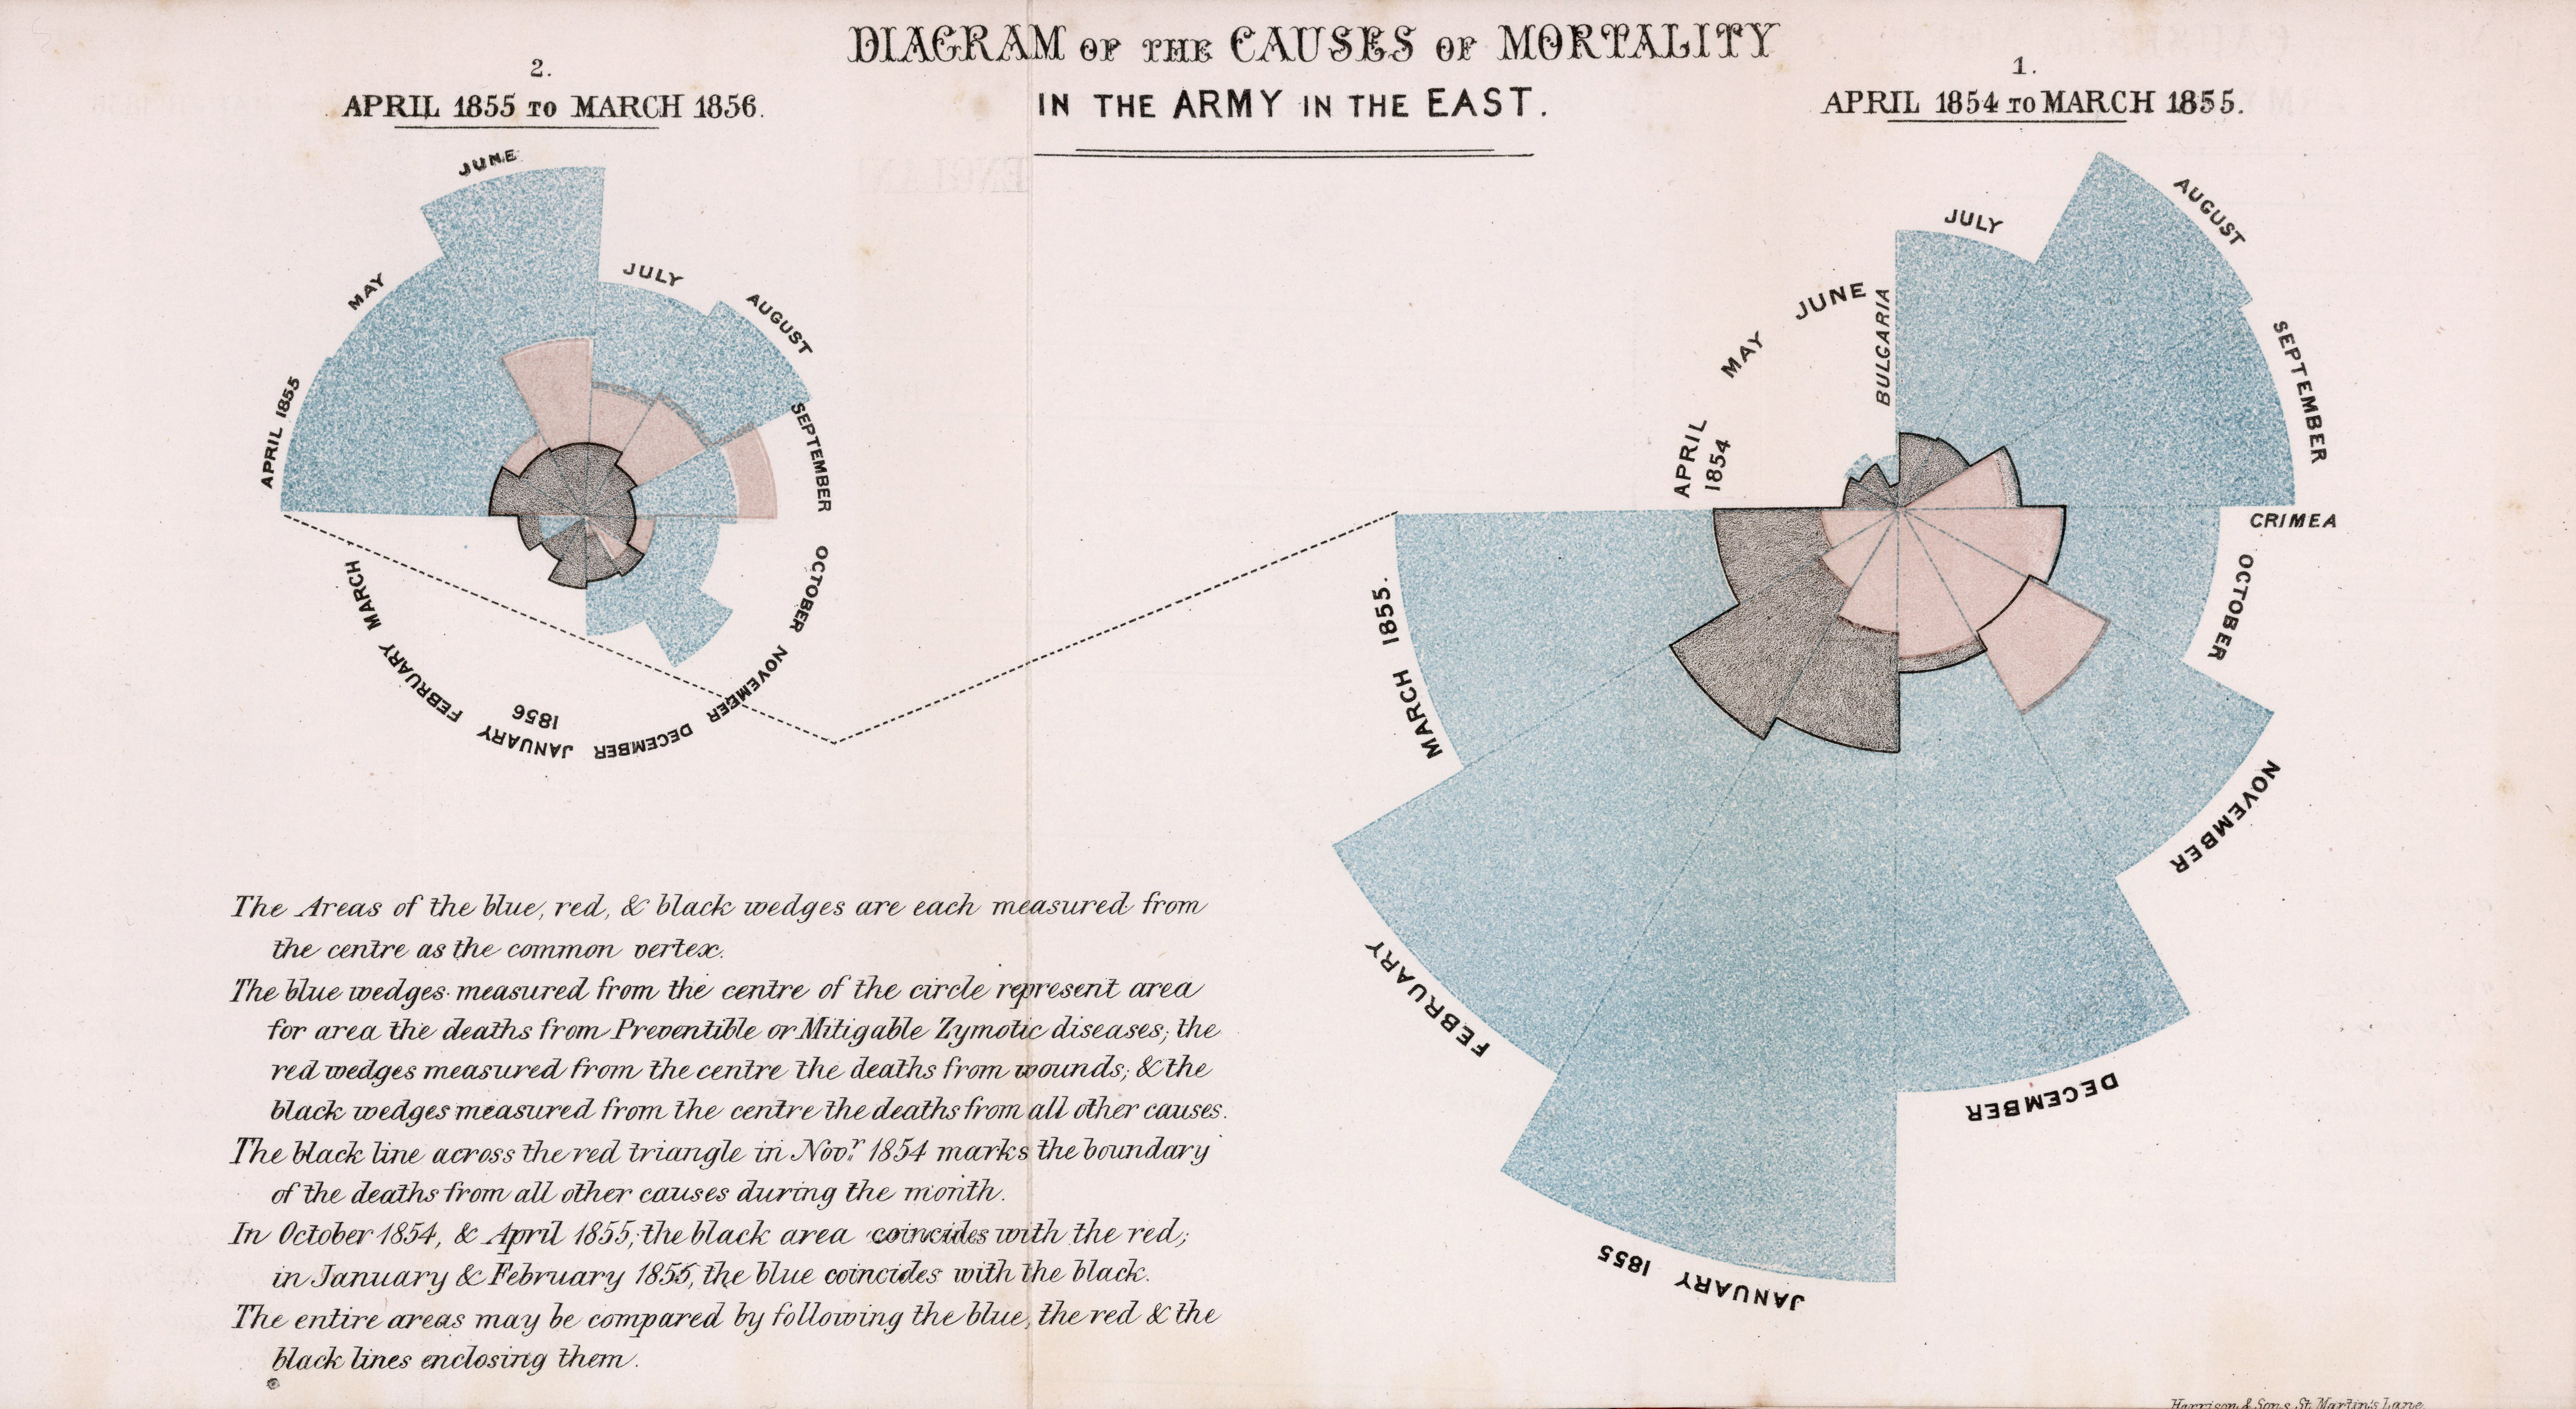
\includegraphics{images/Nightengale_diagram.jpg}

}

\caption{Florence Nightingale's (1858), ``Diagram of the causes of
mortality in the army in the East.'' A more effective pie chart where
the perceptual relative size issue is negated by the amount of
information conveyed and the potentially seasonal nature of the data.}

\end{figure}

\hypertarget{some-practicalities}{%
\section{Some Practicalities}\label{some-practicalities}}

The everyday graphs we make when conducting data analysis will usually
be more functional than pretty, but that doesn't have to stop us from
combining the two today. In the example below, we'll focus mainly on the
mechanics of constructing a visualization using \texttt{ggplot2} rather
than on how to use them analytically.

To get started, we'll load a new data set called \texttt{gapminder},
which contains data on countries. Conveniently, the \texttt{gapminder}
data is located in the \texttt{gapminder} package. As usual, we want to
be sure that we've installed the package before loading it for the first
time.

\begin{Shaded}
\begin{Highlighting}[]
\FunctionTok{library}\NormalTok{(gapminder)}
\FunctionTok{data}\NormalTok{(gapminder)}
\end{Highlighting}
\end{Shaded}

The \texttt{data()} function used above is an alternative to
\texttt{gapminder\ \textless{}-\ gapminder}. It loads the
\texttt{gapminder} data from the package into a \texttt{gapminder}
object in our environment. You can use either, but it's good to keep
learning new functions at this stage so that you can understand what
they do when you see them elsewhere.

As will become second nature to you to you soon, we can inspect this
data using \texttt{glimpse()}, \texttt{view()}, or by clicking on the
object in the environment pane.

\begin{Shaded}
\begin{Highlighting}[]
\FunctionTok{glimpse}\NormalTok{(gapminder)}
\end{Highlighting}
\end{Shaded}

\begin{verbatim}
Rows: 1,704
Columns: 6
$ country   <fct> "Afghanistan", "Afghanistan", "Afghanistan", "Afghanistan", ~
$ continent <fct> Asia, Asia, Asia, Asia, Asia, Asia, Asia, Asia, Asia, Asia, ~
$ year      <int> 1952, 1957, 1962, 1967, 1972, 1977, 1982, 1987, 1992, 1997, ~
$ lifeExp   <dbl> 28.801, 30.332, 31.997, 34.020, 36.088, 38.438, 39.854, 40.8~
$ pop       <int> 8425333, 9240934, 10267083, 11537966, 13079460, 14880372, 12~
$ gdpPercap <dbl> 779.4453, 820.8530, 853.1007, 836.1971, 739.9811, 786.1134, ~
\end{verbatim}

Our new tibble has 1,704 rows and 6 variables (\texttt{?gapminder}
provides some more information on the variables). There is something a
little bit different about this data compared to the GSS data. Whereas
in the GSS data each row corresponds to a separate observation (i.e., a
respondent), in the Gapminder data, each row corresponds to a year for a
particular country. We have, for instance, a row with data for
Afghanistan in 1952 and another row for Afghanistan in 1957 in the next.
The unit of observation here is called a ``country-year.'' Consider for
a moment how this might affect the answers you get when using
\texttt{mean()} or \texttt{median()}.

In the social sciences, we call this format, \textbf{long data}. The
differences in the way tabular data is stored has important implications
for the way we analyze it. We'll discuss this more in depth in the next
chapter. Luckily for us, the \texttt{gapminder} data is already in an
ideal format for \texttt{ggplot2}.

\hypertarget{brief-exercise}{%
\subsection*{Brief Exercise}\label{brief-exercise}}
\addcontentsline{toc}{subsection}{Brief Exercise}

As a brief exercise and to refresh your memory, let's use \texttt{dplyr}
to find the minimum and maximum years in the \texttt{gapminder} data.
Try it on your own first and then check your answer below.

\begin{tcolorbox}[enhanced jigsaw, colframe=quarto-callout-tip-color-frame, colback=white, title=\textcolor{quarto-callout-tip-color}{\faLightbulb}\hspace{0.5em}{Answer}, opacitybacktitle=0.6, coltitle=black, colbacktitle=quarto-callout-tip-color!10!white, arc=.35mm, leftrule=.75mm, bottomtitle=1mm, bottomrule=.15mm, breakable, opacityback=0, titlerule=0mm, rightrule=.15mm, left=2mm, toptitle=1mm, toprule=.15mm]

\begin{Shaded}
\begin{Highlighting}[]
\NormalTok{gapminder }\SpecialCharTok{\%\textgreater{}\%}
  \FunctionTok{summarize}\NormalTok{(}\AttributeTok{min\_year =} \FunctionTok{min}\NormalTok{(year),}
            \AttributeTok{max\_year =} \FunctionTok{max}\NormalTok{(year))}
\end{Highlighting}
\end{Shaded}

\begin{verbatim}
# A tibble: 1 x 2
  min_year max_year
     <int>    <int>
1     1952     2007
\end{verbatim}

\end{tcolorbox}

Now see whether you can find the minimum and maximum year for \emph{each
country} along with the number of times each country appears in the
data.

\begin{tcolorbox}[enhanced jigsaw, colframe=quarto-callout-tip-color-frame, colback=white, title=\textcolor{quarto-callout-tip-color}{\faLightbulb}\hspace{0.5em}{Answer}, opacitybacktitle=0.6, coltitle=black, colbacktitle=quarto-callout-tip-color!10!white, arc=.35mm, leftrule=.75mm, bottomtitle=1mm, bottomrule=.15mm, breakable, opacityback=0, titlerule=0mm, rightrule=.15mm, left=2mm, toptitle=1mm, toprule=.15mm]

\begin{Shaded}
\begin{Highlighting}[]
\NormalTok{gapminder }\SpecialCharTok{\%\textgreater{}\%}
  \FunctionTok{group\_by}\NormalTok{(country) }\SpecialCharTok{\%\textgreater{}\%}
    \FunctionTok{summarize}\NormalTok{(}\AttributeTok{min\_year =} \FunctionTok{min}\NormalTok{(year),}
              \AttributeTok{max\_year =} \FunctionTok{max}\NormalTok{(year),}
              \AttributeTok{n =} \FunctionTok{n}\NormalTok{())}
\end{Highlighting}
\end{Shaded}

\begin{verbatim}
# A tibble: 142 x 4
   country     min_year max_year     n
   <fct>          <int>    <int> <int>
 1 Afghanistan     1952     2007    12
 2 Albania         1952     2007    12
 3 Algeria         1952     2007    12
 4 Angola          1952     2007    12
 5 Argentina       1952     2007    12
 6 Australia       1952     2007    12
 7 Austria         1952     2007    12
 8 Bahrain         1952     2007    12
 9 Bangladesh      1952     2007    12
10 Belgium         1952     2007    12
# i 132 more rows
\end{verbatim}

\end{tcolorbox}

\hypertarget{how-ggplot2-works}{%
\section{\texorpdfstring{How \texttt{ggplot2}
Works}{How ggplot2 Works}}\label{how-ggplot2-works}}

Back to visualizations: much like a cake, \texttt{ggplot2} involves
adding layers. We start with a bare plot which has only our axes and
their labels and then we work our way up to the final product, layer by
layer.

\hypertarget{making-the-base-plot}{%
\subsection{Making the Base Plot}\label{making-the-base-plot}}

Just as with \texttt{dplyr}, we can use the pipe operator to work with
\texttt{ggplot2}. We first take the Gapminder data \emph{and then} add a
new function, \texttt{ggplot()}.

\begin{Shaded}
\begin{Highlighting}[]
\NormalTok{gapminder }\SpecialCharTok{\%\textgreater{}\%}
  \FunctionTok{ggplot}\NormalTok{()}
\end{Highlighting}
\end{Shaded}

\begin{figure}[H]

{\centering \includegraphics{visualizing-with-ggplot_files/figure-pdf/unnamed-chunk-14-1.pdf}

}

\end{figure}

Without any arguments supplied, the \texttt{ggplot()} function produces
a blank plot (shown above), a canvas we'll use to paint our
visualization. If you are following along in an R Script, you should be
able to see this plot in the lower right pane of your R Studio window
(under the `Plots' tab) after running it. We'd rather see a completed
canvas than a blank canvas, however, so we're going to supply an
argument called \texttt{mapping}. The \texttt{mapping} argument tells
\texttt{ggplot} how we are going to map the data to the plot.

\begin{verbatim}
gapminder %>%
  ggplot(mapping = )
\end{verbatim}

This mapping argument, in turn, requires us to specify an `aesthetic'
which will always be contained in an \texttt{aes()} function. So now we
have:

\begin{verbatim}
gapminder %>%
  ggplot(mapping = aes())
\end{verbatim}

If we were to run this, we would still get a blank plot. The
\texttt{ggplot()} function knows we're using the gapminder data (since
we used the pipe operator), but it doesn't yet know what we would like
to see on our x- or y-axes. For this, we need to define the aesthetic
characteristics of our plot.

Since our goal is to recreate the graph we saw in the beginning of this
chapter, which showed the relationship between GDP per capita
(\texttt{gdpPerCap}) and life expectancy (\texttt{lifeExp}), we'll
supply these variables to the \texttt{x} and \texttt{y} arguments inside
the \texttt{aes()} function.

\begin{Shaded}
\begin{Highlighting}[]
\NormalTok{gapminder }\SpecialCharTok{\%\textgreater{}\%}
  \FunctionTok{ggplot}\NormalTok{(}\AttributeTok{mapping =} \FunctionTok{aes}\NormalTok{(}\AttributeTok{x =}\NormalTok{ gdpPercap, }
                       \AttributeTok{y =}\NormalTok{ lifeExp))}
\end{Highlighting}
\end{Shaded}

\begin{figure}[H]

{\centering \includegraphics{visualizing-with-ggplot_files/figure-pdf/unnamed-chunk-15-1.pdf}

}

\end{figure}

Now we have a not-so-blank plot. We can see instead an x-axis, as
specified, showing \texttt{gdpPerCap}, and a y-axis, showing
\texttt{lifeExp}. But where are our data?

\hypertarget{specifying-the-type-of-plot}{%
\subsection{Specifying the Type of
Plot}\label{specifying-the-type-of-plot}}

In order to add data, we have to tell ggplot exactly what type of plot
we'd like to create. We could produce a scatterplot, for example, which
will cause the data to appear as points, or we could create a line
graph, which will connect points into lines. There are other options, of
course, but these seem like the most logical choices for this plot.

In \texttt{ggplot()}, the different types of plots are called
\emph{geoms} and we can add them as a layer to our base plot by using
the \texttt{+} operator followed by the \texttt{geom\_} function that
corresponds to the type of plot we want to see. If we wanted to see a
line plot, for instance, we would use \texttt{geom\_line()}. We want to
see a scatterplot, so we'll use the \texttt{geom\_point()} function.
Let's see how the scatterplot looks:

\begin{Shaded}
\begin{Highlighting}[]
\NormalTok{gapminder }\SpecialCharTok{\%\textgreater{}\%}
  \FunctionTok{ggplot}\NormalTok{(}\AttributeTok{mapping =} \FunctionTok{aes}\NormalTok{(}\AttributeTok{x =}\NormalTok{ gdpPercap, }
                       \AttributeTok{y =}\NormalTok{ lifeExp)) }\SpecialCharTok{+}
  \FunctionTok{geom\_point}\NormalTok{()}
\end{Highlighting}
\end{Shaded}

\begin{figure}[H]

{\centering \includegraphics{visualizing-with-ggplot_files/figure-pdf/unnamed-chunk-16-1.pdf}

}

\end{figure}

We now have a plot which shows us each country-year as a point. The
x-value is the GDP per capita of a country and the y-value is life
expectancy at birth, a measure of typical longevity. Notice, we didn't
need to supply an argument to \texttt{geom\_point()} nor did we have to
tell \texttt{ggplot()} anything other than the mapping of \texttt{x} and
\texttt{y} (and, of course, the initial source of data,
\texttt{gapminder}, via the pipe operator).

\texttt{ggplot} objects are unique in that we can add additional layers
by using the \texttt{+} operator to join them to the base plot and each
other. Just like with the pipe operator, however, we need to make sure
that the \texttt{+} appears at the end of each intermediate line and not
at the beginning of a line. Be on the lookout for these subtle syntax
errors:

\begin{verbatim}
# This will not produce a plot with points, 
# because the + operator is in the wrong spot.
gapminder %>%
  ggplot(mapping = aes(x = gdpPercap, 
                       y = lifeExp)) 
  + geom_point()
  
# This will produce a plot with points.
gapminder %>%
  ggplot(mapping = aes(x = gdpPercap, 
                       y = lifeExp)) +
  geom_point()
\end{verbatim}

\hypertarget{adding-a-smoother}{%
\subsection{Adding a Smoother}\label{adding-a-smoother}}

Can we add more layers to our plot? You bet. We can, for instance, add a
line of best fit on top of our points with a \texttt{geom\_smooth()}
function:

\begin{Shaded}
\begin{Highlighting}[]
\NormalTok{gapminder }\SpecialCharTok{\%\textgreater{}\%}
  \FunctionTok{ggplot}\NormalTok{(}\AttributeTok{mapping =} \FunctionTok{aes}\NormalTok{(}\AttributeTok{x =}\NormalTok{ gdpPercap, }
                       \AttributeTok{y =}\NormalTok{ lifeExp)) }\SpecialCharTok{+}
  \FunctionTok{geom\_point}\NormalTok{() }\SpecialCharTok{+} 
  \FunctionTok{geom\_smooth}\NormalTok{()}
\end{Highlighting}
\end{Shaded}

\begin{verbatim}
`geom_smooth()` using method = 'gam' and formula = 'y ~ s(x, bs = "cs")'
\end{verbatim}

\begin{figure}[H]

{\centering \includegraphics{visualizing-with-ggplot_files/figure-pdf/unnamed-chunk-17-1.pdf}

}

\end{figure}

The output warning here tells us that \texttt{geom\_smooth()} used a
default argument and formula to calculate the line of best
fit.\footnote{`gam' stands for general additive model and is one method
  of adding a line of best fit. `lm', or linear model, is another best
  fit method.}

\hypertarget{mapping-more-aesthetics}{%
\subsection{Mapping More Aesthetics}\label{mapping-more-aesthetics}}

What else can we do with this visualization? Well, we might want to see
if there are other elements that can be changed to reveal more patterns
in the data. What if we compared the country-level relationship between
\texttt{gdpPercap} and \texttt{lifeExp} by continent, for example? We
could create a plot for each continent, showing only the relevant
countries for each, or we could keep one plot and modify another element
like the color of the data points. In this way, each color would
represent the continent a country is located in and the points would be
visually differentiated.

To do this, we need to modify the aesthetics of our data mapping. We'll
add another argument to the \texttt{aes()} function inside of the
\texttt{ggplot()} mapping argument for \texttt{color}. And, of course,
since we want to color points by continent, we need to specify
\texttt{color\ =\ continent}. We'll skip the line of best fit this time.

\begin{Shaded}
\begin{Highlighting}[]
\NormalTok{gapminder }\SpecialCharTok{\%\textgreater{}\%}
  \FunctionTok{ggplot}\NormalTok{(}\AttributeTok{mapping =} \FunctionTok{aes}\NormalTok{(}\AttributeTok{x =}\NormalTok{ gdpPercap, }
                       \AttributeTok{y =}\NormalTok{ lifeExp,}
                       \AttributeTok{color =}\NormalTok{ continent)) }\SpecialCharTok{+}
  \FunctionTok{geom\_point}\NormalTok{()}
\end{Highlighting}
\end{Shaded}

\begin{figure}[H]

{\centering \includegraphics{visualizing-with-ggplot_files/figure-pdf/unnamed-chunk-18-1.pdf}

}

\end{figure}

Now we can see how the relationship between GDP and life expectancy
plays out among countries across different continents.

It might also be interesting to see how this relationship plays out by
population size. Since population size is a continuous quantitative
variable, discrete colors may not be a good choice. We could add a color
gradient scale (as you might see in a heat map, for example) or we could
modify some other element. What about changing the size of the points
according to population? Bigger countries could have larger points and
smaller countries could have smaller points with a continuum in between.
To do this, we need to add a size argument to the aesthetic mapping,
this time according to population (\texttt{pop}).

\begin{Shaded}
\begin{Highlighting}[]
\NormalTok{gapminder }\SpecialCharTok{\%\textgreater{}\%}
  \FunctionTok{ggplot}\NormalTok{(}\AttributeTok{mapping =} \FunctionTok{aes}\NormalTok{(}\AttributeTok{x =}\NormalTok{ gdpPercap, }
                       \AttributeTok{y =}\NormalTok{ lifeExp,}
                       \AttributeTok{color =}\NormalTok{ continent,}
                       \AttributeTok{size =}\NormalTok{ pop)) }\SpecialCharTok{+}
  \FunctionTok{geom\_point}\NormalTok{()}
\end{Highlighting}
\end{Shaded}

\begin{figure}[H]

{\centering \includegraphics{visualizing-with-ggplot_files/figure-pdf/unnamed-chunk-19-1.pdf}

}

\end{figure}

You can now see some trends for some specific countries, including a
certain rich and high population country in the Americas. Each time we
add an aesthetic,\texttt{ggplot()} makes the necessary change to the
plot and then adds a key to interpret each element. We now have scales
for population (the \texttt{size} value in our aesthetic mapping) and
continent (the \texttt{color} value in our mapping). Another optional
aesthetic argument you can use is \texttt{shape}, which changes the
points from dots to different symbols (like x's or o's). \texttt{line}
is another option which changes the type of line for
\texttt{geom\_line()}.

Because we have a lot of data points and they're overlapping, we're
going to skip shape and make it so that the points have some
transparency. We can do this by adding an \texttt{alpha} argument to the
\texttt{geom\_point()} component which controls transparency.
\texttt{alpha} takes a value between 0 and 1, where 0 is completely
translucent and 1 is not-transparent. We'll choose a halfway number,
\texttt{0.5}, but you can play around with the different levels to find
your preferred value.

\begin{Shaded}
\begin{Highlighting}[]
\NormalTok{gapminder }\SpecialCharTok{\%\textgreater{}\%}
  \FunctionTok{ggplot}\NormalTok{(}\AttributeTok{mapping =} \FunctionTok{aes}\NormalTok{(}\AttributeTok{x =}\NormalTok{ gdpPercap, }
                       \AttributeTok{y =}\NormalTok{ lifeExp,}
                       \AttributeTok{color =}\NormalTok{ continent,}
                       \AttributeTok{size =}\NormalTok{ pop)) }\SpecialCharTok{+}
  \FunctionTok{geom\_point}\NormalTok{(}\AttributeTok{alpha =} \FloatTok{0.5}\NormalTok{)}
\end{Highlighting}
\end{Shaded}

\begin{figure}[H]

{\centering \includegraphics{visualizing-with-ggplot_files/figure-pdf/unnamed-chunk-20-1.pdf}

}

\end{figure}

We are getting pretty close to the graph we started the chapter with. At
this point, we could add \texttt{geom\_smooth()} back to our plot. Take
a look at what happens when you do though.

\begin{Shaded}
\begin{Highlighting}[]
\NormalTok{gapminder }\SpecialCharTok{\%\textgreater{}\%}
  \FunctionTok{ggplot}\NormalTok{(}\AttributeTok{mapping =} \FunctionTok{aes}\NormalTok{(}\AttributeTok{x =}\NormalTok{ gdpPercap, }
                       \AttributeTok{y =}\NormalTok{ lifeExp,}
                       \AttributeTok{color =}\NormalTok{ continent,}
                       \AttributeTok{size =}\NormalTok{ pop)) }\SpecialCharTok{+}
  \FunctionTok{geom\_point}\NormalTok{(}\AttributeTok{alpha =} \FloatTok{0.5}\NormalTok{) }\SpecialCharTok{+}
  \FunctionTok{geom\_smooth}\NormalTok{()}
\end{Highlighting}
\end{Shaded}

\begin{verbatim}
`geom_smooth()` using method = 'loess' and formula = 'y ~ x'
\end{verbatim}

\begin{figure}[H]

{\centering \includegraphics{visualizing-with-ggplot_files/figure-pdf/unnamed-chunk-21-1.pdf}

}

\end{figure}

That's maybe not the result we thought it was going to be. Instead of
one smooth curve, as before, we now have a different colored curve for
each of the continents. We can also see in the key on the right-hand
side that population size is affecting the width of the lines as well.

One thing to know about \texttt{ggplot2} is that each item added to the
\texttt{ggplot()} object inherits \texttt{ggplot()}'s aesthetics. So
because we defined \texttt{color} by continent and \texttt{size} by
population in \texttt{ggplot()}'s mapping argument,
\texttt{geom\_point()} and \texttt{geom\_smooth()} are also also colored
by continent and sized by population.

If we want to instead ensure that the \texttt{color} and \texttt{size}
arguments only affect \texttt{geom\_point()}, we need to move those
aesthetics to \texttt{geom\_point()}'s own aesthetic mapping. See below:

\begin{Shaded}
\begin{Highlighting}[]
\NormalTok{gapminder }\SpecialCharTok{\%\textgreater{}\%}
  \FunctionTok{ggplot}\NormalTok{(}\AttributeTok{mapping =} \FunctionTok{aes}\NormalTok{(}\AttributeTok{x =}\NormalTok{ gdpPercap, }
                       \AttributeTok{y =}\NormalTok{ lifeExp)) }\SpecialCharTok{+}
  \FunctionTok{geom\_point}\NormalTok{(}\AttributeTok{mapping =} \FunctionTok{aes}\NormalTok{(}\AttributeTok{color =}\NormalTok{ continent,}
                       \AttributeTok{size =}\NormalTok{ pop),}
             \AttributeTok{alpha =} \FloatTok{0.5}\NormalTok{) }\SpecialCharTok{+}
  \FunctionTok{geom\_smooth}\NormalTok{()}
\end{Highlighting}
\end{Shaded}

\begin{verbatim}
`geom_smooth()` using method = 'gam' and formula = 'y ~ s(x, bs = "cs")'
\end{verbatim}

\begin{figure}[H]

{\centering \includegraphics{visualizing-with-ggplot_files/figure-pdf/unnamed-chunk-22-1.pdf}

}

\end{figure}

\texttt{geom\_point()}'s mapping accepts the same form of argument as
\texttt{ggplot()}. Let's remove \texttt{geom\_smooth()} again anyways,
since it doesn't seem particularly helpful and the plot looks better
without it. We can return the \texttt{color} and \texttt{size} arguments
to \texttt{ggplot()} or we can leave them as is. Just a few more changes
left before we get to a finished product.

\hypertarget{changing-scales}{%
\subsection{Changing Scales}\label{changing-scales}}

Let's change the x-axis scale to a logarithmic scale, since the data
appears to follow a logarithmic form. Scales can be changed by adding
functions from the \texttt{scale\_} family to our plot. Like
\texttt{geom\_}, there are a number of different options depending on
the need. In this case, we want a logarithmic scale for our x-axis in
base 10, so we'll use \texttt{scale\_x\_log10()}.

\begin{Shaded}
\begin{Highlighting}[]
\NormalTok{gapminder }\SpecialCharTok{\%\textgreater{}\%}
  \FunctionTok{ggplot}\NormalTok{(}\AttributeTok{mapping =} \FunctionTok{aes}\NormalTok{(}\AttributeTok{x =}\NormalTok{ gdpPercap, }
                       \AttributeTok{y =}\NormalTok{ lifeExp,}
                       \AttributeTok{size =}\NormalTok{ pop,}
                       \AttributeTok{color =}\NormalTok{ continent)) }\SpecialCharTok{+}
  \FunctionTok{geom\_point}\NormalTok{(}\AttributeTok{alpha =} \FloatTok{0.5}\NormalTok{) }\SpecialCharTok{+}
  \FunctionTok{scale\_x\_log10}\NormalTok{()}
\end{Highlighting}
\end{Shaded}

\begin{figure}[H]

{\centering \includegraphics{visualizing-with-ggplot_files/figure-pdf/unnamed-chunk-23-1.pdf}

}

\end{figure}

Now we can see the relationship between GDP per capita and life
expectancy more clearly. We don't always have to change the scale of our
x- and y-axes, but in this case, the distribution of our x-values calls
for it.\footnote{GDP per capita is not normally distributed hence the
  need for a log-transformation here. The decision on whether to
  transform an axis or not is a statistical matter, which we won't go
  into here.} If you don't add a \texttt{scale\_} function,
\texttt{ggplot2} will simply use the default. We don't need a scale
transformation for our y-axis here, so we'll skip adding a
\texttt{scale\_y\_} function and let \texttt{ggplot2} use the default.

Note that there is a conceptual difference between a scale (the numeric
distance between positions on some axis) and labels (how the values of
those different positions are recorded). Just because the numbers on the
axis are written in a strange or unhelpful format, in other words,
doesn't necessarily mean we that will need to change the scale. We may
just need to edit the labels. As you can see in our previous example,
even after the scale change, the x-axis labels are still not recorded in
the most legible format (scientific notation).

\hypertarget{changing-scale-labels}{%
\subsection{Changing Scale Labels}\label{changing-scale-labels}}

Changing the labels for axes and other scales can be a bit of a pain.
Fortunately, there is a very helpful package we can use called
\texttt{scales}.

You should already have a copy of \texttt{scales} installed and you can
load it via \texttt{library()}.\footnote{\texttt{scales} is contained in
  the \texttt{tidverse}, but it isn't automatically loaded when you use
  \texttt{library(tidyverse)}.} Another way to access it's functions is
to use the name of the package followed by \texttt{::} and the name of
the desired function. We used this same method in the previous chapter
for \texttt{knitr::kable()}.

For the scale on the x-axis, which corresponds to a variable in U.S.
dollars, we'll use the function
\texttt{scales::label\_currency()}.\footnote{The default currency for
  \texttt{label\_currency()} is U.S. dollars.} We'll add this helper
function to the \texttt{labels\ =} argument of our \texttt{scale\_}
function in the example below. Other useful \texttt{scales} functions
include \texttt{scales::comma} and \texttt{scales::percent} - neither of
which require parentheses at the end, unlike \texttt{label\_currency()}.

Since we also want to fix the label for the \texttt{size} function,
we'll also add a \texttt{scale\_} function for our size aesthetic (in a
separate object) and then set the \texttt{labels} argument to use
commas. See below for both steps put together:

\begin{Shaded}
\begin{Highlighting}[]
\NormalTok{gapminder }\SpecialCharTok{\%\textgreater{}\%}
  \FunctionTok{ggplot}\NormalTok{(}\AttributeTok{mapping =} \FunctionTok{aes}\NormalTok{(}\AttributeTok{x =}\NormalTok{ gdpPercap, }
                       \AttributeTok{y =}\NormalTok{ lifeExp,}
                       \AttributeTok{size =}\NormalTok{ pop,}
                       \AttributeTok{color =}\NormalTok{ continent)) }\SpecialCharTok{+}
  \FunctionTok{geom\_point}\NormalTok{(}\AttributeTok{alpha =} \FloatTok{0.5}\NormalTok{) }\SpecialCharTok{+} 
  \FunctionTok{scale\_x\_log10}\NormalTok{(}\AttributeTok{labels =}\NormalTok{ scales}\SpecialCharTok{::}\FunctionTok{label\_currency}\NormalTok{()) }\SpecialCharTok{+}
  \FunctionTok{scale\_size}\NormalTok{(}\AttributeTok{labels =}\NormalTok{ scales}\SpecialCharTok{::}\NormalTok{comma)}
\end{Highlighting}
\end{Shaded}

\begin{figure}[H]

{\centering \includegraphics{visualizing-with-ggplot_files/figure-pdf/unnamed-chunk-24-1.pdf}

}

\end{figure}

Our scale labels have been fixed and are much easier to read.

\hypertarget{adding-titles}{%
\subsection{Adding Titles}\label{adding-titles}}

To change the titles of different elements, we can add a \texttt{labs()}
function to the end of our object. The \texttt{labs()} function will set
titles for each part of the plot according to the values given to a set
of corresponding arguments.

In the code below, you can see that we've changed the title for the
\texttt{x} and \texttt{y} axes, the \texttt{size} key (``Population''),
the \texttt{color} key (``Continent''), the overall \texttt{title} of
the graph (``Economic Growth and Life Expectancy''), and then added a
\texttt{caption} at the bottom.

\begin{Shaded}
\begin{Highlighting}[]
\NormalTok{gapminder }\SpecialCharTok{\%\textgreater{}\%}
  \FunctionTok{ggplot}\NormalTok{(}\AttributeTok{mapping =} \FunctionTok{aes}\NormalTok{(}\AttributeTok{x =}\NormalTok{ gdpPercap, }
                       \AttributeTok{y =}\NormalTok{ lifeExp,}
                       \AttributeTok{size =}\NormalTok{ pop,}
                       \AttributeTok{color =}\NormalTok{ continent)) }\SpecialCharTok{+}
  \FunctionTok{geom\_point}\NormalTok{(}\AttributeTok{alpha =} \FloatTok{0.5}\NormalTok{) }\SpecialCharTok{+} 
  \FunctionTok{scale\_x\_log10}\NormalTok{(}\AttributeTok{labels =}\NormalTok{ scales}\SpecialCharTok{::}\FunctionTok{label\_currency}\NormalTok{()) }\SpecialCharTok{+}
  \FunctionTok{scale\_size}\NormalTok{(}\AttributeTok{labels =}\NormalTok{ scales}\SpecialCharTok{::}\NormalTok{comma) }\SpecialCharTok{+}
  \FunctionTok{labs}\NormalTok{(}\AttributeTok{x =} \StringTok{"GDP Per Capita (log scale)"}\NormalTok{,}
       \AttributeTok{y =} \StringTok{"Life Expectancy in Years"}\NormalTok{,}
       \AttributeTok{size =} \StringTok{"Population"}\NormalTok{,}
       \AttributeTok{color =} \StringTok{"Continent"}\NormalTok{,}
       \AttributeTok{title =} \StringTok{"Economic Growth and Life Expectancy"}\NormalTok{,}
       \AttributeTok{caption =} \StringTok{" Source: Gapminder }\SpecialCharTok{\textbackslash{}n}\StringTok{ Note: Observations are country{-}years."}\NormalTok{)}
\end{Highlighting}
\end{Shaded}

\begin{figure}[H]

{\centering \includegraphics{visualizing-with-ggplot_files/figure-pdf/unnamed-chunk-25-1.pdf}

}

\end{figure}

At this point, we have a good looking graph and could call it a day. As
you will discover though, there are endless opportunities for
customization with \texttt{ggplot2}. It's the reason why
\texttt{ggplot2} graphics can be made to look so good.

\hypertarget{adding-a-theme}{%
\subsection{Adding a Theme}\label{adding-a-theme}}

Themes are customizable sets of aesthetic characteristics that change
things like font types and sizes, the alignment of different elements,
and the presence of gridlines. You can adjust many of these things by
adding a \texttt{theme()} function to the end of your plot and playing
around with the different available arguments.

Alternatively, you can use a theme that someone else has created by
installing their package and using the related function. This is often
ideal, because you can then find a theme that matches your general
preferences and tweak minor elements as needed by overlaying another
\texttt{theme()} layer. Playing around with theme settings on your own
can be a time consuming affair and in general, isn't recommend for the
personal graphs you use for analytic purposes.

Among pre-packaged themes, \texttt{ggthemes}, for example, is a popular
package with themes that mimic the styles used in \emph{The Economist}
(\texttt{theme\_economist()}), for example, and the \emph{Wall Street
Journal} (\texttt{theme\_wsj()}). You can see some more of the styles
available in \texttt{ggthemes}
\href{https://yutannihilation.github.io/allYourFigureAreBelongToUs/ggthemes/}{here}.
The theme I used for the graph at the start of this chapter is called
\texttt{theme\_ipsum\_rc()} which comes from the \texttt{hrbrthemes}
package. Remember, if you use a theme from a package, you need to first
download the package and then load the library (or access the specific
function using \texttt{::}). Some custom themes, like ipsum, also
require you to install and register new fonts in \texttt{R}, which can
be a pain.

If you'd like to avoid the trouble of installing extra packages, you can
also use some of the default themes provided in \texttt{ggplot2}, many
of which are also quite nice. Adding \texttt{theme\_bw()} from
\texttt{ggplot2} to the plot from the previous example, for instance,
does this:

\begin{Shaded}
\begin{Highlighting}[]
\NormalTok{gapminder }\SpecialCharTok{\%\textgreater{}\%}
  \FunctionTok{ggplot}\NormalTok{(}\AttributeTok{mapping =} \FunctionTok{aes}\NormalTok{(}\AttributeTok{x =}\NormalTok{ gdpPercap, }
                       \AttributeTok{y =}\NormalTok{ lifeExp,}
                       \AttributeTok{size =}\NormalTok{ pop,}
                       \AttributeTok{color =}\NormalTok{ continent)) }\SpecialCharTok{+}
  \FunctionTok{geom\_point}\NormalTok{(}\AttributeTok{alpha =} \FloatTok{0.5}\NormalTok{) }\SpecialCharTok{+} 
  \FunctionTok{scale\_x\_log10}\NormalTok{(}\AttributeTok{labels =}\NormalTok{ scales}\SpecialCharTok{::}\FunctionTok{label\_currency}\NormalTok{()) }\SpecialCharTok{+}
  \FunctionTok{scale\_size}\NormalTok{(}\AttributeTok{labels =}\NormalTok{ scales}\SpecialCharTok{::}\NormalTok{comma) }\SpecialCharTok{+}
  \FunctionTok{labs}\NormalTok{(}\AttributeTok{x =} \StringTok{"GDP Per Capita (log scale)"}\NormalTok{,}
       \AttributeTok{y =} \StringTok{"Life Expectancy in Years"}\NormalTok{,}
       \AttributeTok{size =} \StringTok{"Population"}\NormalTok{,}
       \AttributeTok{color =} \StringTok{"Continent"}\NormalTok{,}
       \AttributeTok{title =} \StringTok{"Economic Growth and Life Expectancy"}\NormalTok{,}
       \AttributeTok{caption =} \StringTok{" Source: Gapminder }\SpecialCharTok{\textbackslash{}n}\StringTok{ Note: Observations are country{-}years."}\NormalTok{) }\SpecialCharTok{+}
  \FunctionTok{theme\_bw}\NormalTok{()}
\end{Highlighting}
\end{Shaded}

\begin{figure}[H]

{\centering \includegraphics{visualizing-with-ggplot_files/figure-pdf/unnamed-chunk-26-1.pdf}

}

\end{figure}

You can see that it has added a border to the plot and removed the gray
background from both the plot and the scales. Try using
\texttt{theme\_minimal()}, \texttt{theme\_classic()}, and
\texttt{theme\_void()} to see how they change the aesthetics instead.

\hypertarget{the-final-product}{%
\section{The Final Product}\label{the-final-product}}

To return to the final product, I'll use \texttt{theme\_ipsum\_rc()}
from \texttt{hrbrthemes}. I'll also replace the size\_scale argument
with a more complicated set of functions that makes it even easier to
read.

\begin{Shaded}
\begin{Highlighting}[]
\FunctionTok{library}\NormalTok{(hrbrthemes) }\CommentTok{\# A theme used for graphs}

\NormalTok{gapminder }\SpecialCharTok{\%\textgreater{}\%}
  \FunctionTok{ggplot}\NormalTok{(}\AttributeTok{mapping =} \FunctionTok{aes}\NormalTok{(}\AttributeTok{x =}\NormalTok{ gdpPercap, }
                       \AttributeTok{y =}\NormalTok{ lifeExp,}
                       \AttributeTok{size =}\NormalTok{ pop,}
                       \AttributeTok{color =}\NormalTok{ continent)) }\SpecialCharTok{+}
  \FunctionTok{geom\_point}\NormalTok{(}\AttributeTok{alpha =} \FloatTok{0.5}\NormalTok{) }\SpecialCharTok{+} 
  \FunctionTok{scale\_x\_log10}\NormalTok{(}\AttributeTok{labels =}\NormalTok{ scales}\SpecialCharTok{::}\FunctionTok{label\_currency}\NormalTok{()) }\SpecialCharTok{+}
  \FunctionTok{scale\_size}\NormalTok{(}\AttributeTok{labels =}\NormalTok{ scales}\SpecialCharTok{::}\FunctionTok{label\_number}\NormalTok{(}\AttributeTok{scale\_cut =}\NormalTok{ scales}\SpecialCharTok{::}\FunctionTok{cut\_short\_scale}\NormalTok{())) }\SpecialCharTok{+}
  \FunctionTok{labs}\NormalTok{(}\AttributeTok{x =} \StringTok{"GDP Per Capita (log scale)"}\NormalTok{,}
       \AttributeTok{y =} \StringTok{"Life Expectancy in Years"}\NormalTok{,}
       \AttributeTok{size =} \StringTok{"Population"}\NormalTok{,}
       \AttributeTok{color =} \StringTok{"Continent"}\NormalTok{,}
       \AttributeTok{title =} \StringTok{"Economic Growth and Life Expectancy"}\NormalTok{,}
       \AttributeTok{caption =} \StringTok{" Source: Gapminder }\SpecialCharTok{\textbackslash{}n}\StringTok{ Note: Observations are country{-}years."}\NormalTok{) }\SpecialCharTok{+}
  \FunctionTok{theme\_ipsum\_rc}\NormalTok{()}
\end{Highlighting}
\end{Shaded}

\begin{figure}[H]

{\centering \includegraphics{visualizing-with-ggplot_files/figure-pdf/unnamed-chunk-27-1.pdf}

}

\end{figure}

Whichever plot you choose to use as your final plot, you can save it by
clicking on the ``Plots'' tab in the lower right-hand corner of your R
Studio window followed by export. We'll discuss better ways of doing
this later on.

\hypertarget{other-plots}{%
\section{Other Plots}\label{other-plots}}

We've so far only covered one type of plot, a scatterplot. It won't
surprise you to learn that there are many other types of plots that we
can create using \texttt{ggplot2}. The good news is that the structure
and components of plots are generally consistent across types and that
once you start creating plots, you can always re-use the code.

A quick example of a line chart using the \texttt{gapminder} data is
shown below. Note, we've made a few changes. We first filtered the data
for a small subset of countries so that our graph won't be swamped with
too many countries. Then we used \texttt{geom\_line()} as our
\texttt{geom\_} instead of \texttt{geom\_point()}. Perhaps most
importantly, we've set \texttt{color} to represent each country in order
to ensure that our data is mapped to the appropriate unit of
observation.

\begin{Shaded}
\begin{Highlighting}[]
\NormalTok{my\_countries }\OtherTok{=} \FunctionTok{c}\NormalTok{(}\StringTok{\textquotesingle{}France\textquotesingle{}}\NormalTok{, }\StringTok{\textquotesingle{}United Kingdom\textquotesingle{}}\NormalTok{, }\StringTok{\textquotesingle{}Italy\textquotesingle{}}\NormalTok{)}

\NormalTok{gapminder }\SpecialCharTok{\%\textgreater{}\%}
  \FunctionTok{filter}\NormalTok{(country }\SpecialCharTok{\%in\%}\NormalTok{ my\_countries) }\SpecialCharTok{\%\textgreater{}\%}
  \FunctionTok{ggplot}\NormalTok{(}\FunctionTok{aes}\NormalTok{(}\AttributeTok{x =}\NormalTok{ year, }
             \AttributeTok{y =}\NormalTok{ pop, }
             \AttributeTok{color =}\NormalTok{ country)) }\SpecialCharTok{+}
  \FunctionTok{geom\_line}\NormalTok{()}
\end{Highlighting}
\end{Shaded}

\begin{figure}[H]

{\centering \includegraphics{visualizing-with-ggplot_files/figure-pdf/unnamed-chunk-28-1.pdf}

}

\end{figure}

Try setting \texttt{color\ =\ continent} in the example above and see
what happens. You end up with a bit of a mess. \texttt{ggplot2} doesn't
naturally understand the correct unit of observation, so specifying
continent as \texttt{color} leads it to believe that it needs connect
the data points according to the continent for each year and across
years. Since France, Italy, and the U.K. are in the same continent, it
draws a line connecting each of the three data points inside each year
and then connects them across years, leading to a jagged, meaningless
graph.

Here's a slightly more polished looking version of the initial line
graph with some aesthetic and label changes. We can easily change the
countries used and other features like the size of
\texttt{geom\_line()}. Perhaps confusingly, \texttt{geom\_line()} can
also take a \texttt{size} argument outside of the mapping argument. Note
also that you may wish to change the font family in the graphic below to
something like `Arial', since you may not have `Roboto Condensed'
installed on your computer.

\begin{Shaded}
\begin{Highlighting}[]
\NormalTok{my\_countries }\OtherTok{=} \FunctionTok{c}\NormalTok{(}\StringTok{\textquotesingle{}France\textquotesingle{}}\NormalTok{, }\StringTok{\textquotesingle{}United Kingdom\textquotesingle{}}\NormalTok{, }\StringTok{\textquotesingle{}Italy\textquotesingle{}}\NormalTok{)}

\NormalTok{gapminder }\SpecialCharTok{\%\textgreater{}\%}
  \FunctionTok{filter}\NormalTok{(country }\SpecialCharTok{\%in\%}\NormalTok{ my\_countries) }\SpecialCharTok{\%\textgreater{}\%}
  \FunctionTok{ggplot}\NormalTok{(}\FunctionTok{aes}\NormalTok{(}\AttributeTok{x =}\NormalTok{ year, }
             \AttributeTok{y =}\NormalTok{ pop, }
             \AttributeTok{color =}\NormalTok{ country)) }\SpecialCharTok{+}
  \FunctionTok{geom\_line}\NormalTok{(}\AttributeTok{size =} \DecValTok{2}\NormalTok{) }\SpecialCharTok{+}  
  \FunctionTok{scale\_y\_continuous}\NormalTok{(}\AttributeTok{labels =}\NormalTok{ scales}\SpecialCharTok{::}\FunctionTok{label\_number}\NormalTok{(}\AttributeTok{scale\_cut =}\NormalTok{ scales}\SpecialCharTok{::}\FunctionTok{cut\_short\_scale}\NormalTok{())) }\SpecialCharTok{+} 
  \FunctionTok{labs}\NormalTok{(}\AttributeTok{x=}\StringTok{"Year"}\NormalTok{,}
       \AttributeTok{y =} \StringTok{"Population"}\NormalTok{,}
       \AttributeTok{color =} \StringTok{"Country"}\NormalTok{,}
       \AttributeTok{title =} \StringTok{"Population Growth in Europe"}\NormalTok{,}
       \AttributeTok{caption =} \StringTok{"Source: Gapminder"}\NormalTok{) }\SpecialCharTok{+} 
  \FunctionTok{theme\_bw}\NormalTok{() }\SpecialCharTok{+} 
  \FunctionTok{theme}\NormalTok{(}\AttributeTok{text =} \FunctionTok{element\_text}\NormalTok{(}\AttributeTok{size =} \DecValTok{14}\NormalTok{, }\AttributeTok{family =} \StringTok{"Roboto Condensed"}\NormalTok{),}
                     \AttributeTok{plot.title =} \FunctionTok{element\_text}\NormalTok{(}\AttributeTok{size =} \DecValTok{20}\NormalTok{, }\AttributeTok{face =} \StringTok{"bold"}\NormalTok{),}
                     \AttributeTok{axis.title.x =} \FunctionTok{element\_text}\NormalTok{(}\AttributeTok{hjust=}\DecValTok{1}\NormalTok{), }
                     \AttributeTok{axis.title.y =} \FunctionTok{element\_text}\NormalTok{(}\AttributeTok{hjust=}\DecValTok{1}\NormalTok{))}
\end{Highlighting}
\end{Shaded}

\begin{figure}[H]

{\centering \includegraphics{visualizing-with-ggplot_files/figure-pdf/unnamed-chunk-29-1.pdf}

}

\end{figure}

Last, but not least, we have a bar chart. Here again we've filtered for
some countries. We've then filtered for a specific year, removed color
(which works slightly differently for bar charts), and have added the
\texttt{geom\_col()} geom to specify that it is a bar chart we are
making.

\begin{Shaded}
\begin{Highlighting}[]
\NormalTok{my\_countries }\OtherTok{=} \FunctionTok{c}\NormalTok{(}\StringTok{\textquotesingle{}France\textquotesingle{}}\NormalTok{, }\StringTok{\textquotesingle{}United Kingdom\textquotesingle{}}\NormalTok{, }\StringTok{\textquotesingle{}Italy\textquotesingle{}}\NormalTok{, }\StringTok{"Germany"}\NormalTok{, }\StringTok{"Spain"}\NormalTok{)}

\NormalTok{gapminder }\SpecialCharTok{\%\textgreater{}\%}
  \FunctionTok{filter}\NormalTok{(country }\SpecialCharTok{\%in\%}\NormalTok{ my\_countries) }\SpecialCharTok{\%\textgreater{}\%}
  \FunctionTok{filter}\NormalTok{(year }\SpecialCharTok{==} \DecValTok{2007}\NormalTok{) }\SpecialCharTok{\%\textgreater{}\%}
  \FunctionTok{ggplot}\NormalTok{(}\AttributeTok{mapping =} \FunctionTok{aes}\NormalTok{(}\AttributeTok{x =}\NormalTok{ country, }
                       \AttributeTok{y =}\NormalTok{ pop)) }\SpecialCharTok{+}  
  \FunctionTok{geom\_col}\NormalTok{()}
\end{Highlighting}
\end{Shaded}

\begin{figure}[H]

{\centering \includegraphics{visualizing-with-ggplot_files/figure-pdf/unnamed-chunk-30-1.pdf}

}

\end{figure}

We will work through other examples of visualizations, such as the map
below, and the quirks of how they work in future chapters.

\includegraphics{visualizing-with-ggplot_files/figure-pdf/unnamed-chunk-31-1.pdf}

\hypertarget{summary-1}{%
\section{Summary}\label{summary-1}}

In this chapter, we've reviewed some of the measures we might use to
describe data, discussed some general principles for producing good data
visualizations, and learned how to create and modify some basic plots in
\texttt{ggplot2}.

You will likely need to read this chapter and reference the code more
than once. \texttt{ggplot2}'s structure is not very intuitive to new
users. The more you use it, however, and get a feel for how the
different plot elements map to the various objects and arguments, the
more control you will have over the visualizations you produce.

So keep practicing and save your work, adding comments so that you can
remember what you were doing. Go back to some of the examples used here
and play around with the different arguments. Try to change the plot
types. Use different scales. See if you can make something interesting.
As you inevitably get errors, try to make a mental note of what works
and what doesn't. Eventually, you'll have generated a stockpile of code
that you can re-use and adjust to create the right visualizations
whenever you need them.

\hypertarget{exercises}{%
\section{Exercises}\label{exercises}}

Here are a few exercises to complete either in-class or on your own for
homework.

\begin{enumerate}
\def\labelenumi{\arabic{enumi}.}
\item
  Use the Gapminder data to produce a line graph showing growth in GDP
  per capita for the United Kingdom, France and Italy.
\item
  Do the same for life expectancy using three other countries of your
  choice.
\item
  Produce a scatterplot which shows the relationship between GDP per
  capita and life expectancy for all countries in 2007. Produce another
  which shows the relationship for 1952 and compare the two.
\item
  Produce a bar chart for life expectancy among countries in Oceania in
  2007.
\end{enumerate}

\bookmarksetup{startatroot}

\hypertarget{workflows-and-wrangling}{%
\chapter{Workflows and Wrangling}\label{workflows-and-wrangling}}

At this point in the course, we have primarily been working with data
from packages, which is generally convenient and straight forward. We
install the package with the data we want, we load the package from the
library, and then we access the data and begin summarizing it. The bad
news is that the data we might want to use for a particular project
oftentimes isn't contained in a package. The even worse news is that we
usually need to clean and transform the data in order to get it into a
format that works for analysis.

This chapter covers some of the processes and functions in \texttt{R}
made for dealing with these unfortunate eventualities. We'll start with
the general problem of working with files in \texttt{R}, then learn how
to get data in, and then we'll learn more about how to make data
analyzable.

This chapter will not, of course, provide you with the answers to all of
the data wrangling problems you will eventually encounter. It will
barely scratch the surface. But, once you manage to get data in, data
wrangling becomes a matter of learning new functions and practicing the
tidy data skills you've already started to learn.

\hypertarget{whats-happening-under-the-hood}{%
\section{What's Happening Under the
Hood?}\label{whats-happening-under-the-hood}}

Up until now, we've been writing our code in plain-text files saved with
a \texttt{.R} file extension (or what we've been calling R script files)
and we haven't needed to load data from other files or to save anything.

That last part isn't entirely true though. We have actually been loading
data from files saved on our computers. It just so happens that the
packages we installed earlier and the \texttt{library()} function have
gone to great lengths to simplify and conceal the back-end interactions
that led to data showing up in our RStudio environment. All of this data
is saved somewhere on our computers, we just might not know where it is.

As with any type of computer program, \texttt{R} itself operates from
somewhere on your hard drive. It uses data, functions, and other
compiled code which have been saved across a number of files (and file
types) in different locations to run the program and allow us to
interact with it. This is the case for everything software-related, from
the apps on your smartphone to the operating system on your laptop. It's
all running from code saved somewhere in the device's memory.

For this chapter, we don't have to go deep into the code that composes
\texttt{R} or \texttt{RStudio}. All we need to know, instead, is how to
get \texttt{R} to interact with files saved in different locations on
our computer as well as how to organize them in a way that makes them
easy to work with.

\hypertarget{file-structures-file-paths-and-the-working-directory}{%
\section{File Structures, File Paths, and the Working
Directory}\label{file-structures-file-paths-and-the-working-directory}}

Your computer's operating system (Windows, MacOS, or Linux) organizes
the files on your computer into folders. You might have created some
folders on your own, renamed them, or stored files like photos,
documents, and other items across them. Pictures might go in a
``Pictures'' folder, for example, and documents in a ``Documents''
folder. You might have a ``Sciences Po'' folder and then a sub-folder
for ``SPSSUR.''\footnote{You may also have all of your files saved on
  your ``Desktop'' folder, in which case, you should consider applying
  the Marie Kondo principles of tidying up to your digital spaces. A
  minor caveat, though, which is that sparking joy may not be a good
  criteria for computer system files.}

The way files are organized across folders and sub-folders on a
computer's hard drive is usually referred to as your computer's
\textbf{file structure}. Within a file structure, each file has a
\textbf{file path}, which is an address that identifies where the file
is located. In Windows, they usually look something like this:

\begin{verbatim}
"C:\Users\wcs26\Documents\Sciences Po\SPSSUR\my_file.R"
\end{verbatim}

In MacOS, they might look more like this:

\begin{verbatim}
"/Users/wcs26/Documents/Sciences Po/SPSSUR/my_file.R"
\end{verbatim}

As an important aside, when you write file paths in \texttt{R}, you will
generally want to write them in the MacOS format you see above (i.e.,
using forwards slashes, \texttt{/}) even if you are using a PC. This is
because the backwards slash, \texttt{\textbackslash{}}, is a special
character in \texttt{R}.

Within the operating systems themselves, file paths are slightly easier
to find in Windows than in MacOS since you can get most of the way there
by clicking in the address bar at the top of a Windows Explorer window
(see below for an example).\footnote{Note that if you copy and paste a
  path from a Windows Explorer into \texttt{R}, you'll have to change
  the direction of the \texttt{\textbackslash{}} to \texttt{/} or deal
  with the \texttt{\textbackslash{}} issue in a different way (there are
  other ways, but hopefully you won't need to copy and paste paths
  anyways).} This gives the folder path, which when followed by another
slash, the file name, and the file extension, gives the file path. In
MacOS, finding a file path requires a little more effort (see
\href{https://support.apple.com/en-mt/guide/mac-help/mchlp1774/mac\#:~:text=On\%20your\%20Mac\%2C\%20click\%20the,bottom\%20of\%20the\%20Finder\%20window.}{here}
for some guidance).\footnote{If you are using a Linux-based OS, you
  probably won't need an explanation of file structures and file paths,
  given the greater transparency of file paths and structures you
  regularly encounter.}

\includegraphics[width=6.22917in,height=\textheight]{images/Windows-file-path.PNG}

When working with multiple files in \texttt{R}, as you will in more
involved analysis projects, you will need to pay some attention to the
file structure and file paths. When you load data from a file, for
instance, \texttt{R} will need to know exactly where the file is
located. If you are saving a graph, similarly, \texttt{R} will need to
know where you want to save it.

\texttt{R} makes an educated guess as to where in your file structure
you are working from based on how you open your \texttt{R} session. This
is called the \textbf{working directory} and you can identify where
\texttt{R} has located it using the command below:

\begin{Shaded}
\begin{Highlighting}[]
\FunctionTok{getwd}\NormalTok{()}
\end{Highlighting}
\end{Shaded}

Sometimes the working directory doesn't quite match where you think it
should be and you might need to change it manually as a result. We will
endeavor to avoid this when we can, but if you must, you can always
manually set it using \texttt{setwd()}.

\hypertarget{the-problem-with-file-paths}{%
\section{The Problem with File
Paths}\label{the-problem-with-file-paths}}

Functions that load data generally require you to provide a file path
that leads to the data file. The problem with file structures and file
paths, however, is that everyone's is different. So, if we have a file
saved in a specific location on our computer and then some code that
reads it, how do we make sure that other people can use our code when
their file structure is going to be different?

To make this more concrete, let's say that I send you an R Script along
with a data file called \texttt{important\_data.csv}, so that you can
replicate some analysis and visualizations I did. In that R Script, I
might have a line that looks like this:

\begin{verbatim}
read_csv("C:/Users/wcs26/Documents/Sciences Po/SPSSUR/important_data.csv")
\end{verbatim}

This command will try to read in a data file,
\texttt{important\_data.csv}, located within \texttt{C:/}, the
\texttt{Users/} folder, the \texttt{wcs26/} folder, and so on and so
forth. As soon as you run it, \texttt{R} will attempt to read the file
located at the end of this path by working its way through the file
structure. As soon as it hits a folder it can't find on your computer,
however, it will stop and produce an error that looks something like
this:

\begin{verbatim}
Error: 'C:/Users/wcs26/Documents/Sciences Po/SPSSUR/important_data.csv' does not exist.
\end{verbatim}

This type of file path construction, in which every folder and
sub-folder on the way to the destination is provided, is called an
\textbf{absolute} file path. If any part of the address is incorrect,
\texttt{R} won't be able to find the file, the file won't be read, and
the code fails to run. So, what's the alternative?

Well, one solution is to use what are called \textbf{relative} file
paths. A relative file path might look something like this:

\begin{verbatim}
read_csv("important_data.csv")
\end{verbatim}

In this case, because we haven't provided the full address, \texttt{R}
fills in the rest by guessing and, naturally, it guesses that the
missing part of the address is the working directory (i.e.,
\texttt{C:/Users/wcs26/Documents/Sciences\ Po/SPSSUR/}). If \texttt{R}
guessed correctly and the file is located in your working directory,
then this works perfectly fine and the data will be read correctly. If
the file isn't located in the working directory, however, it will fail.

The trouble is that sometimes you might start your \texttt{R} session in
one place and then open files from another place. Since \texttt{R} can
only keep track of one working directory at a time per session, it (or
rather you) will get confused quickly and your relative file paths will
also fail.

\hypertarget{r-projects-and-here}{%
\section{\texorpdfstring{R Projects and
\texttt{here}}{R Projects and here}}\label{r-projects-and-here}}

Fortunately, there is a better way. To avoid these working directory
problems and hard-coding absolute file paths in scripts, we're going to
use two solutions that will help keep them straight.

\hypertarget{r-projects}{%
\subsection{R Projects}\label{r-projects}}

The first is R Projects, a tool to organize your files in R Studio. When
you create an R Project file (\texttt{.Rproj}), R Studio creates a new
folder on your computer which is made to store all of the associated
files you may have for a project (e.g., your data, your code, and any
outputs). Every time you open that R Project file, R Studio opens a new
working session with a working directory correctly set to the location
of your project file. All of your files will be right where you need
them.

Let's create one for today's classwork. In R Studio, use the navigation
bar at the top of your screen to go to \texttt{File} \textgreater{}
\texttt{New\ Project} \textgreater{} \texttt{New\ Directory}
\textgreater{} \texttt{New\ Project}. Then, in the provided prompt, type
in a project name that matches our course naming standards (e.g.,
``Stubenbord\_Wesley\_Session 5 Classwork''). Create this project as a
sub-directory of your SPSSUR course folder (wherever this may be and
whatever it may be called on your computer). Once this has been created,
this is where your projects files will live, a permanent home just for
them. You can verify that the new project folder has been created by
navigating to it in your computer's file browser (e.g., Windows Explorer
in Windows).

\includegraphics[width=4.26042in,height=\textheight]{images/Creating-R-Project.PNG}

After you create a new project, you'll find yourself in a clean R Studio
session with only a console window open. The folder in your computer
system will contain just the new \texttt{.Rproj} file and a sub-folder
with some saved settings. This \texttt{.Rproj} file is how you will
access your project from now on. Instead of opening a .R script to
access your code, you'll always want to open your \texttt{.Rproj} file
first and then the .R script second. Don't put anything in this new
folder other than files directly associated with the project you are
working on. In this case, that means that this folder is only intended
to store files associated with today's classwork.

\includegraphics[width=5.03125in,height=\textheight]{images/R-Project-Folder.PNG}

Back in R Studio, in the lower-right hand pane with the ``Files'' tab,
you'll see all of the files currently associated with the project. At
the moment, there shouldn't be anything apart from the \texttt{.Rproj}
file itself).

In this same ``Files'' tab, you can add a new R Script file to this
project by clicking on the ``New Blank File'' button \textgreater{} ``R
Script''. Go ahead and create one and then save it with an appropriate
file name.

\includegraphics{images/R-Project-RStudio-Window.PNG}

Running \texttt{getwd()} from your new script file or directly in the
console will show you that your working directory does indeed match your
R Project location. Huzzah.

\includegraphics{images/R-project-getwd.PNG}

\hypertarget{here}{%
\subsection{\texorpdfstring{\texttt{here}}{here}}\label{here}}

The second tool is a package called \texttt{here}. \texttt{here}
contains a useful function, called \texttt{here()}, which will help
ensure that your code is always oriented to the correct working
directory: the location of the associated R Project file. There are some
occasions where, despite our best efforts, R Projects won't save us from
erroneous working directories. \texttt{here} helps cover those cases.

We'll come back to the application of this function in a moment, but for
now, install \texttt{here}, load it, and test the \texttt{here()}
function.

\begin{Shaded}
\begin{Highlighting}[]
\CommentTok{\#install.packages(\textquotesingle{}here\textquotesingle{})}
\FunctionTok{library}\NormalTok{(here)}
\end{Highlighting}
\end{Shaded}

\begin{verbatim}
here() starts at C:/Users/wcs26/OneDrive/Documents/College/7_Ph.D/Sciences Po/Statistical Programming for the Social Sciences/SPSSUR Textbook
\end{verbatim}

\begin{Shaded}
\begin{Highlighting}[]
\FunctionTok{here}\NormalTok{()}
\end{Highlighting}
\end{Shaded}

\begin{verbatim}
[1] "C:/Users/wcs26/OneDrive/Documents/College/7_Ph.D/Sciences Po/Statistical Programming for the Social Sciences/SPSSUR Textbook"
\end{verbatim}

You should see, again, the correct working directory for your R Project.

\hypertarget{organizing-your-project}{%
\subsection{Organizing Your Project}\label{organizing-your-project}}

RProjects and \texttt{here}, while both extremely useful, also won't
spare you entirely from the task of organizing your project files. A
clean and organized work space will make your life significantly easier
in the long-run. To facilitate this, I always recommend creating a
sub-folder within your project directory to store data sets (called
\texttt{data} for example), an additional sub-folder to store figure or
graphs (called \texttt{figures}, for example), and another to store
documentation (called \texttt{docs} for example). These sub-folder names
are commonly used among programmers and also help to ensure consistency
across projects with many collaborators. You can create these folders
directly in R Studio using the ``New Folder'' button near the top of the
`Files' tab in the lower-right hand pane.

\includegraphics{images/R-Project-sub-folders.PNG}

When finished, you will have your code in the main project folder along
with the \texttt{.RProj} file and several affiliated sub-folders for
storing things later.

\hypertarget{getting-data-into-r}{%
\section{\texorpdfstring{Getting Data into
\texttt{R}}{Getting Data into R}}\label{getting-data-into-r}}

Let us get back to the primordial problem now, which is getting data
into \texttt{R}. In the social sciences, the data we use can come from a
variety of different sources: we might take our data from long-running
surveys, for instance, such as the \href{https://gss.norc.org/}{General
Social Survey}, the
\href{https://www.europeansocialsurvey.org/}{European Social Survey}, or
the \href{https://www.worldvaluessurvey.org/}{World Values Survey}. We
can also use administrative data produced by government agencies, like
the Federal Bureau of Investigation's
\href{https://www.fbi.gov/how-we-can-help-you/more-fbi-services-and-information/ucr}{Uniform
Crime Reports} or data from New York City's
\href{https://opendata.cityofnewyork.us/}{Open Data} initiative.

Alternatively, we can use data from other sources, which may not have
been produced with research or administrative purposes in mind. For
example, we can scrape data from social media to see how political
sentiment changes in times of crises or we can use data from online
dating apps to see how social norms around courtship have changed.

In any case, the most common format you are likely to find data stored
in is a CSV file, which stands for comma separated values. CSVs are
particularly appealing for data storage because they are lightweight and
they simple. They don't contain any extra formatting - all they consist
of is plain-text data in rows (separated by new lines) and columns
(separated by commas). A CSV file could consist of the following, for
example:

\begin{verbatim}
"id","name","age","country"
1011232,"Bill Gates",75,"United States"
1022234,"Warren Buffet",82,"United States"
\end{verbatim}

When you open a CSV file in software like Microsoft Excel, it is usually
automatically parsed into different columns, based on the position of
the commas, and into different rows, based on the line
breaks.\footnote{\textbf{Parsing} refers to how software reads the
  values.} Excel will automatically recognize, for example, that name is
a column containing two values, ``Bill Gates'' in one row and ``Warren
Buffett'' in another. CSVs don't always use commas to separate their
values - sometimes (especially in Europe), they use semi-colons. The
character (e.g., \texttt{,} or \texttt{;}) that separates values in a
data file is called a \textbf{delimiter}.

\includegraphics[width=6.32292in,height=\textheight]{images/excel-parsing.PNG}

\hypertarget{loading-files-from-csvs}{%
\section{Loading files from CSVs}\label{loading-files-from-csvs}}

Thankfully, loading CSV files is not very difficult in \texttt{R}.
\texttt{R} has a base function for loading CSVs, \texttt{read.csv()},
but there is a better version called \texttt{read\_csv()} which comes
from the \texttt{readr} package. \texttt{readr} is also located in the
\texttt{tidyverse}, but must also be loaded separately, just like the
\texttt{scales} package in the previous chapter.\footnote{As before,
  rather than load the entire \texttt{readr} package via
  \texttt{library()}, you can also use the \texttt{::} syntax, as in
  \texttt{readr::read\_csv()}.}

On the course Moodle site, you'll find a CSV titled
\texttt{billionaires\_2020-2023.csv}, which contains some limited data
on the world's billionaires from my own research. Go ahead and download
this file and then save it in the \texttt{data} sub-folder you created
in your \texttt{Session\ 5\ Classwork} project folder. Open the
\texttt{Session\ 5\ Classwork} project and a script file inside of it,
if you haven't already. We'll load a few libraries first and then the
data set.

\begin{Shaded}
\begin{Highlighting}[]
\FunctionTok{library}\NormalTok{(tidyverse)}
\end{Highlighting}
\end{Shaded}

\begin{verbatim}
-- Attaching core tidyverse packages ------------------------ tidyverse 2.0.0 --
v dplyr     1.1.4     v readr     2.1.5
v forcats   1.0.0     v stringr   1.5.1
v ggplot2   3.5.0     v tibble    3.2.1
v lubridate 1.9.3     v tidyr     1.3.1
v purrr     1.0.2     
-- Conflicts ------------------------------------------ tidyverse_conflicts() --
x dplyr::filter() masks stats::filter()
x dplyr::lag()    masks stats::lag()
i Use the conflicted package (<http://conflicted.r-lib.org/>) to force all conflicts to become errors
\end{verbatim}

\begin{Shaded}
\begin{Highlighting}[]
\FunctionTok{library}\NormalTok{(readr)}
\FunctionTok{library}\NormalTok{(here)}
\end{Highlighting}
\end{Shaded}

As with any function that reads data, \texttt{read\_csv()} requires a
file path to locate the data nad read it into our \texttt{R} session.
Because the data set is located in a sub-folder and because we want to
use a relative path (rather than an absolute path), we'll use
\texttt{here()}.

Remember, \texttt{here()} provides the file path to your R Project
folder. Any additional folder or file names used as arguments inside of
the \texttt{here()} function (separated by a comma) will be added to the
project folder path. If your R Project folder is located at
\texttt{C:\textbackslash{}Users\textbackslash{}Documents\textbackslash{}My\ Projects},
for example, \texttt{here("data")} will output
\texttt{C:\textbackslash{}Users\textbackslash{}Documents\textbackslash{}My\ Projects\textbackslash{}data}.
You must enclose the name of your sub-folders in quotation marks.

Entering the following should return the file path of the data set if
you have saved it within your \texttt{data} subfolder:

\begin{Shaded}
\begin{Highlighting}[]
\FunctionTok{here}\NormalTok{(}\StringTok{"data"}\NormalTok{,}\StringTok{"billionaires\_2020{-}2023.csv"}\NormalTok{)}
\end{Highlighting}
\end{Shaded}

\begin{verbatim}
[1] "C:/Users/wcs26/OneDrive/Documents/College/7_Ph.D/Sciences Po/Statistical Programming for the Social Sciences/SPSSUR Textbook/data/billionaires_2020-2023.csv"
\end{verbatim}

To read the actual data into \texttt{R}, now all we need to do is put
this \texttt{here} function inside of \texttt{read\_csv()} in the
\texttt{file\ =} argument.

\begin{Shaded}
\begin{Highlighting}[]
\FunctionTok{read\_csv}\NormalTok{(}\AttributeTok{file =} \FunctionTok{here}\NormalTok{(}\StringTok{"data"}\NormalTok{,}\StringTok{"billionaires\_2020{-}2023.csv"}\NormalTok{))}
\end{Highlighting}
\end{Shaded}

\begin{verbatim}
Rows: 2640 Columns: 13
-- Column specification --------------------------------------------------------
Delimiter: ","
chr (8): name, gender, country, countrycode, region, marital, residence_coun...
dbl (5): id, 2020, 2021, 2022, 2023

i Use `spec()` to retrieve the full column specification for this data.
i Specify the column types or set `show_col_types = FALSE` to quiet this message.
\end{verbatim}

\begin{verbatim}
# A tibble: 2,640 x 13
      id name        gender country countrycode region marital residence_country
   <dbl> <chr>       <chr>  <chr>   <chr>       <chr>  <chr>   <chr>            
 1     1 A. Jayson ~ male   United~ USA         North~ Married United States    
 2     9 Abdulla Al~ male   United~ ARE         Middl~ Married United Arab Emir~
 3    10 Abdulla bi~ male   United~ ARE         Middl~ <NA>    United Arab Emir~
 4    12 Abdulsamad~ male   Nigeria NGA         Sub-S~ Married Nigeria          
 5    13 Abhay Firo~ male   India   IND         South~ Married India            
 6    14 Abhay Soi   male   India   IND         South~ <NA>    <NA>             
 7    16 Abigail Be~ female United~ USA         North~ <NA>    <NA>             
 8    17 Abigail Jo~ female United~ USA         North~ Married United States    
 9    18 Abilio dos~ male   Brazil  BRA         Latin~ Married Brazil           
10    20 Acharya Ba~ male   India   IND         South~ Single  India            
# i 2,630 more rows
# i 5 more variables: selfmade <chr>, `2020` <dbl>, `2021` <dbl>, `2022` <dbl>,
#   `2023` <dbl>
\end{verbatim}

As you can see from the output above, \texttt{read\_csv()} worked! If
our data had used a semi-colon as a delimiter instead of a comma, we
would have just used \texttt{read\_csv2()} instead.

We can see from the resulting output that this data set has 2,640 rows
and 13 columns. Let's save this into a new object in our environment.

\begin{Shaded}
\begin{Highlighting}[]
\NormalTok{billionaires }\OtherTok{\textless{}{-}} \FunctionTok{read\_csv}\NormalTok{(}\AttributeTok{file =} \FunctionTok{here}\NormalTok{(}\StringTok{"data"}\NormalTok{,}\StringTok{"billionaires\_2020{-}2023.csv"}\NormalTok{))}
\end{Highlighting}
\end{Shaded}

\begin{verbatim}
Rows: 2640 Columns: 13
-- Column specification --------------------------------------------------------
Delimiter: ","
chr (8): name, gender, country, countrycode, region, marital, residence_coun...
dbl (5): id, 2020, 2021, 2022, 2023

i Use `spec()` to retrieve the full column specification for this data.
i Specify the column types or set `show_col_types = FALSE` to quiet this message.
\end{verbatim}

You'll notice that \texttt{read\_csv()} says a lot each time you run it.
Don't confuse the red text you see here with errors, however. It's just
trying to be helpful by giving you some more information about the data
we're reading in. We can see from this output, for example, that there
are 8 character columns and 5 \texttt{dbl} columns. \texttt{dbl} stands
for \texttt{double} and is a type of numeric value. We can, of course,
use \texttt{glimpse()} to see the variables again along with some of the
first few values.

\begin{Shaded}
\begin{Highlighting}[]
\FunctionTok{glimpse}\NormalTok{(billionaires)}
\end{Highlighting}
\end{Shaded}

\begin{verbatim}
Rows: 2,640
Columns: 13
$ id                <dbl> 1, 9, 10, 12, 13, 14, 16, 17, 18, 20, 25, 26, 27, 29~
$ name              <chr> "A. Jayson Adair", "Abdulla Al Futtaim", "Abdulla bi~
$ gender            <chr> "male", "male", "male", "male", "male", "male", "fem~
$ country           <chr> "United States", "United Arab Emirates", "United Ara~
$ countrycode       <chr> "USA", "ARE", "ARE", "NGA", "IND", "IND", "USA", "US~
$ region            <chr> "North America", "Middle East & North Africa", "Midd~
$ marital           <chr> "Married", "Married", NA, "Married", "Married", NA, ~
$ residence_country <chr> "United States", "United Arab Emirates", "United Ara~
$ selfmade          <chr> "self-made", "self-made", "inherited", "self-made", ~
$ `2020`            <dbl> NA, 2.437, 4.293, 3.365, 1.740, NA, NA, 12.531, 2.66~
$ `2021`            <dbl> 1.110, 2.441, 3.107, 5.437, 2.663, NA, NA, 23.189, 2~
$ `2022`            <dbl> 1.140, 2.591, 2.695, 7.151, 2.902, NA, NA, 21.971, 2~
$ `2023`            <dbl> 1.3, 2.4, 3.0, 8.2, 2.7, 1.2, 1.1, 21.6, 2.4, 3.4, 2~
\end{verbatim}

There are other ways you can take a peek at your data. We can take a
random slice of the data using \texttt{slice\_sample()} from
\texttt{dplyr}, for example. We can also use \texttt{slice\_head()} to
see the first few rows, \texttt{slice\_tail()} to see the last few rows,
or \texttt{slice\_min()} and \texttt{slice\_max()} to see the rows with
the largest or smallest values for some variable. Give them each a try
and look at their documentation to see some helpful optional arguments
you can use as well, like \texttt{n\ =}.

\begin{Shaded}
\begin{Highlighting}[]
\NormalTok{billionaires }\SpecialCharTok{\%\textgreater{}\%}
  \FunctionTok{slice\_sample}\NormalTok{(}\AttributeTok{n =} \DecValTok{5}\NormalTok{)}
\end{Highlighting}
\end{Shaded}

\begin{verbatim}
# A tibble: 5 x 13
     id name         gender country countrycode region marital residence_country
  <dbl> <chr>        <chr>  <chr>   <chr>       <chr>  <chr>   <chr>            
1  3347 Philip Ansc~ male   United~ USA         North~ Married United States    
2  3602 Robert Kraft male   United~ USA         North~ Widowed United States    
3  4334 Vivek Chaan~ male   Austra~ AUS         East ~ Married India            
4  3782 Savitri Jin~ female India   IND         South~ Widowed India            
5  2193 K. Dinesh    male   India   IND         South~ Married India            
# i 5 more variables: selfmade <chr>, `2020` <dbl>, `2021` <dbl>, `2022` <dbl>,
#   `2023` <dbl>
\end{verbatim}

No matter how we choose to do it, though, our purpose at this point of
reading data in should always be to get a sense for any potential issues
lurking beneath the surface of our data file.

You may have noticed from \texttt{glimpse} that there is something a
little bit weird about this data. Four columns at the end have numbers
as titles. What are these columns? Since this data doesn't come from a
package and there's no documentation, I will tell you: they're the
estimated net worth of each of the listed individuals in billions of
2023-inflation adjusted dollars for each of the named years (i.e., 2020,
2021, 2022, 2023). The values are in billions of US dollars.\footnote{The
  net worth estimates here are derived from the Forbes' annual
  \emph{World's Billionaires} list and inflation-adjusted using an
  implict GDP price deflator from the U.S. Federal Reserve.}

Now that we know what the data is, we can start to make sense of it. We
can use \texttt{slice\_max()} , for instance, to see who was the richest
person in 2023. In this case, note that when we reference a variable
which begins with a number, we have to use the
\texttt{\textasciigrave{}} character to enclose the variable name. This
is because \texttt{R} does not allow object names to start with a
number.

\begin{Shaded}
\begin{Highlighting}[]
\NormalTok{billionaires }\SpecialCharTok{\%\textgreater{}\%}
  \FunctionTok{slice\_max}\NormalTok{(}\StringTok{\textasciigrave{}}\AttributeTok{2023}\StringTok{\textasciigrave{}}\NormalTok{, }\AttributeTok{n =} \DecValTok{1}\NormalTok{)}
\end{Highlighting}
\end{Shaded}

\begin{verbatim}
# A tibble: 1 x 13
     id name         gender country countrycode region marital residence_country
  <dbl> <chr>        <chr>  <chr>   <chr>       <chr>  <chr>   <chr>            
1   425 Bernard Arn~ male   France  FRA         Europ~ Married France           
# i 5 more variables: selfmade <chr>, `2020` <dbl>, `2021` <dbl>, `2022` <dbl>,
#   `2023` <dbl>
\end{verbatim}

Now we can see that Bernard Arnault was the richest person in 2023 with
an estimated net worth of \$211 billion. What if we want to see what the
cumulative net worth of all French billionaires was for the years
covered in this data? Maybe we could use \texttt{dplyr} to summarize:

\begin{Shaded}
\begin{Highlighting}[]
\NormalTok{billionaires }\SpecialCharTok{\%\textgreater{}\%}
  \FunctionTok{group\_by}\NormalTok{(country) }\SpecialCharTok{\%\textgreater{}\%}
  \FunctionTok{filter}\NormalTok{(country }\SpecialCharTok{==} \StringTok{"France"}\NormalTok{) }\SpecialCharTok{\%\textgreater{}\%}
  \FunctionTok{summarize}\NormalTok{(}\AttributeTok{total\_nw =} \FunctionTok{sum}\NormalTok{())}
\end{Highlighting}
\end{Shaded}

\begin{verbatim}
# A tibble: 1 x 2
  country total_nw
  <chr>      <int>
1 France         0
\end{verbatim}

Here we run into a problem. We can't \texttt{group\_by(country,\ year)},
because there is no variable called \texttt{year}. There's also no
\texttt{net\_worth} variable that we can put into our
\texttt{summarize()} function. So, we're stuck with bad options. We
could try something like this, for example:

\begin{Shaded}
\begin{Highlighting}[]
\NormalTok{billionaires }\SpecialCharTok{\%\textgreater{}\%}
  \FunctionTok{group\_by}\NormalTok{(country) }\SpecialCharTok{\%\textgreater{}\%}
  \FunctionTok{filter}\NormalTok{(country }\SpecialCharTok{==} \StringTok{"France"}\NormalTok{) }\SpecialCharTok{\%\textgreater{}\%}
  \FunctionTok{summarize}\NormalTok{(}\AttributeTok{nw\_2023 =} \FunctionTok{sum}\NormalTok{(}\StringTok{\textasciigrave{}}\AttributeTok{2023}\StringTok{\textasciigrave{}}\NormalTok{),}
            \AttributeTok{nw\_2022 =} \FunctionTok{sum}\NormalTok{(}\StringTok{\textasciigrave{}}\AttributeTok{2022}\StringTok{\textasciigrave{}}\NormalTok{),}
            \AttributeTok{nw\_2021 =} \FunctionTok{sum}\NormalTok{(}\StringTok{\textasciigrave{}}\AttributeTok{2021}\StringTok{\textasciigrave{}}\NormalTok{),}
            \AttributeTok{nw\_2020 =} \FunctionTok{sum}\NormalTok{(}\StringTok{\textasciigrave{}}\AttributeTok{2020}\StringTok{\textasciigrave{}}\NormalTok{))}
\end{Highlighting}
\end{Shaded}

\begin{verbatim}
# A tibble: 1 x 5
  country nw_2023 nw_2022 nw_2021 nw_2020
  <chr>     <dbl>   <dbl>   <dbl>   <dbl>
1 France     585.      NA      NA      NA
\end{verbatim}

That got us the total net worth of French billionaires in 2023, at
least, but it didn't calculate a result for the other years. The reason
why we're having a hard time here is that our data is not in the right
format for \texttt{tidyverse} functions.

\hypertarget{tidy-data}{%
\section{Tidy Data}\label{tidy-data}}

In the previous chapter, we learned that the \texttt{gapminder} data was
in just the right format for \texttt{ggplot}. We called this
\textbf{long} format data, which is usally how we describe this format
in the social sciences. In a long format, rows are repeated observations
for some unit of analysis (like a country) across some dimension (like
time). In the case of the \texttt{gapminder} data, each of these
observations (country-years) had a value for a set of variables of
interest (e.g., life expectancy and GDP per capita) as shown below.

\begin{longtable}[]{@{}lrrr@{}}
\toprule\noalign{}
country & year & lifeExp & gdpPercap \\
\midrule\noalign{}
\endhead
\bottomrule\noalign{}
\endlastfoot
France & 1952 & 67.41 & 7029.809 \\
France & 1957 & 68.93 & 8662.835 \\
France & 1962 & 70.51 & 10560.486 \\
France & 1967 & 71.55 & 12999.918 \\
France & 1972 & 72.38 & 16107.192 \\
\end{longtable}

In the \texttt{billionaires} data, we instead have one row per unit of
analysis (billionaires) and multiple columns for a single variable of
interest (net worth).

\begin{longtable}[]{@{}rlrrrr@{}}
\toprule\noalign{}
id & name & 2020 & 2021 & 2022 & 2023 \\
\midrule\noalign{}
\endhead
\bottomrule\noalign{}
\endlastfoot
1 & A. Jayson Adair & NA & 1.110 & 1.140 & 1.3 \\
9 & Abdulla Al Futtaim & 2.437 & 2.441 & 2.591 & 2.4 \\
10 & Abdulla bin Ahmad Al Ghurair & 4.293 & 3.107 & 2.695 & 3.0 \\
\end{longtable}

The column titles (e.g., 2020, 2021), to be clear, are not actually
different variables, they are simply values of a single variable (e.g.,
year). When data is split in this way, we say it is in a \textbf{wide}
format. Wide data does have it's uses. It is very convenient, for
instance, for storing a large amount of data in a small amount of space
- a particular concern when you are printing data sets. Long data, on
the other hand, is much better for data analysis.

The \texttt{tidyverse} functions require data to be in what Hadley
Wickham and collaborators call a \textbf{tidy} format. In tidy data,
each variable is in a column, each observation is in a row, and each
cell contains a single value (Wickham et al.~2019). It is, in other
words, in a consistent \emph{long}-format. If we want to be able to use
all of the great features of \texttt{dplyr} and \texttt{ggplot}, we need
to transform our data into a tidy format.

\hypertarget{pivoting-from-wide-to-long}{%
\section{Pivoting from Wide to Long}\label{pivoting-from-wide-to-long}}

Fortunately, \texttt{dplyr} has some handy functions for this. Since we
have data in a wide format and wish to change it to a long format, we'll
need to use a function called \texttt{pivot\_longer()}. There are three
arguments we need to provide to \texttt{pivot\_longer()}.

First, in the \texttt{cols\ =} argument, we need to provide the columns
we are trying to combine into a single variable. In our case, our net
worth values are distributed across the
\texttt{\textasciigrave{}2020\textasciigrave{}},
\texttt{\textasciigrave{}2021\textasciigrave{}},
\texttt{\textasciigrave{}2022\textasciigrave{}}, and
\texttt{\textasciigrave{}2023\textasciigrave{}} columns, so we'll put
those in a vector and use them for this argument. Next, in the
\texttt{names\_to\ =} argument, we need to identify where we want to put
the names for each of those values (in other words, the titles for each
of our former columns). Since each of those column names corresponds to
a year, we'll tell it to put them in a \texttt{"year"} column. Last, we
need to specify a name for the variable holding all of the values that
were stored across those columns. Since the values were net worth, we'll
call this new variable \texttt{net\_worth}. We might also want to drop
the rows which contain NA values for net worth and so we'll add an
optional fourth argument, \texttt{values\_drop\_na\ =}.

\begin{Shaded}
\begin{Highlighting}[]
\NormalTok{billionaires }\SpecialCharTok{\%\textgreater{}\%}
  \FunctionTok{pivot\_longer}\NormalTok{(}\AttributeTok{cols =} \FunctionTok{c}\NormalTok{(}\StringTok{\textasciigrave{}}\AttributeTok{2020}\StringTok{\textasciigrave{}}\NormalTok{, }\StringTok{\textasciigrave{}}\AttributeTok{2021}\StringTok{\textasciigrave{}}\NormalTok{, }\StringTok{\textasciigrave{}}\AttributeTok{2022}\StringTok{\textasciigrave{}}\NormalTok{, }\StringTok{\textasciigrave{}}\AttributeTok{2023}\StringTok{\textasciigrave{}}\NormalTok{),}
               \AttributeTok{names\_to =} \StringTok{"year"}\NormalTok{,}
               \AttributeTok{values\_to =} \StringTok{"net\_worth"}\NormalTok{,}
               \AttributeTok{values\_drop\_na =} \ConstantTok{TRUE}\NormalTok{)}
\end{Highlighting}
\end{Shaded}

\begin{verbatim}
# A tibble: 9,142 x 11
      id name        gender country countrycode region marital residence_country
   <dbl> <chr>       <chr>  <chr>   <chr>       <chr>  <chr>   <chr>            
 1     1 A. Jayson ~ male   United~ USA         North~ Married United States    
 2     1 A. Jayson ~ male   United~ USA         North~ Married United States    
 3     1 A. Jayson ~ male   United~ USA         North~ Married United States    
 4     9 Abdulla Al~ male   United~ ARE         Middl~ Married United Arab Emir~
 5     9 Abdulla Al~ male   United~ ARE         Middl~ Married United Arab Emir~
 6     9 Abdulla Al~ male   United~ ARE         Middl~ Married United Arab Emir~
 7     9 Abdulla Al~ male   United~ ARE         Middl~ Married United Arab Emir~
 8    10 Abdulla bi~ male   United~ ARE         Middl~ <NA>    United Arab Emir~
 9    10 Abdulla bi~ male   United~ ARE         Middl~ <NA>    United Arab Emir~
10    10 Abdulla bi~ male   United~ ARE         Middl~ <NA>    United Arab Emir~
# i 9,132 more rows
# i 3 more variables: selfmade <chr>, year <chr>, net_worth <dbl>
\end{verbatim}

If we take a look at the data now, we can see that we've increased our
number of rows substantially (to 9,142) and each net worth value is now
in a separate row according to the corresponding year and individual. It
looks tidy. Now we can do much of the same type of data analysis and
visualization we have been doing over the past couple of chapters.

\begin{Shaded}
\begin{Highlighting}[]
\CommentTok{\# A quick and dirty plot.}
\NormalTok{tidy\_bil }\OtherTok{\textless{}{-}}\NormalTok{ billionaires }\SpecialCharTok{\%\textgreater{}\%}
  \FunctionTok{pivot\_longer}\NormalTok{(}\AttributeTok{cols =} \FunctionTok{c}\NormalTok{(}\StringTok{\textasciigrave{}}\AttributeTok{2020}\StringTok{\textasciigrave{}}\NormalTok{, }\StringTok{\textasciigrave{}}\AttributeTok{2021}\StringTok{\textasciigrave{}}\NormalTok{, }\StringTok{\textasciigrave{}}\AttributeTok{2022}\StringTok{\textasciigrave{}}\NormalTok{, }\StringTok{\textasciigrave{}}\AttributeTok{2023}\StringTok{\textasciigrave{}}\NormalTok{),}
               \AttributeTok{names\_to =} \StringTok{"year"}\NormalTok{,}
               \AttributeTok{values\_to =} \StringTok{"net\_worth"}\NormalTok{,}
               \AttributeTok{values\_drop\_na =} \ConstantTok{TRUE}\NormalTok{)}

\NormalTok{tidy\_bil }\SpecialCharTok{\%\textgreater{}\%}
  \FunctionTok{group\_by}\NormalTok{(country, year) }\SpecialCharTok{\%\textgreater{}\%}
  \FunctionTok{filter}\NormalTok{(country }\SpecialCharTok{==} \StringTok{"France"}\NormalTok{) }\SpecialCharTok{\%\textgreater{}\%}
  \FunctionTok{summarize}\NormalTok{(}\AttributeTok{agg\_nw =} \FunctionTok{sum}\NormalTok{(net\_worth)) }\SpecialCharTok{\%\textgreater{}\%}
  \FunctionTok{ggplot}\NormalTok{(}\AttributeTok{mapping =} \FunctionTok{aes}\NormalTok{(}\AttributeTok{x =}\NormalTok{ year, }\AttributeTok{y =}\NormalTok{ agg\_nw, }\AttributeTok{group =}\NormalTok{ country)) }\SpecialCharTok{+} 
  \FunctionTok{geom\_line}\NormalTok{(}\AttributeTok{linewidth =} \DecValTok{2}\NormalTok{) }\SpecialCharTok{+}
  \FunctionTok{labs}\NormalTok{(}\AttributeTok{title =} \StringTok{"The Wealth of France\textquotesingle{}s Billionaires"}\NormalTok{,}
       \AttributeTok{x =} \StringTok{"Year"}\NormalTok{,}
       \AttributeTok{y =} \StringTok{"Net Worth (USD in Billions)"}\NormalTok{) }\SpecialCharTok{+} 
  \FunctionTok{theme\_minimal}\NormalTok{()}
\end{Highlighting}
\end{Shaded}

\begin{verbatim}
`summarise()` has grouped output by 'country'. You can override using the
`.groups` argument.
\end{verbatim}

\begin{figure}[H]

{\centering \includegraphics{workflows-and-wrangling_files/figure-pdf/unnamed-chunk-15-1.pdf}

}

\end{figure}

\hypertarget{merging-data}{%
\section{Merging Data}\label{merging-data}}

Let's say that we want to do some further analysis involving additional
data not contained in the data set we are currently using. Can we add it
to our existing data set? The answer is yes.

On the course Moodle site, you'll find another data set called
\texttt{age.xlsx}. This is an Excel file. Fortunately, the
\texttt{readxl} package (also contained in the \texttt{tidverse} and
requiring separate loading) has just the function. Download the file
from the Moodle page, add it to your project's data folder, and then use
the command below:

\begin{Shaded}
\begin{Highlighting}[]
\FunctionTok{library}\NormalTok{(readxl)}

\NormalTok{bil\_age }\OtherTok{\textless{}{-}} \FunctionTok{read\_xlsx}\NormalTok{(}\AttributeTok{path =} \FunctionTok{here}\NormalTok{(}\StringTok{"data"}\NormalTok{, }\StringTok{"age.xlsx"}\NormalTok{), }\AttributeTok{sheet =} \StringTok{"Sheet1"}\NormalTok{)}

\FunctionTok{glimpse}\NormalTok{(bil\_age)}
\end{Highlighting}
\end{Shaded}

\begin{verbatim}
Rows: 2,724
Columns: 3
$ id   <dbl> 1, 9, 12, 13, 14, 16, 17, 18, 20, 25, 26, 27, 29, 32, 33, 34, 36,~
$ year <dbl> 2023, 2023, 2023, 2023, 2023, 2023, 2023, 2023, 2023, 2023, 2023,~
$ age  <dbl> 53, 83, 62, 78, 49, 42, 61, 86, 50, 40, 44, 81, 39, 54, 52, 39, 6~
\end{verbatim}

As we can see from the output, there isn't too much in here, just an ID,
a year, and an age. If we want to use this data in our next analysis, we
now need to merge it with our previously tidied data. We might just want
to check the \texttt{year} column to see how many years this age data
covers.

\begin{Shaded}
\begin{Highlighting}[]
\NormalTok{bil\_age }\SpecialCharTok{\%\textgreater{}\%}
  \FunctionTok{distinct}\NormalTok{(year)}
\end{Highlighting}
\end{Shaded}

\begin{verbatim}
# A tibble: 2 x 1
   year
  <dbl>
1  2023
2    NA
\end{verbatim}

\begin{Shaded}
\begin{Highlighting}[]
\CommentTok{\#An alternative way:}
\CommentTok{\#unique(bil\_age$year)}
\end{Highlighting}
\end{Shaded}

There's only one year, unfortunately, and quite a few missing values.
Before we go ahead and merge, we should also check to make sure that
there is only one age value for each ID. Merging data with multiple
values for each unit of analysis will cause rather large problems. Keep
a careful eye on your data as you do these types of things. The code
below will count the number of rows:

\begin{Shaded}
\begin{Highlighting}[]
\NormalTok{bil\_age }\SpecialCharTok{\%\textgreater{}\%}
  \FunctionTok{count}\NormalTok{(id) }\SpecialCharTok{\%\textgreater{}\%}
  \FunctionTok{filter}\NormalTok{(n }\SpecialCharTok{\textgreater{}} \DecValTok{1}\NormalTok{)}
\end{Highlighting}
\end{Shaded}

\begin{verbatim}
# A tibble: 59 x 2
      id     n
   <dbl> <int>
 1     1     4
 2     9     2
 3    12     5
 4    13     5
 5    14     2
 6    15     2
 7    16     2
 8    17     5
 9    18     5
10    19     2
# i 49 more rows
\end{verbatim}

It looks like there are a few duplicates in here. We can investigate
further, but let's see if dropping the NAs fixes our problem. They won't
be useful in our analysis later anyways.

\begin{Shaded}
\begin{Highlighting}[]
\NormalTok{bil\_age }\SpecialCharTok{\%\textgreater{}\%}
  \FunctionTok{drop\_na}\NormalTok{(age) }\SpecialCharTok{\%\textgreater{}\%}
  \FunctionTok{count}\NormalTok{(id) }\SpecialCharTok{\%\textgreater{}\%}
  \FunctionTok{filter}\NormalTok{(n }\SpecialCharTok{\textgreater{}} \DecValTok{1}\NormalTok{)}
\end{Highlighting}
\end{Shaded}

\begin{verbatim}
# A tibble: 0 x 2
# i 2 variables: id <dbl>, n <int>
\end{verbatim}

Good, no results, which means that dropping the NAs solved our problem
with duplicates. Let's save the tibble without the missing values and
carry on with our merge.

\begin{Shaded}
\begin{Highlighting}[]
\NormalTok{bil\_age }\SpecialCharTok{\%\textgreater{}\%}
  \FunctionTok{drop\_na}\NormalTok{(age) }\OtherTok{{-}\textgreater{}}\NormalTok{ bil\_age}
\end{Highlighting}
\end{Shaded}

Note that we've used our assignment operator in a somewhat unorthodox
way here. Instead of using it at the beginning of the piped function,
we've added it to the end. This works and is also acceptable.

Now, let's merge. Here, we'll use a function from \texttt{dplyr} called
\texttt{left\_join()}. There are other types of \texttt{\_join()}
functions depending on the use case. In our case, we have an existing
data set and we simply want to add data from another tibble to it. We
don't care much about what happens to the rows in the \texttt{bil\_age}
data set that don't match up. We'll use \texttt{left\_join()} as a
result. Other types of joins include \texttt{right\_join()},
\texttt{inner\_join()}, \texttt{left\_join()} and \texttt{full\_join()}.
Take a look at the supporting documentation to learn more about them.

\begin{Shaded}
\begin{Highlighting}[]
\FunctionTok{left\_join}\NormalTok{(}\AttributeTok{x =}\NormalTok{ tidy\_bil, }
          \AttributeTok{y =}\NormalTok{ bil\_age, }
          \FunctionTok{join\_by}\NormalTok{(id, year))}
\end{Highlighting}
\end{Shaded}

This didn't quite work and, if we look at our error, we can see why. The
\texttt{year} column in our \texttt{tidy\_bil} data is a character and
the the \texttt{year} column in our age data is a double. We'll have to
convert the column in \texttt{tidy\_bil} to continue. We should probably
convert \texttt{year} to a date format, but we're going to cheat here
and just convert it to a numeric variable for convenience. Hopefully
this won't come back to bite us later.

\begin{Shaded}
\begin{Highlighting}[]
\NormalTok{tidy\_bil }\SpecialCharTok{\%\textgreater{}\%}
  \FunctionTok{mutate}\NormalTok{(}\AttributeTok{year =} \FunctionTok{as.numeric}\NormalTok{(year)) }\OtherTok{{-}\textgreater{}}\NormalTok{ tidy\_bil}
\end{Highlighting}
\end{Shaded}

Let's try the merge again:

\begin{Shaded}
\begin{Highlighting}[]
\NormalTok{tidy\_bil }\OtherTok{\textless{}{-}} \FunctionTok{left\_join}\NormalTok{(}\AttributeTok{x =}\NormalTok{ tidy\_bil, }
                      \AttributeTok{y =}\NormalTok{ bil\_age, }
                      \FunctionTok{join\_by}\NormalTok{(id, year))}
\CommentTok{\# An alternative way to do this is:}
\CommentTok{\#tidy\_bil \textless{}{-} tidy\_bil \%\textgreater{}\%}
\CommentTok{\#  left\_join(bil\_age,}
\CommentTok{\#            join\_by(id, year))}
\end{Highlighting}
\end{Shaded}

Success! Whenever you do these sorts of things, try running the code
without re-assigning it back to the original object first and then
assign it once you are sure it works. Otherwise, you may start running
into unexpected errors as you change your data. You can always re-load
it if you've made a mistake somewhere.

If we take a look at \texttt{tidy\_bil}, we can now see that we have an
age column. Now we can do something like this:

\begin{Shaded}
\begin{Highlighting}[]
\NormalTok{p }\OtherTok{\textless{}{-}} \FunctionTok{ggplot}\NormalTok{(}\AttributeTok{data =}\NormalTok{ tidy\_bil,}
            \AttributeTok{mapping =} \FunctionTok{aes}\NormalTok{(}\AttributeTok{x =}\NormalTok{ age,}
                          \AttributeTok{y =}\NormalTok{ net\_worth))}

\NormalTok{p }\SpecialCharTok{+} \FunctionTok{geom\_point}\NormalTok{() }\SpecialCharTok{+} \FunctionTok{theme\_bw}\NormalTok{()}
\end{Highlighting}
\end{Shaded}

\begin{verbatim}
Warning: Removed 6569 rows containing missing values or values outside the scale range
(`geom_point()`).
\end{verbatim}

\begin{figure}[H]

{\centering \includegraphics{workflows-and-wrangling_files/figure-pdf/unnamed-chunk-24-1.pdf}

}

\end{figure}

\begin{Shaded}
\begin{Highlighting}[]
\CommentTok{\# An alternative way to do this is:}
\CommentTok{\#tidy\_bil \%\textgreater{}\%}
\CommentTok{\#  ggplot(mapping = aes(x = age,}
\CommentTok{\#                       y = net\_worth)) +}
\CommentTok{\#  geom\_point() + theme\_bw()}
\end{Highlighting}
\end{Shaded}

Notice that here we are also using \texttt{ggplot()} in a different way
from the previous chapter. In this case, we first save our base
\texttt{ggplot()} layer to an object (arbitrarily named \texttt{p}) and
then we add layers to the object in a separate line of code. You'll see
this method used often in references elsewhere. Either style of writing
your \texttt{ggplot()} code is fine, but I tend to prefer the piped
form, since it allows you to add filters and do other data manipulations
in the same piped command generating the plot. This is a stylistic and
workflow preference though. You will find many such forking paths as you
continue to learn \texttt{R}.

A more general understanding to take away from this example, however, is
the fact that since we aren't using a piped function, we do need to
specify a \texttt{data\ =} argument in the \texttt{ggplot()} function.
The use of the pipe operator ordinarily absolves us of having to specify
a data argument in all \texttt{dplyr} functions, since the pipe operator
does it for us (i.e., ``take this \emph{AND THEN.}..'').

To use a filter on a tibble, for example, you could simply enter
\texttt{filter(data\ =\ tidy\_bil,\ year\ ==\ 2020)} as a stand-alone
command and it would give you the same answer as
\texttt{tidy\_bil\ \%\textgreater{}\%\ filter(year\ ==\ 2020)}. The pipe
operator simply makes for more efficient data analysis by allowing us to
string together several of these types of functions.

\hypertarget{pivoting-from-long-to-wide}{%
\section{Pivoting from Long to Wide}\label{pivoting-from-long-to-wide}}

Let's say we want to compare the net worth of billionaires in our data
set by marital status. We could use our data in wide format for this
(\texttt{billionaires}). Let's imagine that we don't have the wide data
though. Could we transform our long data into a wide format? Yes, using
\texttt{pivot\_wider()}:

\begin{Shaded}
\begin{Highlighting}[]
\NormalTok{tidy\_bil }\SpecialCharTok{\%\textgreater{}\%}
  \FunctionTok{pivot\_wider}\NormalTok{(}
    \AttributeTok{names\_from =}\NormalTok{ year,}
    \AttributeTok{values\_from =}\NormalTok{ net\_worth}
\NormalTok{  )}
\end{Highlighting}
\end{Shaded}

\begin{verbatim}
# A tibble: 5,040 x 14
      id name        gender country countrycode region marital residence_country
   <dbl> <chr>       <chr>  <chr>   <chr>       <chr>  <chr>   <chr>            
 1     1 A. Jayson ~ male   United~ USA         North~ Married United States    
 2     1 A. Jayson ~ male   United~ USA         North~ Married United States    
 3     9 Abdulla Al~ male   United~ ARE         Middl~ Married United Arab Emir~
 4     9 Abdulla Al~ male   United~ ARE         Middl~ Married United Arab Emir~
 5    10 Abdulla bi~ male   United~ ARE         Middl~ <NA>    United Arab Emir~
 6    12 Abdulsamad~ male   Nigeria NGA         Sub-S~ Married Nigeria          
 7    12 Abdulsamad~ male   Nigeria NGA         Sub-S~ Married Nigeria          
 8    13 Abhay Firo~ male   India   IND         South~ Married India            
 9    13 Abhay Firo~ male   India   IND         South~ Married India            
10    14 Abhay Soi   male   India   IND         South~ <NA>    <NA>             
# i 5,030 more rows
# i 6 more variables: selfmade <chr>, age <dbl>, `2021` <dbl>, `2022` <dbl>,
#   `2023` <dbl>, `2020` <dbl>
\end{verbatim}

We'll just use the original data anyways though. To see what values are
in our \texttt{marital} variable, we can use this:

\begin{Shaded}
\begin{Highlighting}[]
\NormalTok{billionaires }\SpecialCharTok{\%\textgreater{}\%}
  \FunctionTok{distinct}\NormalTok{(marital)}
\end{Highlighting}
\end{Shaded}

\begin{verbatim}
# A tibble: 9 x 1
  marital           
  <chr>             
1 Married           
2 <NA>              
3 Single            
4 Widowed           
5 Separated         
6 Divorced          
7 Widowed, Remarried
8 In Relationship   
9 Engaged           
\end{verbatim}

There are 9 distinct categories. Nine is perhaps too many. What if we
decide we want to use just three categories: ``Married/Widowed'',
``Single'', and ``Other'' instead?

\hypertarget{recoding-using-case_match}{%
\section{\texorpdfstring{\texttt{Recoding\ Using\ case\_match()}}{Recoding Using case\_match()}}\label{recoding-using-case_match}}

Recoding is useful when the categories within a data set aren't quite
appropriate for how we want to analyze them. To recode our data
according to our new groupings, we can use the \texttt{case\_match()}
function inside of a \texttt{dplyr} \texttt{mutate()} function.
Essentially, we are modifying a column so that the values of the new
column take on the recoded values of the old column. We could mutate the
original column directly (in this case, \texttt{marital}), but it's
generally best practice to put our recoded values inside of their own
new column to make sure we don't make a mistake. Otherwise, we'd have to
reload our data and re-run all of the other code in our analysis up to
this point. That can get annoying quickly. We'll call the recoded
variable \texttt{marital\_rc}.

The first argument in \texttt{case\_match()} is the column that needs to
be recoded. The following arguments, which contain the recoding scheme,
follow the format \texttt{old\_values\ \textasciitilde{}\ new\_values}.
The original values go on the left-hand side and the values to be
recoded go on the right. To separate the left and right-hand sides, we
use a \texttt{\textasciitilde{}} character and a comma to separate each
set of old and new values. Since we are re-coding multiple old values at
a time, we'll also put those sets of old values inside of vectors.
Remember, test this without re-assigning the result to your original
object first and then re-assign it once you are confident you've done it
correctly.

\begin{Shaded}
\begin{Highlighting}[]
\NormalTok{billionaires }\SpecialCharTok{\%\textgreater{}\%}
  \FunctionTok{mutate}\NormalTok{(}
    \AttributeTok{marital\_rc =} \FunctionTok{case\_match}\NormalTok{(marital,}
                            \FunctionTok{c}\NormalTok{(}\StringTok{\textquotesingle{}Married\textquotesingle{}}\NormalTok{, }\StringTok{\textquotesingle{}Widowed, Remarried\textquotesingle{}}\NormalTok{, }\StringTok{\textquotesingle{}Widowed\textquotesingle{}}\NormalTok{) }\SpecialCharTok{\textasciitilde{}} \StringTok{\textquotesingle{}Married/Widowed\textquotesingle{}}\NormalTok{,}
                            \FunctionTok{c}\NormalTok{(}\StringTok{\textquotesingle{}Single\textquotesingle{}}\NormalTok{) }\SpecialCharTok{\textasciitilde{}} \StringTok{\textquotesingle{}Single\textquotesingle{}}\NormalTok{,}
                            \FunctionTok{c}\NormalTok{(}\StringTok{\textquotesingle{}Engaged\textquotesingle{}}\NormalTok{, }\StringTok{\textquotesingle{}In Relationship\textquotesingle{}}\NormalTok{, }\StringTok{\textquotesingle{}Divorced\textquotesingle{}}\NormalTok{, }\StringTok{\textquotesingle{}Separated\textquotesingle{}}\NormalTok{) }\SpecialCharTok{\textasciitilde{}} \StringTok{\textquotesingle{}Other\textquotesingle{}}\NormalTok{)) }\OtherTok{{-}\textgreater{}}\NormalTok{ billionaires}
\end{Highlighting}
\end{Shaded}

Did it work correctly?

\begin{Shaded}
\begin{Highlighting}[]
\NormalTok{billionaires }\SpecialCharTok{\%\textgreater{}\%}
  \FunctionTok{distinct}\NormalTok{(marital\_rc)}
\end{Highlighting}
\end{Shaded}

\begin{verbatim}
# A tibble: 4 x 1
  marital_rc     
  <chr>          
1 Married/Widowed
2 <NA>           
3 Single         
4 Other          
\end{verbatim}

Yes, we've recoded successfully. There seem to be some missing values in
our data, but we don't necessarily want to drop them. Let's make a quick
graph showing median net worth with our recoded marital status variable
for 2023.

\begin{Shaded}
\begin{Highlighting}[]
\NormalTok{billionaires }\SpecialCharTok{\%\textgreater{}\%}
  \FunctionTok{group\_by}\NormalTok{(marital\_rc) }\SpecialCharTok{\%\textgreater{}\%}
  \FunctionTok{summarize}\NormalTok{(}\AttributeTok{median\_nw =} \FunctionTok{median}\NormalTok{(}\StringTok{\textasciigrave{}}\AttributeTok{2023}\StringTok{\textasciigrave{}}\NormalTok{)) }\SpecialCharTok{\%\textgreater{}\%}
  \FunctionTok{ggplot}\NormalTok{(}\AttributeTok{mapping =} \FunctionTok{aes}\NormalTok{(}\AttributeTok{x =}\NormalTok{ marital\_rc,}
                       \AttributeTok{y =}\NormalTok{ median\_nw,}
                       \AttributeTok{fill =}\NormalTok{ marital\_rc)) }\SpecialCharTok{+}
  \FunctionTok{geom\_col}\NormalTok{() }\SpecialCharTok{+} \FunctionTok{theme\_minimal}\NormalTok{()}
\end{Highlighting}
\end{Shaded}

\begin{figure}[H]

{\centering \includegraphics{workflows-and-wrangling_files/figure-pdf/unnamed-chunk-29-1.pdf}

}

\end{figure}

Note, of course, that we can't make any claims about associations here.
There are a lot of missing values (\texttt{NA}) and we don't know
whether they would be biased towards a particular category. Our
\texttt{Other} category is also quite expansive and perhaps not
analytically appropriate.

Last, but not least, we don't know whether any of the visual differences
we are seeing in median net worth across category are due to random
chance alone or due to some relationship between the variables. We'll
return to this latter point in the next chapter when we start talking
about inferential methods.

\hypertarget{exercises-1}{%
\section{Exercises}\label{exercises-1}}

For the remainder of class or for homework, keep playing around with
this data to practice the new functions you've learned and the
\texttt{dplyr} functions you've learned in previous chapters.

\bookmarksetup{startatroot}

\hypertarget{linear-regression}{%
\chapter{Linear Regression}\label{linear-regression}}

Most research in the social sciences, including the projects you will
embark on shortly, relies on what we call observational data. Unlike
experimental data, which has the benefit of being produced in a
controlled environment, observational data has the problem of being
produced in the world around us, where many of the variables we might
wish we could manipulate are beyond our grasp.

Consider, for instance, the rather different problems faced by two
researchers. One wishes to understand the effect of a new blood pressure
pill. The other wishes to understand how varying levels of education
affects the income of children later on in life. In the former, the path
to understanding is clear: we can recruit research participants,
randomly assign them to groups, and then we can give one group the new
blood pressure medicine and the other a placebo. The difference in blood
pressures between the two groups at the conclusion of the study will
tell us whether the new medicine worked or not. In the latter case,
however, we're unlikely to make it this far. Parents, as it turns out,
are rather reluctant to hand their children over to a merry band of
researchers promising that they may or may not give them an education.
University ethics boards, and usually the researchers themselves, also
generally protest this type of research as well.

For ethical or practical reasons - you can imagine the difficulty in
assigning an entire country to a treatment group for a study on
cross-national differences, after all - estimating causal effects
through experimental methods simply isn't a viable option for most
social science research questions. Hence, our need to rely on
observational data. The resulting challenge, of course, is that
isolating relationships between variables out in the real world can be
exceptionally difficult. People lead complex social lives, to say
nothing of the organizations and structures they compose, and if we want
to say something meaningful about them we need not only need good data,
but also methods which can help untangle the relationships between them.

Linear regression is one such method and the subject of this chapter. It
is important to realize at this stage that what linear regression can
tell us about relationships between variables is often limited. It does
not, except under specific circumstances, measure cause-and-effect.
Instead, it is best viewed as a method for identifying statistical
relationships between variables. In this respect, it is perhaps the most
capable and important tool available to social scientists.

This chapter will primarily deal with the pragmatic aspects of using
linear regressions in \texttt{R} rather than with the other important
statistical considerations involved in its application, including
assumptions and how it is estimated. For treatments of these, I
recommend Chapters
\href{https://openintro-ims.netlify.app/model-slr}{7-10} and
\href{https://openintro-ims.netlify.app/inf-model-slr}{24-27} of the
freely available \emph{Introduction to Modern Statistics} (including
associated tutorials in \texttt{R}, which can be found
\href{https://www.openintro.org/book/ims/}{here}). For more detailed and
math-heavy treatments of the topic, consider Wooldridge's (2019)
\emph{Introductory Econometrics: A Modern Approach, 7e} or Angrist and
Pischke's (2008) \emph{Mostly Harmless Econometrics}.

\hypertarget{some-data-exploration}{%
\section{Some Data Exploration}\label{some-data-exploration}}

The data set we'll use for this demonstration comes from Wooldridge
(2019) and was originally taken from the U.S. Census Bureau's 1976
Current Population Survey.\footnote{Other data sets from Wooldridge's
  (2019) textbook, which have the advantage of being nice and clean, are
  available in the \texttt{wooldridge}} It contains data on a small
number of individuals living in the U.S. in 1976 for a series of
variables such as education (\texttt{educ}), average hourly earnings
(\texttt{wage}), work experience (\texttt{exper}), gender
(\texttt{female}), and whether they work in a particular industry or not
(e.g., \texttt{construc}).

Rather than load it directly from a CSV file saved on your computer,
we'll load it from a CSV hosted on a website this time. On rare
occasions, you might find other CSV files saved in this manner and you
can either download them and then load them into your project in the
usual manner or you can load them directly from their address on the
internet.\footnote{Note that you can't easily load CSV files directly
  from Moodle, because Moodle pages are password protected. This would
  require several interactions with a website (opening an address,
  entering a password, and then navigating to the CSV file), which is
  considerably more complicated.} \texttt{read\_csv()} is capable of
handling either.

\begin{Shaded}
\begin{Highlighting}[]
\FunctionTok{library}\NormalTok{(tidyverse)}
\end{Highlighting}
\end{Shaded}

\begin{Shaded}
\begin{Highlighting}[]
\CommentTok{\# Storing the web address in an object, which makes the code more readable.}
\NormalTok{url }\OtherTok{=} \StringTok{"https://raw.githubusercontent.com/wstubenbord/ScPoSPSSUR/master/data/wage1.csv"}

\CommentTok{\# Reading the CSV file from the website.}
\NormalTok{cps }\OtherTok{\textless{}{-}} \FunctionTok{read\_csv}\NormalTok{(url)}

\CommentTok{\# Alternatively:}
\CommentTok{\# cps \textless{}{-} read\_csv(file = "https://raw.githubusercontent.com/wstubenbord/ScPoSPSSUR/master/data/wage1.csv")}
\end{Highlighting}
\end{Shaded}

As usual, we might want to take a glimpse at the data so that we know
what's inside.

\begin{Shaded}
\begin{Highlighting}[]
\FunctionTok{glimpse}\NormalTok{(cps)}
\end{Highlighting}
\end{Shaded}

We also might be curious about the distribution of hourly earnings. We
can check it with a quick histogram.

\begin{Shaded}
\begin{Highlighting}[]
\CommentTok{\# Create a histogram with the base R hist() function.}
\FunctionTok{hist}\NormalTok{(cps}\SpecialCharTok{$}\NormalTok{wage)}
\end{Highlighting}
\end{Shaded}

\begin{figure}[H]

{\centering \includegraphics{linear-regression_files/figure-pdf/unnamed-chunk-4-1.pdf}

}

\end{figure}

As is often the case for income data, the distribution of the wage
variable here is right-skewed, which means that most values are located
around the mean but a few values are scattered along the right-hand side
of the distribution. If we want to get a more detailed sense of the
distribution, one option is to use the base \texttt{R} function
\texttt{quantile()} to look at the wages across certain percentiles of
the distribution. In this case, we'll look at deciles, which will show
us the values for every 10th percentile.

\begin{Shaded}
\begin{Highlighting}[]
\CommentTok{\# The probs argument specifies the desired range of the percentiles returned and}
\CommentTok{\# the increment.  In this case, we want to see deciles of income, so we use a }
\CommentTok{\# 0.1 increment.  But, if we wanted to see quartiles, for example, we would use }
\CommentTok{\# a 0.25 increment.}
\FunctionTok{quantile}\NormalTok{(cps}\SpecialCharTok{$}\NormalTok{wage, }\AttributeTok{probs =} \FunctionTok{seq}\NormalTok{(}\DecValTok{0}\NormalTok{, }\DecValTok{1}\NormalTok{, }\FloatTok{0.1}\NormalTok{), }\AttributeTok{na.rm =} \ConstantTok{TRUE}\NormalTok{)}
\end{Highlighting}
\end{Shaded}

\begin{verbatim}
   0%   10%   20%   30%   40%   50%   60%   70%   80%   90%  100% 
 0.53  2.92  3.13  3.50  4.05  4.65  5.70  6.34  8.02 10.00 24.98 
\end{verbatim}

The results above show that 10 percent of the wage earners in this
sample earned less than \$2.92 per hour and 90 percent earned less than
\$10.00. The median hourly wage was \$4.65. Perhaps this isn't
surprising, given that the data is from the 1970s. Try using the
\texttt{quantile()} function to see if you can find the cut-off for the
top 1\% of wage earners in this data set. Check the answer below when
ready to see if you managed to get it right.

\begin{tcolorbox}[enhanced jigsaw, colframe=quarto-callout-tip-color-frame, colback=white, title=\textcolor{quarto-callout-tip-color}{\faLightbulb}\hspace{0.5em}{Answer}, opacitybacktitle=0.6, coltitle=black, colbacktitle=quarto-callout-tip-color!10!white, arc=.35mm, leftrule=.75mm, bottomtitle=1mm, bottomrule=.15mm, breakable, opacityback=0, titlerule=0mm, rightrule=.15mm, left=2mm, toptitle=1mm, toprule=.15mm]

This is one possible solution. As you can see, the top 1\% threshold is
\$19.995.

\begin{Shaded}
\begin{Highlighting}[]
\FunctionTok{quantile}\NormalTok{(cps}\SpecialCharTok{$}\NormalTok{wage, }\AttributeTok{probs =} \FunctionTok{seq}\NormalTok{(}\FloatTok{0.95}\NormalTok{, }\DecValTok{1}\NormalTok{, }\FloatTok{0.01}\NormalTok{), }\AttributeTok{na.rm =} \ConstantTok{TRUE}\NormalTok{)}
\end{Highlighting}
\end{Shaded}

\begin{verbatim}
   95%    96%    97%    98%    99%   100% 
12.875 13.950 15.095 18.080 19.995 24.980 
\end{verbatim}

\end{tcolorbox}

Let's take a look at education now. From glimpse, we know that
\texttt{educ} is a \emph{double}, a numeric value that can hold
decimals. Let's try \texttt{summary()} first and then we'll see where it
takes us.

\begin{Shaded}
\begin{Highlighting}[]
\CommentTok{\# A 5{-}number summary}
\FunctionTok{summary}\NormalTok{(cps}\SpecialCharTok{$}\NormalTok{educ)}
\end{Highlighting}
\end{Shaded}

\begin{verbatim}
   Min. 1st Qu.  Median    Mean 3rd Qu.    Max. 
   0.00   12.00   12.00   12.56   14.00   18.00 
\end{verbatim}

\begin{Shaded}
\begin{Highlighting}[]
\CommentTok{\# A quick histogram.  The breaks argument and seq() function specify the bin }
\CommentTok{\# intervals.  Each bar represents the count for a year of education.}
\FunctionTok{hist}\NormalTok{(cps}\SpecialCharTok{$}\NormalTok{educ, }\AttributeTok{breaks =} \FunctionTok{seq}\NormalTok{(}\DecValTok{0}\NormalTok{, }\DecValTok{18}\NormalTok{, }\DecValTok{1}\NormalTok{))}
\end{Highlighting}
\end{Shaded}

\begin{figure}[H]

{\centering \includegraphics{linear-regression_files/figure-pdf/unnamed-chunk-7-1.pdf}

}

\end{figure}

We can see from the histogram above that most of the respondents in this
data set had 12 years of education, which corresponds to the standard
length of a high school education in the U.S. We might want to check a
couple more things:

\begin{Shaded}
\begin{Highlighting}[]
\CommentTok{\# How many distinct values are there?}
\NormalTok{cps }\SpecialCharTok{\%\textgreater{}\%}
  \FunctionTok{distinct}\NormalTok{(educ) }\SpecialCharTok{\%\textgreater{}\%}
  \FunctionTok{arrange}\NormalTok{(}\FunctionTok{desc}\NormalTok{(educ))}
\end{Highlighting}
\end{Shaded}

\begin{verbatim}
# A tibble: 18 x 1
    educ
   <dbl>
 1    18
 2    17
 3    16
 4    15
 5    14
 6    13
 7    12
 8    11
 9    10
10     9
11     8
12     7
13     6
14     5
15     4
16     3
17     2
18     0
\end{verbatim}

\begin{Shaded}
\begin{Highlighting}[]
\CommentTok{\# What are the frequencies for each?}
\CommentTok{\# Here we\textquotesingle{}re using the tabyl() function from the janitor package, which creates}
\CommentTok{\# the same type of frequency and proportion table we made previously using }
\CommentTok{\# summarize() and mutate.}
\NormalTok{cps }\SpecialCharTok{\%\textgreater{}\%} 
\NormalTok{  janitor}\SpecialCharTok{::}\FunctionTok{tabyl}\NormalTok{(educ)}
\end{Highlighting}
\end{Shaded}

\begin{verbatim}
 educ   n     percent
    0   2 0.003802281
    2   1 0.001901141
    3   1 0.001901141
    4   3 0.005703422
    5   1 0.001901141
    6   6 0.011406844
    7   4 0.007604563
    8  22 0.041825095
    9  17 0.032319392
   10  30 0.057034221
   11  29 0.055133080
   12 198 0.376425856
   13  39 0.074144487
   14  53 0.100760456
   15  21 0.039923954
   16  68 0.129277567
   17  12 0.022813688
   18  19 0.036121673
\end{verbatim}

One other thing we can note here is that \texttt{educ} is actually an
integer, a discrete quantitative variable, rather than a double, a
continuous quantitative variable. The values are all whole numbers. We
could change the type of \texttt{educ} to integer to correct this, but
since integers stored as doubles almost never cause problems, we won't
bother. \footnote{In general, we have to be careful with dates and
  numeric values, which are often stored incorrectly stored as
  characters. This can cause problems (as we saw in the previous chapter
  where we had to convert a date) and sometimes needs to be corrected.
  \texttt{as.date()} , \texttt{as.numeric()} , or
  \texttt{as.character()} can all be used to convert between data types.
  For the example previously given, you could use the following code to
  change it to an integer if you so desired:
  \texttt{cps\$educ\ \textless{}-\ as.integer(cps\$educ)}. Again, it
  serves no real purpose here though.}

A natural question that might follow is: is there a relationship between
years of schooling and wages? Let's plot it first.

\begin{Shaded}
\begin{Highlighting}[]
\NormalTok{cps }\SpecialCharTok{\%\textgreater{}\%}
  \FunctionTok{ggplot}\NormalTok{(}\AttributeTok{mapping =} \FunctionTok{aes}\NormalTok{(}\AttributeTok{x =}\NormalTok{ educ,}
                       \AttributeTok{y =}\NormalTok{ wage)) }\SpecialCharTok{+}
  \FunctionTok{geom\_point}\NormalTok{() }\SpecialCharTok{+} \FunctionTok{theme\_bw}\NormalTok{() }\SpecialCharTok{+}
  \FunctionTok{labs}\NormalTok{(}\AttributeTok{x =} \StringTok{"Years of Education"}\NormalTok{,}
       \AttributeTok{y =} \StringTok{"Hourly Wages"}\NormalTok{) }
\end{Highlighting}
\end{Shaded}

\begin{figure}[H]

{\centering \includegraphics{linear-regression_files/figure-pdf/unnamed-chunk-9-1.pdf}

}

\end{figure}

On first inspection: maybe. There certainly seems to be more variation
in hourly wages as years of education increase. At least on visual
inspection, wages appear to increase as education increases. We can
check the correlation to give us a more concrete idea of the linear
association.

\begin{Shaded}
\begin{Highlighting}[]
\FunctionTok{cor}\NormalTok{(cps}\SpecialCharTok{$}\NormalTok{wage, cps}\SpecialCharTok{$}\NormalTok{educ)}
\end{Highlighting}
\end{Shaded}

\begin{verbatim}
[1] 0.4059033
\end{verbatim}

The correlation is around 0.41, which is a moderately strong, positive
correlation. It's not very strong, but it is an indication of some
linear relationship between hourly wages and education.

If we were to stop here, we wouldn't have said all that much about the
relationship between education and wages though. There is a correlation,
but correlations can be spurious. Wages appear to increase as education
increases, but we don't know by how much. We also don't know whether
other variables might explain this apparent association. For all of
these questions, we need to use linear regression.

\hypertarget{simple-ols-regression}{%
\section{Simple OLS Regression}\label{simple-ols-regression}}

You may remember from your previous statistics course that a simple
ordinary least squares (OLS) regression follows the general form:

\(Y = \beta_{0} +\beta_{1}X_{1} + \epsilon\)

Where \(Y\) is the dependent (or outcome) variable, \(\beta_{0}\) is the
intercept, \(X_1\) is the independent (or explanatory) variable,
\(\beta_{1}\) is the coefficient, and \(\epsilon\) is the error
term.\footnote{\(\beta\) is the Greek letter beta and \(\epsilon\) is
  the Greek letter epsilon. We use Greek letters in statistics to denote
  population parameters.} We generate an estimate of the parameters
\(\beta_{0}\) and \(\beta_{1}\) using sample data for our variables of
interest, \(X\) and \(Y\), and the method of ordinary least squares,
which minimizes the sum of squared residuals. The line of best fit
estimated in this way takes the form:

\(\hat{y} = \hat{\beta}_{0} + \hat{\beta}_{1}x_1\)

Or equivalently:\footnote{These two forms, using \(\hat{\beta}\) or
  \(\hat{b}\) are the same. It's simply a matter of differing
  nomenclature.}

\(\hat{y} = \hat{b}_{0} + \hat{b}_{1}x_1\)

To put it more concretely in terms of the example we have been
discussing:

\(\widehat{\textit{wage}}_{i} = \hat{\beta}_{0} + \hat{\beta}_{1}{\textit{educ}}_{i}\)

Where \(\textit{educ}_i\) is the level of education for a survey
respondent, \(\hat{\beta}_{0}\) is the y-intercept, \(\hat{\beta}_{1}\)
is the slope of the line (the estimated effect of education on hourly
wage), and \(\widehat{\textit{wage}}_{i}\) is the predicted hourly wage
for an individual with some level of education.

In terms of how this works in \texttt{R}, it's rather straightforward.
You provide an independent and dependent variable to a function and
\texttt{R} calculates the rest. In fact, you've already done a version
of this before using \texttt{geom\_smooth()}:

\begin{Shaded}
\begin{Highlighting}[]
\NormalTok{cps }\SpecialCharTok{\%\textgreater{}\%}
  \FunctionTok{ggplot}\NormalTok{(}\AttributeTok{mapping =} \FunctionTok{aes}\NormalTok{(}\AttributeTok{x =}\NormalTok{ educ,}
                       \AttributeTok{y =}\NormalTok{ wage)) }\SpecialCharTok{+}
  \FunctionTok{geom\_point}\NormalTok{(}\AttributeTok{alpha =} \FloatTok{0.4}\NormalTok{) }\SpecialCharTok{+} \FunctionTok{theme\_bw}\NormalTok{() }\SpecialCharTok{+}
  \FunctionTok{labs}\NormalTok{(}\AttributeTok{x =} \StringTok{"Years of Education"}\NormalTok{,}
       \AttributeTok{y =} \StringTok{"Hourly Wages"}\NormalTok{) }\SpecialCharTok{+}
  \FunctionTok{geom\_smooth}\NormalTok{(}\AttributeTok{method =}\NormalTok{ lm, }\AttributeTok{se =} \ConstantTok{FALSE}\NormalTok{)}
\end{Highlighting}
\end{Shaded}

\begin{figure}[H]

{\centering \includegraphics{linear-regression_files/figure-pdf/unnamed-chunk-11-1.pdf}

}

\end{figure}

With the argument \texttt{method\ =\ lm}, \texttt{geom\_smooth()}
automatically calculates the slope of the line of best fit
(\(\hat{\beta}_{1}\)) and the y-intercept (\(\hat{\beta}_{0}\)) using
the variables provided. It then draws the resulting line by connecting
the predicted wage values (\(\widehat{\textit{wage}_i}\)) for each
\texttt{educ} value. Easy enough!

To obtain the estimated slope and y-intercept, we can use a different
function, \texttt{lm()}. \texttt{lm()} requires us to provide the
formula of the model we are trying to estimate. To do this, we simply
give the dependent variable, followed by a \texttt{\textasciitilde{}} to
separate the two sides of the equation, and then the independent
variable. We must also specify the data source in \texttt{data\ =}.

\begin{Shaded}
\begin{Highlighting}[]
\FunctionTok{lm}\NormalTok{(}\AttributeTok{formula =}\NormalTok{ wage }\SpecialCharTok{\textasciitilde{}}\NormalTok{ educ, }\AttributeTok{data =}\NormalTok{ cps)}
\end{Highlighting}
\end{Shaded}

\begin{verbatim}

Call:
lm(formula = wage ~ educ, data = cps)

Coefficients:
(Intercept)         educ  
    -0.9049       0.5414  
\end{verbatim}

In the resulting readout above, the y-intercept (\(\hat{\beta}_{0}\)) is
-0.9049 and the slope (\(\hat{\beta}_{1}\)) or the coefficient for
education is 0.5414. This means that the equation for the line of best
fit drawn by \texttt{geom\_smooth()} is:

\(\widehat{wage}_{i} = \hat{\beta}_{0} + \hat{\beta}_{1}({educ}_{i})\)

\(\widehat{wage}_{i} = -0.9049 + 0.5414({educ}_{i})\)

That's the linear regression model. The model suggests that for each
additional year of education, hourly wage increases by approximately
\$0.54. It also suggests that the hourly wage of someone with no
education is \$-0.90, which is of course not possible. Regressions can
make useful predictions, but because they assume a linear relationship
and we have very little data at the lower bound (near zero), we do have
to be careful about extrapolating beyond the limits of our data.

\hypertarget{linear-regression-tables}{%
\section{Linear Regression Tables}\label{linear-regression-tables}}

Of course, just because we can calculate regression coefficients doesn't
mean the relationship being described is meaningful. For this, we have
to consider two things: first, statistical significance and second,
effect size.

For statistical significance, the primary concern is whether the slope
coefficient is statistically different from zero. If it isn't, then we
don't have sufficient evidence of a linear relationship between the
dependent and independent variable. The answer to this question won't be
made immediately clear by looking at the results of either \texttt{lm()}
or the scatter plot.

For effect size, the concern is not only whether there is evidence of a
relationship or not, but whether the magnitude of the relationship is
actually a meaningfully different from zero. We could have a
statistically significant coefficient of \$0.0001, for example, which
would mean that each year of education increases hourly wage by very
little. Although the coefficient might be statistically significant,
practically, the result is not significant.

To find the p-value necessary to evaluate statistical significance, we
can use the \texttt{summary()} function on our regression results. The
best way to do this is to store the regression result in an object and
then use the \texttt{summary()} function on it. Both \texttt{lm()} and
\texttt{summary()} are contained in base \texttt{R}, so no special
packages are necessary.

\begin{Shaded}
\begin{Highlighting}[]
\NormalTok{reg }\OtherTok{\textless{}{-}} \FunctionTok{lm}\NormalTok{(}\AttributeTok{formula =}\NormalTok{ wage }\SpecialCharTok{\textasciitilde{}}\NormalTok{ educ, }\AttributeTok{data =}\NormalTok{ cps)}

\FunctionTok{summary}\NormalTok{(reg)}
\end{Highlighting}
\end{Shaded}

\begin{verbatim}

Call:
lm(formula = wage ~ educ, data = cps)

Residuals:
    Min      1Q  Median      3Q     Max 
-5.3396 -2.1501 -0.9674  1.1921 16.6085 

Coefficients:
            Estimate Std. Error t value Pr(>|t|)    
(Intercept) -0.90485    0.68497  -1.321    0.187    
educ         0.54136    0.05325  10.167   <2e-16 ***
---
Signif. codes:  0 '***' 0.001 '**' 0.01 '*' 0.05 '.' 0.1 ' ' 1

Residual standard error: 3.378 on 524 degrees of freedom
Multiple R-squared:  0.1648,    Adjusted R-squared:  0.1632 
F-statistic: 103.4 on 1 and 524 DF,  p-value: < 2.2e-16
\end{verbatim}

In this more detailed readout, we can find the coefficient estimate for
education and the y-intercept (as before) along with some additional
information, including the standard error (a measure of how precise our
coefficient estimates are), the test statistic (a Student's t statistic
here), the p-values (\texttt{Pr(\textgreater{}\textbar{}t\textbar{})}),
and symbols for the statistical significance of each coefficient along
with a handy key. Remember, social scientists generally use a threshold
of \(p < 0.05\) to make a determination of statistical significance and
decide whether to reject the null hypothesis or not. We can also find
here the \(R^2\) or coefficient of determination value, which is a
measure of how well the model fits the data.

Based on the information in this regression table, we can determine that
there is a positive relationship between \texttt{educ} and \texttt{wage}
and that it is statistically significant (i.e., unlikely to be the
result of random chance alone). Given a p-value of less than 0.05, we
would reject the null hypothesis that there is no relationship between
education and wage.

\hypertarget{multiple-regression}{%
\section{Multiple Regression}\label{multiple-regression}}

What if we wish to control for other variables? In this case, we can use
what is called multiple regression or multivariable regression. The
process remains mostly the same, but our interpretation of the
coefficients change.

Let's say, for example, that we have reason to believe that the
relationship between \texttt{educ} and \texttt{wage} has nothing to do
with education. Instead, maybe it's the case that those with more
education also tend to have more work experience. Multiple regression
allows us to test this conjecture by holding other variables constant as
we examine the relationship between our key independent variable of
interest (\texttt{educ}) and the dependent variable (\texttt{wage}).
Often in a research project, we'll have one or more independent
variables of interest and then a series of other variables we wish to
hold constant. The variables we hold constant are called controls.

Implementing a multiple regression is simple. All we need to do is add
\texttt{exper}, the work experience variable in our data set, and any
other controls we wish to use to the formula argument of the regression.
For this example, we'll also control for tenure (the number of years
someone has worked for the same employer) and gender (in this case, a
binary variable where 1 represents female and 0 represents male).

We're describing a regression model that might take the form:

\(\widehat{\textit{wage}}_{i} = \hat{\beta}_{0} + \hat{\beta}_{1}({\textit{educ}}_{i}) + \hat{\beta}_{2}(\textit{exper}_{i}) + \hat{\beta}_{3}(\textit{female}_{i})\)

The implementation of which looks like this:

\begin{Shaded}
\begin{Highlighting}[]
\NormalTok{reg2 }\OtherTok{\textless{}{-}} \FunctionTok{lm}\NormalTok{(}\AttributeTok{formula =}\NormalTok{ wage }\SpecialCharTok{\textasciitilde{}}\NormalTok{ educ }\SpecialCharTok{+}\NormalTok{ exper }\SpecialCharTok{+}\NormalTok{ female, }\AttributeTok{data =}\NormalTok{ cps)}

\FunctionTok{summary}\NormalTok{(reg2)}
\end{Highlighting}
\end{Shaded}

\begin{verbatim}

Call:
lm(formula = wage ~ educ + exper + female, data = cps)

Residuals:
    Min      1Q  Median      3Q     Max 
-6.3856 -1.9652 -0.4931  1.1199 14.8217 

Coefficients:
            Estimate Std. Error t value Pr(>|t|)    
(Intercept) -1.73448    0.75362  -2.302   0.0218 *  
educ         0.60258    0.05112  11.788  < 2e-16 ***
exper        0.06424    0.01040   6.177 1.32e-09 ***
female      -2.15552    0.27031  -7.974 9.74e-15 ***
---
Signif. codes:  0 '***' 0.001 '**' 0.01 '*' 0.05 '.' 0.1 ' ' 1

Residual standard error: 3.078 on 522 degrees of freedom
Multiple R-squared:  0.3093,    Adjusted R-squared:  0.3053 
F-statistic: 77.92 on 3 and 522 DF,  p-value: < 2.2e-16
\end{verbatim}

We can see in our results that education, work experience, and gender
are all statistically significant. Now, to interpret the education
variable, we would say: a 1 year increase in education, holding work
experience and gender constant, is associated with a \$0.60 increase in
hourly wage. Similarly, a 1 year increase in work experience is
associated with a \$0.06 increase in hourly wage on average, holding
gender and education-level constant. And last, holding education-level
and work experience constant, being female is associated with a \$2.16
decrease in hourly wage.

You can see how multiple regression might be a powerful tool for
examining relationships between variables.

\hypertarget{dont-p-hack-and-other-considerations}{%
\section{Don't P-Hack and Other
Considerations}\label{dont-p-hack-and-other-considerations}}

\hypertarget{p-hacking}{%
\subsection{P-Hacking}\label{p-hacking}}

Now that you have the tools to run regressions, it is important that you
don't misuse them. One way to misuse them is to take a data set and then
start going wild, running regressions on every combination of variables
possible. Because we live in a world inhabited by random chance and
variation, it is quite likely that you will find statistically
significant results this way. Statistical significance, after all,
relies on the assumption that we will incorrectly assume meaningful
relationships in 5 percent of cases.\footnote{This is known as a Type I
  error.} In other words, if you were to run regressions on a thousand
samples from the same population and there was no relationship between
the variables of interest, you would find statistically significant
results in around 50 of those samples. So, will you find statistically
significant results that don't signify a meaningful relationship? Yes,
and the point is that you shouldn't purposefully hunt for them.

Here is a \href{https://projects.fivethirtyeight.com/p-hacking/}{nice
simulation} from the data journalism site FiveThirtyEight that you can
play around with to demonstrate the point.\footnote{The associated
  article can be found here:
  \url{https://fivethirtyeight.com/features/science-isnt-broken/}.}

How to avoid p-hacking then? Don't run a regression until you've written
your theory and hypotheses and identified your controls. Running a
regression should be one of the last things you do.

The downside to this, as you might imagine, is that you might spend a
great deal of time developing a brilliant theory and nicely written
hypotheses only to discover at the moment of truth that the relationship
you are studying is not statistically significant. You've discovered
null findings, which are sometimes disappointing, but still valuable to
the scientific process. Here too the temptation to p-hack rears it's
ugly head. Don't do it.

\hypertarget{residual-plots-and-the-assumptions-of-ols}{%
\subsection{Residual Plots and the Assumptions of
OLS}\label{residual-plots-and-the-assumptions-of-ols}}

You might vaguely recall from your statistics course that residual plots
can be a useful way to ensure that your regression meets some of the
assumptions of the OLS model (namely, normally distributed residuals and
constant variability).\footnote{The other assumptions of OLS are
  linearity and independent observations. Chapter 24 of Introduction to
  Modern Statistics is a good resource for further discussion on this
  topic.} Conveniently, the \texttt{lm()} function produces the
residuals as well. We can check whether the residuals are distributed
normally with a histogram. We'll use single-variable regression we ran
earlier for demonstration purposes.

\begin{Shaded}
\begin{Highlighting}[]
\NormalTok{reg\_residuals }\OtherTok{\textless{}{-}} \FunctionTok{resid}\NormalTok{(reg)}

\FunctionTok{hist}\NormalTok{(reg\_residuals)}
\end{Highlighting}
\end{Shaded}

\begin{figure}[H]

{\centering \includegraphics{linear-regression_files/figure-pdf/unnamed-chunk-15-1.pdf}

}

\end{figure}

In this case, we can see that the residuals are \emph{not} distributed
normally, which means that we haven't actually fit the appropriate model
to our data and need to use some transformations. The proper fix for
this particular issue is to take the \texttt{log()} of the \texttt{wage}
variable in the regression model (just as we did in Chapter 4 with GDP).
We've ignored this issue so far to simplify the interpretation of the
coefficients.\footnote{In a linear regression with a log-transformed
  dependent variable, the coefficient for the independent variable
  indicates the percent change in Y associated with a one unit increase
  in X. For example, in the equation
  \(\widehat{log\_wage}_{i} = 0.5838 + 0.0827(educ_i)\) a one year
  increase in education is associated with an 8.3 percent increase in
  hourly wage.}

If we were to make this fix, however, the histogram shows the results:

\begin{Shaded}
\begin{Highlighting}[]
\NormalTok{reg\_log }\OtherTok{\textless{}{-}} \FunctionTok{lm}\NormalTok{(}\AttributeTok{formula =} \FunctionTok{log}\NormalTok{(wage) }\SpecialCharTok{\textasciitilde{}}\NormalTok{ educ, }\AttributeTok{data =}\NormalTok{ cps)}
\FunctionTok{hist}\NormalTok{(}\FunctionTok{resid}\NormalTok{(reg\_log))}
\end{Highlighting}
\end{Shaded}

\begin{figure}[H]

{\centering \includegraphics{linear-regression_files/figure-pdf/unnamed-chunk-16-1.pdf}

}

\end{figure}

Nice and (nearly) normally distributed now. The other type of residual
plot we may wish to make involves plotting the residuals against the
predicted y-values. Here we're looking for a scatterplot which shows no
discernible pattern.

\begin{Shaded}
\begin{Highlighting}[]
\FunctionTok{ggplot}\NormalTok{(}\AttributeTok{mapping =} \FunctionTok{aes}\NormalTok{(}\AttributeTok{x =}\NormalTok{ reg\_log}\SpecialCharTok{$}\NormalTok{fitted.values,}
                     \AttributeTok{y =}\NormalTok{ reg\_log}\SpecialCharTok{$}\NormalTok{residuals)) }\SpecialCharTok{+} \FunctionTok{geom\_point}\NormalTok{()}
\end{Highlighting}
\end{Shaded}

\begin{figure}[H]

{\centering \includegraphics{linear-regression_files/figure-pdf/unnamed-chunk-17-1.pdf}

}

\end{figure}

As you can see, not quite what we were hoping for either. In this case,
we've violated the assumption of equal variability. The corrections for
this particular issue are beyond the scope of this course (this problem
is called heteroskedasticity), but the long and short of it is that our
current model may not be producing the best estimates for our slope
coefficient and the p-value may not be entirely accurate as a result. If
we were to correct for this issue, we would end up with similar
conclusions but slightly adjusted estimates - not a death knell for this
project, but a potential issue to be aware of.\footnote{Violations of
  OLS assumptions can lead to inaccurate conclusions, however, and in a
  more serious project we would want to make sure that we've corrected
  for these types of issues.}

\hypertarget{exercise-1}{%
\section{Exercise}\label{exercise-1}}

In the time remaining, try using the \texttt{gapminder} data from the
\texttt{gapminder} package to test another regression.

\begin{enumerate}
\def\labelenumi{\arabic{enumi}.}
\item
  Filter the data so that you only have values for 2007. Then, regress
  life expectancy (\texttt{lifeExp}) on economic growth
  (\texttt{gdpPerCap}). In other words, life expectancy should be the
  dependent variable and GDP per capita should be the independent
  variable.
\item
  Try interpreting the coefficient for \texttt{gdpPercap}. Is the
  coefficient statistically significant?
\item
  Try controlling for the effects of population (\texttt{pop}). Is the
  coefficient for GDP per capita still statistically significant? Does
  population appear to have an effect on life expectancy?
\end{enumerate}

\bookmarksetup{startatroot}

\hypertarget{linear-regression-and-inference-for-categorical-data}{%
\chapter{Linear Regression and Inference for Categorical
Data}\label{linear-regression-and-inference-for-categorical-data}}

This chapter is split into two parts. We'll first continue where we left
off in the last chapter, covering additional topics related to linear
regressions. We'll then cover the implementation of an inferential
method used to test relationships between categorical variables.

\hypertarget{categorical-variables-in-ols-regressions}{%
\section{Categorical Variables in OLS
Regressions}\label{categorical-variables-in-ols-regressions}}

As discussed at the end of the previous chapter and in class, multiple
or multivariable regression allows us to measure the linear relationship
between an independent and dependent variable while holding other
variables constant. We can, for example, see whether a positive linear
relationship between years of education and wages holds after accounting
for other labor market characteristics like experience, job tenure, or
sex. This is straightforward for variables like experience and job
tenure, which are measured in years, but you might wonder how this is
possible for sex, which is categorical rather than quantitative.

Fortunately, categorical variables can and often are used in regression
models. Because the math behind regression requires numbers to calculate
the necessary coefficients, however, they must be transformed into
nominally quantitative variables first.

As an example, let's say that we want to know whether there is a
relationship between religious affiliation and fertility (i.e., the
number of children you have). More specifically, let's say that we have
reason to believe that Catholics tend to have more children. We could
test this using GSS data. For this exercise, we'll use a subset of GSS
data from the \texttt{socviz} package. As usual, we might consider the
question descriptively at first:

\begin{Shaded}
\begin{Highlighting}[]
\CommentTok{\# Loading packages}
\FunctionTok{library}\NormalTok{(socviz)}
\FunctionTok{library}\NormalTok{(tidyverse)}
\end{Highlighting}
\end{Shaded}

\begin{Shaded}
\begin{Highlighting}[]
\CommentTok{\# Storing the data}
\NormalTok{gss }\OtherTok{\textless{}{-}}\NormalTok{ gss\_sm}

\CommentTok{\# Summarizing religious affiliation by mean number of children}
\NormalTok{gss }\SpecialCharTok{\%\textgreater{}\%}
  \FunctionTok{group\_by}\NormalTok{(religion) }\SpecialCharTok{\%\textgreater{}\%}
  \FunctionTok{summarize}\NormalTok{(}\AttributeTok{mean\_child =} \FunctionTok{mean}\NormalTok{(childs, }\AttributeTok{na.rm =} \ConstantTok{TRUE}\NormalTok{),}
            \AttributeTok{n =} \FunctionTok{n}\NormalTok{())}
\end{Highlighting}
\end{Shaded}

\begin{verbatim}
# A tibble: 6 x 3
  religion   mean_child     n
  <fct>           <dbl> <int>
1 Protestant       2.02  1371
2 Catholic         2.06   649
3 Jewish           1.71    51
4 None             1.41   619
5 Other            1.32   159
6 <NA>             2.25    18
\end{verbatim}

At first glance, based on the table above, it does appear that Catholics
tend to have more children. It's not a large difference compared to some
other religious affiliation groups, however. Since our question implied
that we were interested in the comparison between Catholics and all
other religious affiliations, let's check that comparison as well.

To do this, we'll need to group by a new variable, which indicates
whether a respondent is Catholic or not.

\begin{Shaded}
\begin{Highlighting}[]
\CommentTok{\# In previous lessons, we\textquotesingle{}ve used case\_match() together with mutate() to re{-}code}
\CommentTok{\# values.  Another option you might see elsewhere is ifelse(). The first}
\CommentTok{\# argument in ifelse() is the logic condition to be checked, the second is the }
\CommentTok{\# value output if the condition is true, and the third is the value output if }
\CommentTok{\# the condition is false.}

\NormalTok{gss }\SpecialCharTok{\%\textgreater{}\%} 
  \FunctionTok{mutate}\NormalTok{(}\AttributeTok{catholic =} \FunctionTok{ifelse}\NormalTok{(religion }\SpecialCharTok{==} \StringTok{"Catholic"}\NormalTok{,}
                           \StringTok{"Yes"}\NormalTok{,}
                           \StringTok{"No"}\NormalTok{)) }\OtherTok{{-}\textgreater{}}\NormalTok{ gss}
\end{Highlighting}
\end{Shaded}

Now we can repeat the previous summary table, this time grouping by the
new \texttt{catholic} variable:

\begin{Shaded}
\begin{Highlighting}[]
\NormalTok{gss }\SpecialCharTok{\%\textgreater{}\%}
  \FunctionTok{group\_by}\NormalTok{(catholic) }\SpecialCharTok{\%\textgreater{}\%}
  \FunctionTok{summarize}\NormalTok{(}\AttributeTok{mean\_child =} \FunctionTok{mean}\NormalTok{(childs, }\AttributeTok{na.rm =} \ConstantTok{TRUE}\NormalTok{),}
            \AttributeTok{n =} \FunctionTok{n}\NormalTok{())}
\end{Highlighting}
\end{Shaded}

\begin{verbatim}
# A tibble: 3 x 3
  catholic mean_child     n
  <chr>         <dbl> <int>
1 No             1.79  2200
2 Yes            2.06   649
3 <NA>           2.25    18
\end{verbatim}

Those who identified as Catholic appear to have more children on average
than non-Catholics. We don't know whether the difference here is due to
random chance or not though. To test this, we could use a simple test
called a two sample t-test for the difference in means, but since we may
wish to control for other variables, a regression would be the better
tool.

As mentioned before, before we can test the relationship between being
Catholic and number of children, we need to transform \texttt{catholic}
from a categorical (character) variable into a quantitative (numeric)
variable. The most logical way to do this is to create a \textbf{binary}
variable, where \(1\) represents being Catholic and \(0\) represents not
being Catholic.

The resulting model takes the form:

\(\widehat{\textit{children}_{i}}=\hat{\beta}_{0}+\hat{\beta}_{1}\textit{catholic}_{i}\)

Where \(\textit{catholic}_{i}= 1\) if the respondent is Catholic and
\(\textit{catholic}_{i}=0\) if the respondent is not Catholic.
\(\widehat{\textit{children}_{i}}\) therefore gives the predicted number
of children based on whether the respondent is Catholic or not and
\(\hat{\beta}_{1}\) is the estimated effect of being Catholic on the
number of children.

We might imagine that other variables could confound the relationship
between being Catholic and the number of children, like education-level
perhaps or income. Here, for convenience, we'll only control for age and
number of siblings.

To run the regression, we'll first convert the state of being Catholic
into a binary variable. This time, we'll use \texttt{case\_match()}:

\begin{Shaded}
\begin{Highlighting}[]
\CommentTok{\# Check the distinct values in the religion column}
\NormalTok{gss }\SpecialCharTok{\%\textgreater{}\%}
  \FunctionTok{distinct}\NormalTok{(religion)}
\end{Highlighting}
\end{Shaded}

\begin{verbatim}
# A tibble: 6 x 1
  religion  
  <fct>     
1 None      
2 Catholic  
3 Protestant
4 Other     
5 Jewish    
6 <NA>      
\end{verbatim}

\begin{Shaded}
\begin{Highlighting}[]
\CommentTok{\# Create a vector with non{-}Catholic entries}
\NormalTok{non\_cath }\OtherTok{\textless{}{-}} \FunctionTok{c}\NormalTok{(}\StringTok{"None"}\NormalTok{, }\StringTok{"Protestant"}\NormalTok{, }\StringTok{"Other"}\NormalTok{, }\StringTok{"Jewish"}\NormalTok{)}

\CommentTok{\# Re{-}code religion as a binary catholic variable}
\NormalTok{gss }\SpecialCharTok{\%\textgreater{}\%}
  \FunctionTok{mutate}\NormalTok{(}\AttributeTok{catholic =} \FunctionTok{case\_match}\NormalTok{(religion,}
                               \StringTok{"Catholic"} \SpecialCharTok{\textasciitilde{}} \DecValTok{1}\NormalTok{,}
\NormalTok{                               non\_cath }\SpecialCharTok{\textasciitilde{}} \DecValTok{0}\NormalTok{)) }\OtherTok{{-}\textgreater{}}\NormalTok{ gss\_cath}
\end{Highlighting}
\end{Shaded}

Now, we can run the regression as in the previous chapter:

\begin{Shaded}
\begin{Highlighting}[]
\CommentTok{\# Store the regression model and then summarize it}
\NormalTok{reg }\OtherTok{\textless{}{-}} \FunctionTok{lm}\NormalTok{(}\AttributeTok{data =}\NormalTok{ gss\_cath, }\AttributeTok{formula =}\NormalTok{ childs }\SpecialCharTok{\textasciitilde{}}\NormalTok{ age }\SpecialCharTok{+}\NormalTok{ sibs }\SpecialCharTok{+}\NormalTok{ catholic)}
\FunctionTok{summary}\NormalTok{(reg)}
\end{Highlighting}
\end{Shaded}

\begin{verbatim}

Call:
lm(formula = childs ~ age + sibs + catholic, data = gss_cath)

Residuals:
   Min     1Q Median     3Q    Max 
-5.473 -1.033 -0.209  0.843  6.870 

Coefficients:
             Estimate Std. Error t value Pr(>|t|)    
(Intercept) -0.090051   0.088900  -1.013   0.3112    
age          0.032417   0.001632  19.858   <2e-16 ***
sibs         0.082623   0.009015   9.166   <2e-16 ***
catholic     0.170653   0.068756   2.482   0.0131 *  
---
Signif. codes:  0 '***' 0.001 '**' 0.01 '*' 0.05 '.' 0.1 ' ' 1

Residual standard error: 1.526 on 2826 degrees of freedom
  (37 observations deleted due to missingness)
Multiple R-squared:  0.1603,    Adjusted R-squared:  0.1594 
F-statistic: 179.8 on 3 and 2826 DF,  p-value: < 2.2e-16
\end{verbatim}

As you can see, on average Catholics appear to have more children than
non-Catholics holding age and number of siblings constant. Being
Catholic is associated with having approximately 0.17 more children on
average than non-Catholics.

Note, of course, that we haven't checked the usual assumptions for OLS
regression. We also haven't incorporated survey weights to account for
the design of the GSS, considered whether other controls should be
included, or considered how the 37 observations that were ignored due to
missing data might affect our results. In a more rigorous study, we
would want to take consider all of these aspects thoroughly. For now
though, we will move on.

\hypertarget{logistic-regression}{%
\section{Logistic Regression}\label{logistic-regression}}

In both this last example and in the previous chapter, we've focused on
regression models where the dependent variable is a continuous
quantitative variable. What if we want to estimate some categorical
outcome, however? What if, for instance, we want to estimate the effect
of parental education on the likelihood that an individual will attend
college? Or, the likelihood of voting for a particular candidate in an
election?

For categorical outcome variables like these (e.g., going to college,
voting for a candidate), we might use a different kind of regression
called logistic regression. Logistic regression models have some
different properties and estimation features compared to standard OLS
regression models. In effect, they are a special type of multiple
regression which estimate \(\widehat{y}\) values between \(0\) and
\(1\).\footnote{It's worth noting that the standard OLS model can also
  be used for categorical outcome variables. The difference between
  standard OLS and logistic regression, however, is that standard OLS
  can estimate beyond \({\{0,1\}}\). This can sometimes be a problem
  when estimating probabilities, since probabilities are also bounded
  between \({\{0,1\}}\). When used in this way, the standard OLS model
  is known as a \textbf{linear probability model}. These models have the
  benefit of being easier to interpret than logistic regression.} This
property is particularly useful for estimating the probability of an
outcome occurring.\footnote{It's also why logistic regression is a
  common machine learning technique.} For a more detailed discussion of
logistic regression properties, you might consider reading
\href{https://openintro-ims.netlify.app/model-logistic}{Chapters 9} and
\href{https://openintro-ims.netlify.app/inf-model-logistic}{26} of
OpenIntro's \emph{Introduction to Modern Statistics}. We'll focus solely
on implementation and interpretation here.

Let's again use the GSS data. This time, we'll consider our previous
question in a related form: does being Catholic increase the likelihood
of having any children? As before, we'll need to create a binary
variable to indicate whether the respondent has any kids.

\begin{Shaded}
\begin{Highlighting}[]
\CommentTok{\# Create a binary variable for having children}
\CommentTok{\# Here I\textquotesingle{}m using a different form of case\_match, which is nice for checking}
\CommentTok{\# logical conditions.  ifelse() would also work here.}
\NormalTok{gss\_cath }\SpecialCharTok{\%\textgreater{}\%} 
  \FunctionTok{mutate}\NormalTok{(}\AttributeTok{has\_kids =} \FunctionTok{case\_when}\NormalTok{(childs }\SpecialCharTok{\textgreater{}} \DecValTok{0} \SpecialCharTok{\textasciitilde{}} \DecValTok{1}\NormalTok{,}
\NormalTok{                              childs }\SpecialCharTok{==} \DecValTok{0} \SpecialCharTok{\textasciitilde{}} \DecValTok{0}\NormalTok{)) }\OtherTok{{-}\textgreater{}}\NormalTok{ gss\_cath}

\CommentTok{\#Alternatively:}
\NormalTok{gss\_cath }\SpecialCharTok{\%\textgreater{}\%}
  \FunctionTok{mutate}\NormalTok{(}\AttributeTok{has\_kids =} \FunctionTok{ifelse}\NormalTok{(childs }\SpecialCharTok{\textgreater{}} \DecValTok{0}\NormalTok{, }\DecValTok{1}\NormalTok{, }\DecValTok{0}\NormalTok{)) }\OtherTok{{-}\textgreater{}}\NormalTok{ gss\_cath}

\CommentTok{\# Check to make sure we re{-}coded successfully}
\NormalTok{gss\_cath }\SpecialCharTok{\%\textgreater{}\%}
\NormalTok{  janitor}\SpecialCharTok{::}\FunctionTok{tabyl}\NormalTok{(has\_kids, kids)}
\end{Highlighting}
\end{Shaded}

\begin{verbatim}
 has_kids   0   1   2   3  4+ NA_
        0 797   0   0   0   0   0
        1   0 459 733 467 403   0
       NA   0   0   0   0   0   8
\end{verbatim}

Everything looks good. We haven't accidentally re-coded our \texttt{NA}
values (something to watch out for) and only those respondents who
report having kids are included in \texttt{has\_kids\ =\ 1}. Now we can
look at the data descriptively again:

\begin{Shaded}
\begin{Highlighting}[]
\CommentTok{\# Summarize by catholic and has\_kids}
\NormalTok{gss\_cath }\SpecialCharTok{\%\textgreater{}\%}
  \FunctionTok{group\_by}\NormalTok{(catholic, has\_kids) }\SpecialCharTok{\%\textgreater{}\%}
  \FunctionTok{summarize}\NormalTok{(}\AttributeTok{n =} \FunctionTok{n}\NormalTok{()) }\SpecialCharTok{\%\textgreater{}\%}
  \FunctionTok{mutate}\NormalTok{(}\AttributeTok{freq =}\NormalTok{ n }\SpecialCharTok{/} \FunctionTok{sum}\NormalTok{(n),}
         \AttributeTok{pct =} \FunctionTok{round}\NormalTok{(freq}\SpecialCharTok{*}\DecValTok{100}\NormalTok{,}\DecValTok{1}\NormalTok{))}
\end{Highlighting}
\end{Shaded}

\begin{verbatim}
`summarise()` has grouped output by 'catholic'. You can override using the
`.groups` argument.
\end{verbatim}

\begin{verbatim}
# A tibble: 8 x 5
# Groups:   catholic [3]
  catholic has_kids     n    freq   pct
     <dbl>    <dbl> <int>   <dbl> <dbl>
1        0        0   638 0.29     29  
2        0        1  1556 0.707    70.7
3        0       NA     6 0.00273   0.3
4        1        0   154 0.237    23.7
5        1        1   495 0.763    76.3
6       NA        0     5 0.278    27.8
7       NA        1    11 0.611    61.1
8       NA       NA     2 0.111    11.1
\end{verbatim}

\begin{Shaded}
\begin{Highlighting}[]
\CommentTok{\# Alternatively, a nice contingency table using a couple }
\CommentTok{\# of functions from the janitor package:}
\CommentTok{\#gss\_cath \%\textgreater{}\%}
\CommentTok{\#  janitor::tabyl(religion, has\_kids) \%\textgreater{}\%}
\CommentTok{\#  janitor::adorn\_percentages(denominator = \textquotesingle{}row\textquotesingle{})}
\end{Highlighting}
\end{Shaded}

Approximately 76.3\% of Catholic respondents reported having any
children compared to 70.7\% of non-Catholic respondents. Now for the
regression, using the same controls as last time:

\(\widehat{\textit{has\_kids}_{i}} = \hat{\beta}_{0} +\hat{\beta}_{1}{\textit{catholic}}_{i} + \hat{\beta}_{2}{\textit{age}}_{i} + \hat{\beta}_{3}{\textit{sibs}}_{i}\)

And, it's implementation:

\begin{Shaded}
\begin{Highlighting}[]
\CommentTok{\# Here we use a slightly different function:}
\NormalTok{log\_reg }\OtherTok{\textless{}{-}} \FunctionTok{glm}\NormalTok{(}\AttributeTok{data =}\NormalTok{ gss\_cath, }
               \AttributeTok{formula =}\NormalTok{ has\_kids }\SpecialCharTok{\textasciitilde{}}\NormalTok{ catholic }\SpecialCharTok{+}\NormalTok{ age }\SpecialCharTok{+}\NormalTok{ sibs, }
               \AttributeTok{family =}\NormalTok{ binomial)}

\FunctionTok{summary}\NormalTok{(log\_reg)}
\end{Highlighting}
\end{Shaded}

\begin{verbatim}

Call:
glm(formula = has_kids ~ catholic + age + sibs, family = binomial, 
    data = gss_cath)

Coefficients:
            Estimate Std. Error z value Pr(>|z|)    
(Intercept) -1.63999    0.14175 -11.569  < 2e-16 ***
catholic     0.18961    0.11190   1.694   0.0902 .  
age          0.04920    0.00291  16.905  < 2e-16 ***
sibs         0.08498    0.01669   5.092 3.55e-07 ***
---
Signif. codes:  0 '***' 0.001 '**' 0.01 '*' 0.05 '.' 0.1 ' ' 1

(Dispersion parameter for binomial family taken to be 1)

    Null deviance: 3349.7  on 2829  degrees of freedom
Residual deviance: 2947.8  on 2826  degrees of freedom
  (37 observations deleted due to missingness)
AIC: 2955.8

Number of Fisher Scoring iterations: 4
\end{verbatim}

Here there appears to be no statistically significant relationship
between being Catholic and having children (\(p > 0.05\)). If we were to
take these results and the previous results at face value (ignoring
other considerations about the accuracy of the estimates we've obtained,
such as improper controls), we might say that Catholics tend to have
more children than non-Catholics, but being Catholic doesn't necessarily
mean you are more likely to have children in the first place.

The interpretation of the coefficients is more difficult than in a
standard OLS regression. This is due to the different properties of the
logistic regression model alluded to earlier. Essentially, these
coefficients come to us in the form of what are called log-odds. A 1
year increase in age, in this model, is associated with a 0.049 increase
in the log-odds of having children. Similarly, having an additional
sibling increases the log-odds of having children by 0.08. But, log-odds
don't have an easily interpretable meaning on their own. To make them
interpretable, we can exponentiate them (\(e^x\)), which can be done
with the following commands:

\begin{Shaded}
\begin{Highlighting}[]
\FunctionTok{exp}\NormalTok{(}\FunctionTok{coef}\NormalTok{(log\_reg))}
\end{Highlighting}
\end{Shaded}

\begin{verbatim}
(Intercept)    catholic         age        sibs 
  0.1939813   1.2087758   1.0504255   1.0886907 
\end{verbatim}

These new coefficients above can now be interpreted as follows: for a
1-year increase in age, the odds of being a parent increase by a factor
of 1.05. Imagine, for instance, that a non-Catholic, 25-year old with
two siblings has a 25\% chance of being a parent. This implies that a
non-Catholic, 26-year old with two siblings would have a 26.3\% chance
of being a parent (\(0.25 * 1.05 = 0.263\)).\footnote{You can imagine
  that this doesn't make a lot of sense, since at some point, increases
  in age may decrease the likelihood of being a parent. This implies
  some non-linearity, which is not present in the model used here. To
  introduce this non-linearity, essentially what you would do is add a
  quadratic term (and possibly even a cubic or quartic term) to the
  equation for age, such that the model might look more like this:
  \(\widehat{\textit{has\_kids}}_{i} = \hat{\beta}_{0} +\hat{\beta}_{1}\textit{catholic}_{i} + \hat{\beta}_{2}{\textit{age}}_{i} + \hat{\beta}_{3}{\textit{age}_{i}}^2 + \hat{\beta}_{5}\textit{sibs}_{i}\)}
Similarly, if the coefficient for Catholic had been statistically
significant, we might have said that being Catholic increases the odds
of being a parent by a factor of 1.21.

\hypertarget{other-regression-forms}{%
\section{Other Regression Forms}\label{other-regression-forms}}

There are, of course, other types of regressions not covered here which
are suited for a variety of needs. Below are a few commonly used
variants in the social sciences (non-exhaustive, of course):

\begin{itemize}
\tightlist
\item
  \textbf{Ordinal Regression} - A form of logistic regression useful for
  data with ordered categories, often survey results (``On a scale of
  `Strongly Disagree' to `Strongly Agree'\ldots{}'').
\item
  \textbf{\emph{Multinomial Logistic Regression}} - Another form of
  logistic regression useful for unordered categories.
\item
  \textbf{\emph{Linear Probability Model}} - A standard OLS regression
  for a categorical outcome variable. See footnote 1.
\item
  \textbf{\emph{Poisson Regression}} - Used for count data, such as the
  number of times an event occurs within a given time span.
\end{itemize}

\hypertarget{chi-squared-test-for-independence}{%
\section{Chi-Squared Test for
Independence}\label{chi-squared-test-for-independence}}

Linear regression is a versatile enough tool that it used for the
majority of social science research questions involving quantitative
analysis. Logistic regression, as you just saw, can even handle
questions related entirely to categorical variables. It is still worth
addressing, even briefly, however, cases where you are interested in
determining whether or not there is an association between two
categorical variables. For this, we use an inferential method called the
chi-squared test for independence.

Returning to the GSS data and a question we had considered earlier in
the course, let's say that we want to know whether there is an
association between marital status and reported levels of happiness
among U.S. respondents. Essentially, we'll want to know whether higher
proportions of individuals in certain classes of marital status report
greater levels of subjective happiness than others. To do this, we'll
want to take a look at a contingency table (also known as a cross-tab).

To make our lives easier, we'll create one by loading the
\texttt{janitor} package and using \texttt{tabyl()}:

\begin{Shaded}
\begin{Highlighting}[]
\CommentTok{\# install.packages(\textquotesingle{}janitor\textquotesingle{})}
\FunctionTok{library}\NormalTok{(janitor)}
\end{Highlighting}
\end{Shaded}

\begin{verbatim}

Attaching package: 'janitor'
\end{verbatim}

\begin{verbatim}
The following objects are masked from 'package:stats':

    chisq.test, fisher.test
\end{verbatim}

\begin{Shaded}
\begin{Highlighting}[]
\NormalTok{gss }\SpecialCharTok{\%\textgreater{}\%}
  \FunctionTok{tabyl}\NormalTok{(marital, happy)}
\end{Highlighting}
\end{Shaded}

\begin{verbatim}
       marital Very Happy Pretty Happy Not Too Happy NA_
       Married        465          657            86   4
       Widowed         59          126            66   0
      Divorced        100          281           114   0
     Separated         26           46            29   1
 Never Married        156          490           157   3
          <NA>          0            1             0   0
\end{verbatim}

The table above shows the raw count of respondents in each category. We
can see, for example, that 465 individuals are married and report being
``very happy.'' 126 respondents who are widowed, similarly, report being
``pretty happy.'' Counts, of course, are not particularly helpful for
comparing values across categories - especially when we don't have
totals we can compare them against. We can add totals with the following
addition from \texttt{janitor}:

\begin{Shaded}
\begin{Highlighting}[]
\NormalTok{gss }\SpecialCharTok{\%\textgreater{}\%}
  \FunctionTok{tabyl}\NormalTok{(marital, happy) }\SpecialCharTok{\%\textgreater{}\%}
  \FunctionTok{adorn\_totals}\NormalTok{(}\AttributeTok{where =} \FunctionTok{c}\NormalTok{(}\StringTok{"row"}\NormalTok{, }\StringTok{"col"}\NormalTok{))}
\end{Highlighting}
\end{Shaded}

\begin{verbatim}
       marital Very Happy Pretty Happy Not Too Happy NA_ Total
       Married        465          657            86   4  1212
       Widowed         59          126            66   0   251
      Divorced        100          281           114   0   495
     Separated         26           46            29   1   102
 Never Married        156          490           157   3   806
          <NA>          0            1             0   0     1
         Total        806         1601           452   8  2867
\end{verbatim}

Now, we can see that 251 individuals are widowed in total and 806
individuals in total reported being very happy. We could start to do the
math ourselves here to compare across categories. Or we could let
\texttt{janitor} do the work for us:

\begin{Shaded}
\begin{Highlighting}[]
\NormalTok{gss }\SpecialCharTok{\%\textgreater{}\%}
  \FunctionTok{tabyl}\NormalTok{(marital, happy) }\SpecialCharTok{\%\textgreater{}\%}
  \FunctionTok{adorn\_totals}\NormalTok{(}\AttributeTok{where =} \FunctionTok{c}\NormalTok{(}\StringTok{"row"}\NormalTok{, }\StringTok{"col"}\NormalTok{)) }\SpecialCharTok{\%\textgreater{}\%}
  \FunctionTok{adorn\_percentages}\NormalTok{(}\AttributeTok{denominator =} \StringTok{"row"}\NormalTok{)   }\CommentTok{\# Try "col" or "all" as the argument.}
\end{Highlighting}
\end{Shaded}

\begin{verbatim}
       marital Very Happy Pretty Happy Not Too Happy         NA_ Total
       Married  0.3836634    0.5420792     0.0709571 0.003300330     1
       Widowed  0.2350598    0.5019920     0.2629482 0.000000000     1
      Divorced  0.2020202    0.5676768     0.2303030 0.000000000     1
     Separated  0.2549020    0.4509804     0.2843137 0.009803922     1
 Never Married  0.1935484    0.6079404     0.1947891 0.003722084     1
          <NA>  0.0000000    1.0000000     0.0000000 0.000000000     1
         Total  0.2811301    0.5584234     0.1576561 0.002790373     1
\end{verbatim}

Notice, the argument in \texttt{adorn\_percentages()} allows us to
specify how we'd like to calculate the percentages. If we want to see,
for example, how the percentage of married individuals who report being
``very happy'' compares to the percentage of widowed individuals who
report being ``very happy'', then the current command (where the
denominator is specified as being \texttt{row}) probably makes the most
sense. As can be seen, 38.5\% of married individuals report being ``very
happy'' compared to 23.5\% of widowed individuals.

\hypertarget{missing-data}{%
\subsection{Missing Data}\label{missing-data}}

At this point, it is worth pausing to note that we have some missing
values which will cause problems with our analysis later on. In general,
the choice of what to do with missing values depends on the particular
case. In some cases, we might pursue a strategy of list-wise deletion,
for example, in which we delete all rows missing data for any variables.
In other cases, we might use imputation methods, which generate generate
substitute values for missing data. In this particular case, we're just
going to remove the 9 missing values across the two variables.

The key concern here is whether the dropped data is going to bias our
estimates in some way. This isn't necessarily a function of the number
of missing values dropped (which in this case is small), but as to
whether those missing values are unlike the values that were retained in
some important way.

\begin{Shaded}
\begin{Highlighting}[]
\CommentTok{\# Dropping NAs for marital and happy}
\NormalTok{gss }\SpecialCharTok{\%\textgreater{}\%}
  \FunctionTok{drop\_na}\NormalTok{(marital, happy) }\OtherTok{{-}\textgreater{}}\NormalTok{ gss\_no\_na}
\end{Highlighting}
\end{Shaded}

\hypertarget{bar-graph}{%
\subsection{Bar Graph}\label{bar-graph}}

Naturally, for large amounts of data like in the previous table, a data
visualization might aid in identifying patterns. Here we'll use a
special \texttt{ggplot2} function, \texttt{facet\_grid()}, which allows
for the creation of multiple plots across some dimension (in this case,
it creates separate bar plots by \texttt{marital}).

\begin{Shaded}
\begin{Highlighting}[]
\CommentTok{\# Summarize the counts and proportions in a tidy format}
\NormalTok{gss\_no\_na }\SpecialCharTok{\%\textgreater{}\%}
  \FunctionTok{group\_by}\NormalTok{(marital, happy) }\SpecialCharTok{\%\textgreater{}\%}
  \FunctionTok{summarize}\NormalTok{(}\AttributeTok{n =} \FunctionTok{n}\NormalTok{()) }\SpecialCharTok{\%\textgreater{}\%}
  \FunctionTok{mutate}\NormalTok{(}\AttributeTok{freq =}\NormalTok{ n }\SpecialCharTok{/} \FunctionTok{sum}\NormalTok{(n),}
         \AttributeTok{pct =}\NormalTok{ (freq}\SpecialCharTok{*}\DecValTok{100}\NormalTok{)) }\OtherTok{{-}\textgreater{}}\NormalTok{ happy\_by\_marit}
\end{Highlighting}
\end{Shaded}

\begin{verbatim}
`summarise()` has grouped output by 'marital'. You can override using the
`.groups` argument.
\end{verbatim}

\begin{Shaded}
\begin{Highlighting}[]
\CommentTok{\# Use the tidy data to create a graph.}
\CommentTok{\# Note: the theme at the bottom remove repeated labels for the bars.}
\NormalTok{happy\_by\_marit }\SpecialCharTok{\%\textgreater{}\%}
  \FunctionTok{ggplot}\NormalTok{(}\FunctionTok{aes}\NormalTok{(}\AttributeTok{x =}\NormalTok{ happy,}
             \AttributeTok{y =}\NormalTok{ pct,}
             \AttributeTok{fill =}\NormalTok{ happy)) }\SpecialCharTok{+}
  \FunctionTok{geom\_col}\NormalTok{() }\SpecialCharTok{+}
  \FunctionTok{facet\_grid}\NormalTok{(}\SpecialCharTok{\textasciitilde{}}\NormalTok{marital) }\SpecialCharTok{+} \FunctionTok{labs}\NormalTok{(}\AttributeTok{x=}\ConstantTok{NULL}\NormalTok{) }\SpecialCharTok{+} \FunctionTok{theme\_bw}\NormalTok{() }\SpecialCharTok{+} 
  \FunctionTok{theme}\NormalTok{(}\AttributeTok{axis.title.x=}\FunctionTok{element\_blank}\NormalTok{(),}
        \AttributeTok{axis.text.x=}\FunctionTok{element\_blank}\NormalTok{(),}
        \AttributeTok{axis.ticks.x=}\FunctionTok{element\_blank}\NormalTok{())}
\end{Highlighting}
\end{Shaded}

\begin{figure}[H]

{\centering \includegraphics{inference-continued_files/figure-pdf/unnamed-chunk-16-1.pdf}

}

\end{figure}

The graph above doesn't show a very clear relationship. We can see that
married respondents report greater levels of combined happiness, but
beyond this, it is a bit of a muddle.

To test more definitively whether there is an association between
marital status and reported happiness, we can use the chi-squared test
for independence. Chi-squared tests essentially allow you to determine
whether the distribution of the categorical variables we saw across the
contingency table is due to random chance alone or whether it is
evidence of an association between the two variables (\texttt{marit} and
\texttt{happy}). The null hypothesis is that there is no relationship
between the two variables and the alternative hypothesis is that there
is a relationship between marital status and reported happiness.

Calculating the test statistic required to test this hypothesis follows
a relatively straight-forward formula:

\(\chi^2 = \sum \frac{(\text{observed count} - \text{expected count})^2}{\text{expected count}}\)

Where observed count refers to the actual count observed in the
contingency table and expected count refers to the count that
hypothetically would have been observed if there was no association
between the variables. To implement the test, we can use
\texttt{janitor} again:

\begin{Shaded}
\begin{Highlighting}[]
\NormalTok{gss\_no\_na }\SpecialCharTok{\%\textgreater{}\%}
  \FunctionTok{tabyl}\NormalTok{(marital, happy) }\SpecialCharTok{\%\textgreater{}\%}
  \FunctionTok{chisq.test}\NormalTok{()}
\end{Highlighting}
\end{Shaded}

\begin{verbatim}

    Pearson's Chi-squared test

data:  .
X-squared = 197.61, df = 8, p-value < 2.2e-16
\end{verbatim}

Easy enough! We've obtained the chi-squared value (the test statistic)
and the p-value. The reported p-value is less than 0.05 and so we can
therefore reject the null hypothesis. There is evidence of an
association between marital status and reported levels of happiness in
this data.

This is essentially all we can say based on the chi-squared results
here. Any further interpretation would needs to come from subsequent
tests or from descriptive analysis.

\hypertarget{exercises-2}{%
\section{Exercises}\label{exercises-2}}

Use the \texttt{gss\_sm} data set from the \texttt{socviz} package to
complete the following:

\begin{enumerate}
\def\labelenumi{\arabic{enumi}.}
\item
  Create a variable to indicate whether a respondent's father graduated
  from college or not (bachelor's degree or higher) using
  \texttt{padeg}. Then, create a variable to indicate whether a
  respondent's mother graduated from college or not (again, bachelor's
  degree or higher) using \texttt{madeg}. Then, use a regression to
  determine whether either had an effect on the respondent's number of
  siblings. Interpret your results.
\item
  Determine whether gender, age, and whether the respondent voted for
  Obama have an effect on support for marijuana legalization.
\item
  Determine whether there is an association between political views
  (\texttt{polviews}) and gender (\texttt{sex}).
\end{enumerate}

\bookmarksetup{startatroot}

\hypertarget{web-scraping-and-map-making}{%
\chapter{Web Scraping and Map
Making}\label{web-scraping-and-map-making}}

At this point in the course, we've covered the essentials of statistical
programming in R from data wrangling to implementing methods for
inference. Now we turn to some more specialized tools for answering more
specific questions: web scraping and maps. Ordinarily, we wouldn't
combine these topics, but the plebiscite conducted this past week via
Google Forms resulted in a tie requiring us to address them both. So we
shall.

Let's be clear about what we are talking about first though. Web
scraping is simply the taking of data from web pages online. Its useful
for those tricky cases where some website has some desirable data posted
somewhere, but it doesn't come in one of those nice, pre-packaged
formats that we've grown to expect (like a CSV or an Excel spreadsheet).
This can be for a variety of reasons: the creator didn't think someone
would be interested in using their data; they didn't have the
wherewithal to post it in an accessible format; they wanted people to
read it, but don't want someone to use it; or, perhaps they just wanted
to give us a challenge. The third case poses some ethical questions,
which we'll discuss briefly.

Choropleth maps, the type of map mentioned in the poll, on the other
hand, are a form of data visualization. More specifically, they are a
type of map in which some statistic is summarized across some unit of
geography, the values for which are displayed via some visual scale
(usually color). The results can be attractive and they can convey a
large amount of information quickly. They've become popular in media
these days, especially around election times in major news publications.
We'll take the liberty of discussing other types of maps, which might
lack a scaled overlay, here as well.

\hypertarget{web-scraping}{%
\section{Web Scraping}\label{web-scraping}}

As you might have noticed in your years of browsing, websites are
diverse in \href{https://cat-bounce.com}{form} and
\href{https://pointerpointer.com/}{content}. Thankfully, however, they
all follow some basic rules, chief amongst which is the requirement that
they use HTML (HyperText Markup Language). HTML is a text-encoding
language which provides the structure and content of websites. It looks
something like this in its raw form:

\begin{verbatim}
<!DOCTYPE html>
<html>
<body>

<h1>My First Heading</h1>
<p>My first paragraph.</p>

</body>
</html>
\end{verbatim}

When you navigate to a website, your browser automatically translates
the underlying HTML into the formatted version you are accustomed to
seeing in your daily browsing. Websites use other languages to display
information as well, such as JavaScript, which allows for dynamic
interaction with web pages, or CSS, which helps ensure consistent
formatting. HTML remains the core language for web page browsing
however.

Great, so web pages are generally made of HTML (along with content
served up in other languages) - so what? Well, when a web page has data
that we want it is usually embedded in the HTML. Web scraping means
pulling all of the HTML from a web page, getting rid of the unnecessary
HTML so that only the underlying data remains, and then transforming
that data into a format that allows us to use it. Our trusty companion
\texttt{R} has packages that can help us do this.

\hypertarget{ethical-considerations-and-the-law}{%
\subsection{Ethical Considerations and the
Law}\label{ethical-considerations-and-the-law}}

First, let's address the elephant in the room: is it legal? After all,
we're talking about taking data from other people's websites using
computer code. When you put it in those terms, it begins to sound a bit
like hacking, no? The answer is that it depends. It depends on the type
of data (public or private), relevant copyright law (what are you going
to do with it?), and how you actually take the data (did you break the
website while doing it? Did you access a non-public page?). It may also
depend on whether the website owner allows web scraping or not, although
this may matter less than some of the other considerations.\footnote{How
  do we know if a website allows web-scraping or not? Usually, web sites
  contain \emph{terms and conditions.} Sometimes, those terms and
  conditions will specifically prohibit web scraping. Whether those
  terms and conditions are legally enforceable is a different matter,
  however.}

It may be worth mentioning here that I am not a lawyer and this is not
legal advice. The legality of web scraping depends on the specific
context. You can find some discussion of the legal issues involved in
\href{https://r4ds.hadley.nz/webscraping}{Chapter 24} of Wickham et
al.'s \emph{R for Data Science} textbook. My personal view is that as
long as a webpage is publicly accessible, you are being careful in the
way you are accessing it, and you are not reselling the data or using it
in a way that might violate copyright laws, you should be fine. Do some
research on your own first though and try to find the website's terms of
service.

\hypertarget{an-example}{%
\subsection{An Example}\label{an-example}}

The explanations and examples here are going to be relatively cursory.
For a more in-depth explanation of the principles, I recommend reading
\href{https://r4ds.hadley.nz/webscraping}{Chapter 24} of Wickham et
al.~in it's entirety and working through the examples.

The case study we'll use here is inspired by Chapter 18 of Jacob
Kaplan's \emph{Crime by the Numbers: A Criminologist's Guide to R}.
Let's say, for example, that you're interested in the changing legal
norms around the use of marijuana. Less than a week ago, for instance,
Germany became just the third country in the European Union to legalize
cannabis. More will likely follow. In the United States, around 24
states have legalized its use after a wave of new ballot initiatives in
the early 2010s.

Some of these legalization efforts in the U.S. were tied to social
justice movements related to the disproportionate impact of cannabis
prohibition on the policing of racial and ethnic minorities, especially
African Americans. To remedy this, New York State, as one example, has
promised to give at least half of all licenses for the sale of legal
marijuana to individuals from ``communities disproportionately impacted
by cannabis prohibition'' or belonging to other minority categories (see
\href{https://cannabis.ny.gov/social-and-economic-equity}{here} for the
criteria). The criteria are rather broad, however, and you might have
questions about their application and effect in substance. Are they
achieving their goals, in other words? Let's focus on the geographic
element here and say that you are interested in studying the geographic
diffusion of legalized marijuana dispensaries. This might tell us little
about the actual ownership of the dispensaries, but it could tell us
something about the neighborhoods that benefit from their presence. Are
the dispensaries located primarily in the racial or ethnic-minority
neighborhoods that bore the brunt of disproportionate cannabis policing,
for example? Or are they instead located in neighborhoods which are
higher-income and predominately white?

We have some questions, all we need is the data. Enter the New York
State's Office of Cannabis Management's website:
\url{https://cannabis.ny.gov/dispensary-location-verification}. It has
just the thing we need - a list of marijuana dispensaries in a nice
table with addresses. Now we just need to get it into R.

\hypertarget{using-rvest}{%
\subsection{\texorpdfstring{Using
\texttt{rvest}}{Using rvest}}\label{using-rvest}}

The package we'll use for web scraping comes from the \texttt{tidyverse}
and is called \texttt{rvest}. It doesn't load automatically when loading
\texttt{tidyverse}, so we'll need to load it separately.

\begin{Shaded}
\begin{Highlighting}[]
\CommentTok{\# Load the libraries}
\FunctionTok{library}\NormalTok{(tidyverse)}
\FunctionTok{library}\NormalTok{(rvest)}
\end{Highlighting}
\end{Shaded}

Now, we need to load the HTML from the web page containing the table
into \texttt{R}:

\begin{Shaded}
\begin{Highlighting}[]
\CommentTok{\# We could load the HTML directly from the Office of Cannabis Management\textquotesingle{}s  }
\CommentTok{\# website, but for this exercise we\textquotesingle{}ll load it from a copy saved on this }
\CommentTok{\# course website instead.  It won\textquotesingle{}t change the process or results.}

\CommentTok{\# Read from the NYS website}
\CommentTok{\#html \textless{}{-} read\_html(\textquotesingle{}https://cannabis.ny.gov/dispensary{-}location{-}verification\textquotesingle{})}

\CommentTok{\# Read from the course website}
\NormalTok{html }\OtherTok{\textless{}{-}} \FunctionTok{read\_html}\NormalTok{(}\StringTok{\textquotesingle{}https://wstubenbord.github.io/ScPoSPSSUR/web{-}scraping{-}exercise.html\textquotesingle{}}\NormalTok{)}
\end{Highlighting}
\end{Shaded}

The \texttt{html} we've just created now contains the HTML code for the
webpage whose URL we supplied as the argument for the
\texttt{read\_html} function. HTML contains sets of tags which specify
what a particular piece of code produces on the web page. These tags are
distinguished with two pairs of brackets,
\texttt{\textless{}\textgreater{}}. The second set of the pair, which
signifies the end of a particular piece of HTML code contains a forward
slash, \texttt{\textless{}/\textgreater{}}. The following, for example,
produces a paragraph:

\begin{verbatim}
<p> This is a pargraph... </p>
\end{verbatim}

In this case, the tags specifying the start and end of a paragraph are
\texttt{\textless{}p\textgreater{}} and
\texttt{\textless{}/p\textgreater{}}, respectively, and the letter
\texttt{p} indicates that the content is a paragraph. The example below
is what a bulleted list looks like in HTML:

\begin{verbatim}
<ul><li>The first bullet in a bulleted list</li></ul>
\end{verbatim}

Here \texttt{\textless{}ul\textgreater{}} and
\texttt{\textless{}/ul\textgreater{}} specify the start and end of an
\emph{unordered list} and \texttt{\textless{}li\textgreater{}} and
\texttt{\textless{}/li\textgreater{}} specify the start and end of a
\emph{list item} (or in this case, a bullet point). You don't
necessarily need to learn HTML to figure out how to get the data you
want from an HTML page (although I'm sure it would be helpful), but you
do need to be able to identify the tags surrounding the data you are
interested in. I personally find that the easiest way to identify them
is by right-clicking on the webpage I'm looking at in my browser (I use
Chrome, this procedure may be different depending on your browser) and
then clicking ``View Page Source'' on the resulting drop down menu. This
opens a page which contains the underlying HTML code. I then use
\texttt{Ctrl} + \texttt{F} to search for an element of the data I want
to locate in the page (e.g., the name of the first dispensary in the
list, `Gotham Buds').

Because HTML can be quite difficult to read in the way it is presented
in the source code, I then copy the relevant part of the HTML, throw it
into an HTML formatter (whichever is among the first results on Google,
something like
\href{https://www.freeformatter.com/html-formatter.html}{this}), and
then examine the structure of the data this way.When you do this, you
can see that the HTML table containing the data we want is structured
like this:

\begin{verbatim}
  <table>
      <thead>
         <tr>
            <th><strong>Entity Name</strong></th>
            <th>Address</th>
            <th>City</th>
            <th>Zip Code</th>
            <th>Website</th>
         </tr>
      </thead>
      <tbody>
         <tr>
            <td><strong>1. Gotham Buds</strong></td>
            <td>248 W 125th St</td>
            <td>New York</td>
            <td>10027</td>
            <td><a href="https://gothambudsny.com" title="Gotham Buds"><u>gothambudsny.com</u></a></td>
         </tr>
         <tr>
\end{verbatim}

A \texttt{\textless{}table\textgreater{}} and
\texttt{\textless{}/table\textgreater{}} tag appear to be enclosing the
entire table (convenient!) and \texttt{\textless{}tr\textgreater{}} and
\texttt{\textless{}/tr\textgreater{}} tags seem to be enclosing each
item in the table. Now, back to \texttt{R}.

\hypertarget{finding-data-in-the-html}{%
\subsection{Finding Data in the HTML}\label{finding-data-in-the-html}}

Now that we know where exactly the data is located in the HTML (nested
in \texttt{\textless{}table\textgreater{}} and
\texttt{\textless{}tr\textgreater{}} tags), we need to extract it from
the \texttt{html} object we read into \texttt{R}.

The \texttt{html\_element()} and \texttt{html\_elements()} functions
from \texttt{rvest} will return HTML element(s) matching the input tag
text. \texttt{html\_element()} is used when there is only one item
(e.g., a table) on the page and \texttt{html\_elements()} is used when
there are multiple. If we want to find all of the individual line rows
in the table in the HTML (which we know are nested in
\texttt{\textless{}tr\textgreater{}} tags, for example), we can use the
following:

\begin{Shaded}
\begin{Highlighting}[]
\CommentTok{\# Read all of the table row elements(\textless{}tr\textgreater{} \textless{}/tr\textgreater{}) from the HTML}
\NormalTok{html }\SpecialCharTok{\%\textgreater{}\%}
  \FunctionTok{html\_elements}\NormalTok{(}\StringTok{"tr"}\NormalTok{)}
\end{Highlighting}
\end{Shaded}

\begin{verbatim}
{xml_nodeset (102)}
 [1] <tr class="header">\n<th data-quarto-table-cell-role="th"><strong>Entity ...
 [2] <tr class="odd">\n<td><strong>1. Gotham Buds</strong></td>\n<td>248 W 12 ...
 [3] <tr class="even">\n<td><strong>2. Housing Works Cannabis, LLC</strong></ ...
 [4] <tr class="odd">\n<td><strong>3. Smacked Village</strong></td>\n<td>144  ...
 [5] <tr class="even">\n<td><strong>4. Just Breathe</strong></td>\n<td>75 Cou ...
 [6] <tr class="odd">\n<td><strong>5. The Travel Agency Union Square</strong> ...
 [7] <tr class="even">\n<td><strong>6. William Jane Corporation</strong></td> ...
 [8] <tr class="odd">\n<td><strong>7. Good Grades, LLC</strong></td>\n<td>162 ...
 [9] <tr class="even">\n<td><strong>8. Upstate Canna Co</strong></td>\n<td>16 ...
[10] <tr class="odd">\n<td><strong>9. Dazed</strong></td>\n<td>33 Union Sq. W ...
[11] <tr class="even">\n<td><strong>10. Legacy Dispensary</strong></td>\n<td> ...
[12] <tr class="odd">\n<td><strong>11. Gotham CAURD LLC</strong></td>\n<td>3  ...
[13] <tr class="even">\n<td><strong>12. The Cannabis Place</strong></td>\n<td ...
[14] <tr class="odd">\n<td><strong>13. Stage One Cannabis LLC</strong></td>\n ...
[15] <tr class="even">\n<td><strong>14. Flynnstoned Corporation</strong></td> ...
[16] <tr class="odd">\n<td><strong>15. Half Island Flavors LLC***</strong></t ...
[17] <tr class="even">\n<td><strong>16. Greenery Spot LLC</strong></td>\n<td> ...
[18] <tr class="odd">\n<td><strong>17. Royal Leaf NY LLC</strong></td>\n<td>8 ...
[19] <tr class="even">\n<td><strong>18. Strain Stars LLC</strong></td>\n<td>1 ...
[20] <tr class="odd">\n<td><strong>19. Exscape INC (dba Sacred Bloom)</strong ...
...
\end{verbatim}

As you can see from the output above, we get a list of all of the rows
in the table. If we want to transform the results to text, we can do the
following:

\begin{Shaded}
\begin{Highlighting}[]
\CommentTok{\# Turn the table rows into text}
\NormalTok{html }\SpecialCharTok{\%\textgreater{}\%}
  \FunctionTok{html\_elements}\NormalTok{(}\StringTok{"tr"}\NormalTok{) }\SpecialCharTok{\%\textgreater{}\%}
  \FunctionTok{html\_text2}\NormalTok{()}
\end{Highlighting}
\end{Shaded}

\begin{verbatim}
 [1] "Entity Name\tAddress\tCity\tZip Code\tWebsite\t"                                       
 [2] "1. Gotham Buds\t248 W 125th St\tNew York\t10027\tgothambudsny.com\t"                   
 [3] "2. Housing Works Cannabis, LLC\t750 Broadway\tNew York\t10003\thwcannabis.co\t"        
 [4] "3. Smacked Village\t144 Bleecker St\tNew York\t10012\tgetsmacked.online\t"             
 [5] "4. Just Breathe\t75 Court St\tBinghamton\t13901\tjustbreathelife.org\t"                
 [6] "5. The Travel Agency Union Square\t835 Broadway\tNew York\t10003\tthetravelagency.co\t"
 [7] "6. William Jane Corporation\t119-121 E State St\tIthaca\t14850\twilliamjane420.com\t"  
 [8] "7. Good Grades, LLC\t162-03 Jamaica Ave\tJamaica\t11432\tgoodgradesnyc.com\t"          
 [9] "8. Upstate Canna Co\t1613 Union St\tSchenectady\t12309\tupstate-canna.co\t"            
[10] "9. Dazed\t33 Union Sq. W\tNew York\t10003\tdazed.fun\t"                                
 [ reached getOption("max.print") -- omitted 92 entries ]
\end{verbatim}

At this point, it would be a matter of storing this text into an object
and then starting the very-not-fun, but frequently necessary job of
cleaning it. We haven't deal much with text data in this course and so
if you find yourself in the position of needing to clean large amounts
of text, I recommend reading and working through
\href{https://r4ds.hadley.nz/strings}{Chapters 14} and
\href{https://r4ds.hadley.nz/regexps}{15} of Wickham et al.'s \emph{R
for Data Science}.

Luckily for us though, New York State's dispensary list comes in a
standard HTML table (enclosed with
\texttt{\textless{}table\textgreater{}} and
\texttt{\textless{}/table\textgreater{}}) and \emph{rvest} has a
function specifically for it: \texttt{html\_table()}. First, we need to
specify the name of the tag that starts the table (in this case,
``table'') in \texttt{html\_elements()}, then we need to pipe the result
into the \texttt{html\_table()} function.

\begin{Shaded}
\begin{Highlighting}[]
\CommentTok{\# Read the table from the HTML}
\NormalTok{html }\SpecialCharTok{\%\textgreater{}\%}
  \FunctionTok{html\_elements}\NormalTok{(}\StringTok{"table"}\NormalTok{) }\SpecialCharTok{\%\textgreater{}\%}
  \FunctionTok{html\_table}\NormalTok{() }\OtherTok{{-}\textgreater{}}\NormalTok{ dispense}

\CommentTok{\# Display the results}
\NormalTok{dispense}
\end{Highlighting}
\end{Shaded}

\begin{verbatim}
[[1]]
# A tibble: 101 x 5
   `Entity Name`                     Address            City  `Zip Code` Website
   <chr>                             <chr>              <chr> <chr>      <chr>  
 1 1. Gotham Buds                    248 W 125th St     New ~ 10027      gotham~
 2 2. Housing Works Cannabis, LLC    750 Broadway       New ~ 10003      hwcann~
 3 3. Smacked Village                144 Bleecker St    New ~ 10012      getsma~
 4 4. Just Breathe                   75 Court St        Bing~ 13901      justbr~
 5 5. The Travel Agency Union Square 835 Broadway       New ~ 10003      thetra~
 6 6. William Jane Corporation       119-121 E State St Itha~ 14850      willia~
 7 7. Good Grades, LLC               162-03 Jamaica Ave Jama~ 11432      goodgr~
 8 8. Upstate Canna Co               1613 Union St      Sche~ 12309      upstat~
 9 9. Dazed                          33 Union Sq. W     New ~ 10003      dazed.~
10 10. Legacy Dispensary             1839 Central Ave   Alba~ 12205      legacy~
# i 91 more rows
\end{verbatim}

And just like that, we have what appears to be a tibble containing our
desired data. Let's take a glimpse:

\begin{Shaded}
\begin{Highlighting}[]
\FunctionTok{glimpse}\NormalTok{(dispense)}
\end{Highlighting}
\end{Shaded}

\begin{verbatim}
List of 1
 $ : tibble [101 x 5] (S3: tbl_df/tbl/data.frame)
  ..$ Entity Name: chr [1:101] "1. Gotham Buds" "2. Housing Works Cannabis, LLC" "3. Smacked Village" "4. Just Breathe" ...
  ..$ Address    : chr [1:101] "248 W 125th St" "750 Broadway" "144 Bleecker St" "75 Court St" ...
  ..$ City       : chr [1:101] "New York" "New York" "New York" "Binghamton" ...
  ..$ Zip Code   : chr [1:101] "10027" "10003" "10012" "13901" ...
  ..$ Website    : chr [1:101] "gothambudsny.com" "hwcannabis.co" "getsmacked.online" "justbreathelife.org" ...
\end{verbatim}

\hypertarget{data-cleaning}{%
\subsection{Data Cleaning}\label{data-cleaning}}

Although it might appear to be a tibble, \texttt{dispense} is a list
which contains a tibble as its first item (note that it says ``list of
1'' at the top - we can also confirm the type of object using
\texttt{class()}). The reason why this happened is that we used
\texttt{html\_elements()} instead of \texttt{html\_element()}. Using the
plural form, \texttt{html\_elements()}, instead of the singular form,
\texttt{html\_element()}, led \texttt{html\_table()} to expect multiple
tables. It therefore stored the table in a list of tibbles, rather than
as a tibble itself. To get the tibble out of the list, we could do the
following:

\begin{Shaded}
\begin{Highlighting}[]
\CommentTok{\# Extract the first element of the list and store it in dispense}
\NormalTok{dispense\_tb }\OtherTok{\textless{}{-}}\NormalTok{ dispense[[}\DecValTok{1}\NormalTok{]]}

\CommentTok{\# Alternatively, we could use the singular form in the first place:}
\CommentTok{\# html \%\textgreater{}\%}
\CommentTok{\#  html\_element("table") \%\textgreater{}\%}
\CommentTok{\#  html\_table() {-}\textgreater{} dispense\_tb}

\CommentTok{\# Check the type}
\FunctionTok{class}\NormalTok{(dispense\_tb)}
\end{Highlighting}
\end{Shaded}

\begin{verbatim}
[1] "tbl_df"     "tbl"        "data.frame"
\end{verbatim}

The first command uses base \texttt{R} notation to retrieve the first
element of a list and store it in \texttt{dispense\_tb}. Now we have a
proper tibble. There are just a couple of more things that we may want
to fix now. The first are the column names. Take a look:

\begin{Shaded}
\begin{Highlighting}[]
\CommentTok{\# Get column names}
\FunctionTok{colnames}\NormalTok{(dispense\_tb)}
\end{Highlighting}
\end{Shaded}

\begin{verbatim}
[1] "Entity Name" "Address"     "City"        "Zip Code"    "Website"    
\end{verbatim}

The column names have spaces in them, which means that we'll need to use
the accent mark (`) to work with them. This can get tedious quickly. We
can use a function from \texttt{janitor} to fix all of the column names
and put them in a nice, easy to work with format instead.

\begin{Shaded}
\begin{Highlighting}[]
\CommentTok{\# Clean the column names}
\NormalTok{dispense\_tb }\SpecialCharTok{\%\textgreater{}\%}
\NormalTok{  janitor}\SpecialCharTok{::}\FunctionTok{clean\_names}\NormalTok{() }\OtherTok{{-}\textgreater{}}\NormalTok{ dispense\_tb}

\CommentTok{\# Check the new column names}
\FunctionTok{colnames}\NormalTok{(dispense\_tb)}
\end{Highlighting}
\end{Shaded}

\begin{verbatim}
[1] "entity_name" "address"     "city"        "zip_code"    "website"    
\end{verbatim}

The second issue is that the number of the listed dispensary is in the
``Entity Name'' column instead of in it's own column. We can fix this
using a function from \texttt{tidyr} called \texttt{separate()}.
Separate, well, separates a column into multiple columns based on some
criteria. In our case, we want to separate the column
\texttt{entity\_name} into two columns, one with the same name (which
contains only the name of the dispensary) and another with the number
that was previously in front of that name.

To use \texttt{separate()}, We specify the names of the columns in the
\texttt{into=} argument (telling it which columns to put the values
into) and the separation criteria in the \texttt{sep=} argument. The
separation criteria we need to provide here is essentially a delimiter
(which we saw in section 5.5). It tells us where one value begins and
the other ends. Let's try using a blank space as the delimiter, since
there is a blank space between the number and \texttt{entity\_name}.

\begin{Shaded}
\begin{Highlighting}[]
\CommentTok{\# Separate the first two columns using a blank space as the delimiter}
\NormalTok{dispense\_tb }\SpecialCharTok{\%\textgreater{}\%}
  \FunctionTok{separate}\NormalTok{(entity\_name,}
           \AttributeTok{into =} \FunctionTok{c}\NormalTok{(}\StringTok{"number"}\NormalTok{, }\StringTok{"entity\_name"}\NormalTok{), }
           \AttributeTok{sep =} \StringTok{" "}\NormalTok{, }
           \AttributeTok{extra =} \StringTok{"merge"}\NormalTok{)}
\end{Highlighting}
\end{Shaded}

\begin{verbatim}
# A tibble: 101 x 6
   number entity_name                    address          city  zip_code website
   <chr>  <chr>                          <chr>            <chr> <chr>    <chr>  
 1 1.     Gotham Buds                    248 W 125th St   New ~ 10027    gotham~
 2 2.     Housing Works Cannabis, LLC    750 Broadway     New ~ 10003    hwcann~
 3 3.     Smacked Village                144 Bleecker St  New ~ 10012    getsma~
 4 4.     Just Breathe                   75 Court St      Bing~ 13901    justbr~
 5 5.     The Travel Agency Union Square 835 Broadway     New ~ 10003    thetra~
 6 6.     William Jane Corporation       119-121 E State~ Itha~ 14850    willia~
 7 7.     Good Grades, LLC               162-03 Jamaica ~ Jama~ 11432    goodgr~
 8 8.     Upstate Canna Co               1613 Union St    Sche~ 12309    upstat~
 9 9.     Dazed                          33 Union Sq. W   New ~ 10003    dazed.~
10 10.    Legacy Dispensary              1839 Central Ave Alba~ 12205    legacy~
# i 91 more rows
\end{verbatim}

This works for the most part, but now we have a period in our number
column. A better delimiter might have been the period itself. We can try
again using the period in the \texttt{sep} argument instead.

The issue we will run into here, however, is that the \texttt{sep=}
argument accepts what is called \textbf{regular expression}. Regular
expression is a special language, usable across programming languages,
which allows us to match patterns in text. The regular expression
\texttt{{[}0-9{]}}, for example, represents any digit between 0 and 9.
If you were to search text for \texttt{{[}0-9{]}} using a function that
allows regular expression, it would return any single-digit numbers in
the text (e.g., 1, 2, or 3, etc.).

The period, \texttt{.}, in regular expression, is a special character
which means any single character (e.g., `a' in the word `apple' or `b'
in the word `banana'). So, we can't use \texttt{sep=\ "."} in
\texttt{separate()}, because otherwise it will interpret the argument as
saying that the first character in the \texttt{entity\_name} column is
what we'd like to use to separate our columns. To avoid this, we need to
use an \textbf{escape character} to tell the function that we want to
search for an actual period instead of any character. In regular
expression, the backslash, \texttt{\textbackslash{}}, serves the escape
character role. One last complication, in \texttt{R}, when using regular
expression, we actually need to use two backslashes as an escape
character. In other words, \texttt{\textbackslash{}\textbackslash{}.} in
regular expression in \texttt{R} will represent a regular period:
\texttt{.}.

Regular expression is a powerful tool for working with strings. Again,
for more on working with this type of data, including the use of regular
expression, read \href{https://r4ds.hadley.nz/strings}{Chapters 14} and
\href{https://r4ds.hadley.nz/regexps}{15} of Wickham et al.

\begin{Shaded}
\begin{Highlighting}[]
\CommentTok{\# Separate the first two columns using the period as a delimiter}
\NormalTok{dispense\_tb }\SpecialCharTok{\%\textgreater{}\%}
  \FunctionTok{separate}\NormalTok{(entity\_name,}
           \AttributeTok{into =} \FunctionTok{c}\NormalTok{(}\StringTok{"number"}\NormalTok{, }\StringTok{"entity\_name"}\NormalTok{), }
           \AttributeTok{sep =} \StringTok{"}\SpecialCharTok{\textbackslash{}\textbackslash{}}\StringTok{."}\NormalTok{, }
           \AttributeTok{extra =} \StringTok{"merge"}\NormalTok{) }\OtherTok{{-}\textgreater{}}\NormalTok{ dispense\_tb}

\CommentTok{\# Display the results}
\NormalTok{dispense\_tb}
\end{Highlighting}
\end{Shaded}

\begin{verbatim}
# A tibble: 101 x 6
   number entity_name                       address       city  zip_code website
   <chr>  <chr>                             <chr>         <chr> <chr>    <chr>  
 1 1      " Gotham Buds"                    248 W 125th ~ New ~ 10027    gotham~
 2 2      " Housing Works Cannabis, LLC"    750 Broadway  New ~ 10003    hwcann~
 3 3      " Smacked Village"                144 Bleecker~ New ~ 10012    getsma~
 4 4      " Just Breathe"                   75 Court St   Bing~ 13901    justbr~
 5 5      " The Travel Agency Union Square" 835 Broadway  New ~ 10003    thetra~
 6 6      " William Jane Corporation"       119-121 E St~ Itha~ 14850    willia~
 7 7      " Good Grades, LLC"               162-03 Jamai~ Jama~ 11432    goodgr~
 8 8      " Upstate Canna Co"               1613 Union St Sche~ 12309    upstat~
 9 9      " Dazed"                          33 Union Sq.~ New ~ 10003    dazed.~
10 10     " Legacy Dispensary"              1839 Central~ Alba~ 12205    legacy~
# i 91 more rows
\end{verbatim}

With this adjustment made, we now get the appropriate columns. One last
fix: there's a blank space in front of the \texttt{entity\_names}. We
can fix this with the \texttt{str\_trim()} or \texttt{str\_squish()}
functions from the tidyverse.

\begin{Shaded}
\begin{Highlighting}[]
\CommentTok{\# Remove the extra space from entity\_name}
\NormalTok{dispense\_tb }\SpecialCharTok{\%\textgreater{}\%} 
  \FunctionTok{mutate}\NormalTok{(}\AttributeTok{entity\_name =} \FunctionTok{str\_trim}\NormalTok{(entity\_name)) }\OtherTok{{-}\textgreater{}}\NormalTok{ dispense\_tb}
\end{Highlighting}
\end{Shaded}

We've now cleaned the data and we can use it for any analysis we may
have planned.

\hypertarget{making-maps}{%
\section{Making Maps}\label{making-maps}}

There are a number of different packages in \texttt{R} that can be used
to make maps. We'll cover two specific examples below: interactive maps
using leaflet and choropleth maps using ggplot.

\hypertarget{an-interactive-map}{%
\subsection{An Interactive Map}\label{an-interactive-map}}

To make a map, we'll generally need to obtain the geographic coordinates
of the locations we are interested in mapping. For this example, we'll
use the data we collected in our previous web scraping example. The
resulting map won't necessarily be useful for the question we started
out with, but it is fun to make nonetheless.

When mapping specific points from addresses, as we have in this case, we
need to \emph{geocode} the addresses into coordinates. We can use the
\texttt{tidygeocoder} package for this. The full address in our tibble
is actually three separate columns, however: \texttt{address} (the
street address), \texttt{city}, and \texttt{zip\_code}. So we'll need to
combine them together using the \texttt{unite()} function from
\texttt{tidyr}, a package located in the tidyverse. The first argument
in \texttt{unite()} is the name of the new column to be created, the
second is the vector of columns that need to be merged, and the third,
\texttt{sep=}, identifies how you would like the values in each of the
old columns to be separated in the new combined column. A blank space
here, \texttt{"\ "}, for example, would put a blank space between
element of the address.

\begin{Shaded}
\begin{Highlighting}[]
\CommentTok{\# Add a column for the state (NY) and merge the address columns}
\NormalTok{dispense\_tb }\SpecialCharTok{\%\textgreater{}\%}
  \FunctionTok{mutate}\NormalTok{(}\AttributeTok{state =} \StringTok{"New York"}\NormalTok{) }\SpecialCharTok{\%\textgreater{}\%}
  \FunctionTok{unite}\NormalTok{(}\StringTok{"full\_address"}\NormalTok{, }
        \FunctionTok{c}\NormalTok{(}\StringTok{\textquotesingle{}address\textquotesingle{}}\NormalTok{, }\StringTok{\textquotesingle{}city\textquotesingle{}}\NormalTok{, }\StringTok{\textquotesingle{}state\textquotesingle{}}\NormalTok{, }\StringTok{\textquotesingle{}zip\_code\textquotesingle{}}\NormalTok{), }
        \AttributeTok{sep =} \StringTok{", "}\NormalTok{) }\OtherTok{{-}\textgreater{}}\NormalTok{ dispense\_tb}
\end{Highlighting}
\end{Shaded}

Once this is done, we can now geocode the full address. The code below
would accomplish this, but it takes several minutes to run. To spare you
the wait time, I've saved a copy of the already geocoded data online,
which you can load instantly.

\begin{Shaded}
\begin{Highlighting}[]
\CommentTok{\# Load the library}
\CommentTok{\#install.packages(\textquotesingle{}tidygeocoder\textquotesingle{})}
\FunctionTok{library}\NormalTok{(tidygeocoder)}

\CommentTok{\# Geocode the addresses}
\NormalTok{dispense\_tb }\SpecialCharTok{\%\textgreater{}\%}
  \FunctionTok{geocode}\NormalTok{(full\_address) }\OtherTok{{-}\textgreater{}}\NormalTok{ dispense\_geo}
\end{Highlighting}
\end{Shaded}

\begin{Shaded}
\begin{Highlighting}[]
\CommentTok{\# Load the pre{-}geocoded version instead}
\NormalTok{dispense\_geo }\OtherTok{\textless{}{-}} \FunctionTok{read\_csv}\NormalTok{(}\StringTok{"https://raw.githubusercontent.com/wstubenbord/ScPoSPSSUR/master/data/dispense\_geo.csv"}\NormalTok{)}
\end{Highlighting}
\end{Shaded}

Now, we'll use the \texttt{leaflet} library to construct our interactive
graph.

\begin{Shaded}
\begin{Highlighting}[]
\CommentTok{\# Load the library}
\CommentTok{\#install.packages("leaflet")}
\FunctionTok{library}\NormalTok{(leaflet)}

\CommentTok{\# Create the map}
\FunctionTok{leaflet}\NormalTok{() }\SpecialCharTok{\%\textgreater{}\%} 
  \FunctionTok{addTiles}\NormalTok{() }\SpecialCharTok{\%\textgreater{}\%}
  \FunctionTok{addMarkers}\NormalTok{(}\AttributeTok{lng =}\NormalTok{ dispense\_geo}\SpecialCharTok{$}\NormalTok{long, }
             \AttributeTok{lat =}\NormalTok{ dispense\_geo}\SpecialCharTok{$}\NormalTok{lat,}
             \AttributeTok{popup =} \FunctionTok{paste}\NormalTok{(}\StringTok{"Name: "}\NormalTok{,dispense\_geo}\SpecialCharTok{$}\NormalTok{entity\_name,}
                           \StringTok{"\textless{}br\textgreater{}"}\NormalTok{,}
                           \StringTok{"Address: "}\NormalTok{,dispense\_geo}\SpecialCharTok{$}\NormalTok{full\_address))}
\end{Highlighting}
\end{Shaded}

\begin{figure}[H]

{\centering \includegraphics{scraping-and-maps_files/figure-pdf/unnamed-chunk-17-1.png}

}

\end{figure}

And there we have it, an interactive map. It's with noting that
\texttt{\textless{}br\textgreater{}} is HTML code for a line break (the
pop-up labels accept HTML code for formatting, allowing us to customize
them even more) and paste is a base \texttt{R} function which allows you
to combine character values. See the \texttt{leaflet} documentation or
Chapter 18 of Jacob Kaplan's
\href{https://crimebythenumbers.com/interactive-maps.html}{\emph{Crime
by the Numbers: A Criminologist's Guide to R}} for more on interactive
maps and the options available.

\hypertarget{choropleth-maps}{%
\subsection{Choropleth Maps}\label{choropleth-maps}}

For choropleth maps, we'll return to our old friend \texttt{ggplot2}.
We'll do a brief demonstration here, but for more details on choropleth
maps along with examples (including the source for the maps used here),
see \href{https://socviz.co/maps.html}{Chapter 7} of Kieran Healy's
\emph{Data Visualization} textbook. For ideas on some of the many maps
which can be made with U.S. Census data, see
\href{https://walker-data.com/census-r/mapping-census-data-with-r.html}{Chapter
6} of Kyle Walker's textbook on \emph{Analyzing US Census Data: Methods,
Maps, and Models in R}.

To start, we'll load data from the 2016 U.S. Presidential Election from
the \texttt{socviz} package. We'll use this to create a choropleth map
showing the share of the popular vote won by each candidate. We'll also
load several other necessary packages: \texttt{maps}, \texttt{ggthemes},
and, of course, \texttt{tidyverse} if you don't have it loaded already.

\begin{Shaded}
\begin{Highlighting}[]
\CommentTok{\# Load the extra libraries}
\FunctionTok{library}\NormalTok{(maps)       }\CommentTok{\# Contains pre{-}drawn maps}
\FunctionTok{library}\NormalTok{(socviz)     }\CommentTok{\# Contains the election data}
\FunctionTok{library}\NormalTok{(ggthemes)   }\CommentTok{\# Contains theme\_map(), a ggplot theme for map drawing}

\CommentTok{\# Load the data}
\FunctionTok{data}\NormalTok{(election)}
\end{Highlighting}
\end{Shaded}

Essentially, \texttt{ggplot} creates maps by drawing lines over the
blank graph canvas. So, the form of the piped \texttt{ggplot} functions
will look familiar. To obtain the coordinates necessary to draw the
lines for the map, we need data from the \texttt{maps} package.

\begin{Shaded}
\begin{Highlighting}[]
\CommentTok{\# Take the lines for the states from \textasciigrave{}maps\textasciigrave{}}
\NormalTok{us\_states }\OtherTok{\textless{}{-}} \FunctionTok{map\_data}\NormalTok{(}\StringTok{"state"}\NormalTok{)}
\end{Highlighting}
\end{Shaded}

Now we need to merge these into the election data from \texttt{socviz}.
To ensure they merge correctly, we need to make the states in the
election data lower case and we also need to ensure that the names of
the columns that we're merging match.

\begin{Shaded}
\begin{Highlighting}[]
\CommentTok{\# Change to lower case}
\NormalTok{election}\SpecialCharTok{$}\NormalTok{state }\OtherTok{\textless{}{-}} \FunctionTok{tolower}\NormalTok{(election}\SpecialCharTok{$}\NormalTok{state)}

\CommentTok{\# Replace region in the election data with state}
\CommentTok{\# to make the merge easier}
\NormalTok{election}\SpecialCharTok{$}\NormalTok{region }\OtherTok{\textless{}{-}} \FunctionTok{tolower}\NormalTok{(election}\SpecialCharTok{$}\NormalTok{state)}

\CommentTok{\# Merge}
\NormalTok{us\_states\_elec }\OtherTok{\textless{}{-}} \FunctionTok{left\_join}\NormalTok{(us\_states, }
\NormalTok{                            election, }
                            \AttributeTok{by =} \FunctionTok{join\_by}\NormalTok{(region))}
\end{Highlighting}
\end{Shaded}

Now we can make the choropleth maps.

\begin{Shaded}
\begin{Highlighting}[]
\NormalTok{us\_states\_elec }\SpecialCharTok{\%\textgreater{}\%}
  \FunctionTok{ggplot}\NormalTok{(}\AttributeTok{mapping =} \FunctionTok{aes}\NormalTok{(}\AttributeTok{x =}\NormalTok{ long, }
                       \AttributeTok{y =}\NormalTok{ lat,}
                       \AttributeTok{group =}\NormalTok{ group,}
                       \AttributeTok{fill =}\NormalTok{ pct\_trump))}\SpecialCharTok{+}
  \FunctionTok{geom\_polygon}\NormalTok{(}\AttributeTok{color =} \StringTok{"gray90"}\NormalTok{, }\AttributeTok{size =} \FloatTok{0.1}\NormalTok{) }\SpecialCharTok{+}
  \FunctionTok{coord\_map}\NormalTok{(}\AttributeTok{projection =} \StringTok{"albers"}\NormalTok{, }
            \AttributeTok{lat0 =} \DecValTok{39}\NormalTok{, }
            \AttributeTok{lat1 =} \DecValTok{45}\NormalTok{) }\SpecialCharTok{+} 
  \FunctionTok{scale\_fill\_gradient}\NormalTok{(}\AttributeTok{low =} \StringTok{"white"}\NormalTok{, }
                      \AttributeTok{high =} \StringTok{"\#CB454A"}\NormalTok{,}
                      \AttributeTok{limits =} \FunctionTok{c}\NormalTok{(}\DecValTok{0}\NormalTok{,}\DecValTok{100}\NormalTok{)) }\SpecialCharTok{+} 
  \FunctionTok{theme\_map}\NormalTok{() }\SpecialCharTok{+} 
  \FunctionTok{theme}\NormalTok{(}\AttributeTok{legend.position =} \StringTok{"right"}\NormalTok{) }\SpecialCharTok{+} 
  \FunctionTok{labs}\NormalTok{(}\AttributeTok{fill =} \StringTok{"Percent"}\NormalTok{) }\OtherTok{{-}\textgreater{}}\NormalTok{ p\_trump}
\end{Highlighting}
\end{Shaded}

\begin{verbatim}
Warning: Using `size` aesthetic for lines was deprecated in ggplot2 3.4.0.
i Please use `linewidth` instead.
\end{verbatim}

\begin{Shaded}
\begin{Highlighting}[]
\NormalTok{p\_trump}
\end{Highlighting}
\end{Shaded}

\begin{figure}[H]

{\centering \includegraphics{scraping-and-maps_files/figure-pdf/unnamed-chunk-21-1.pdf}

}

\end{figure}

The choropleth map above shows the proportion of the popular vote Trump
received in each state. Note that \texttt{theme\_map()} gets rid of much
of the background plot features that aren't useful for maps (like axes).
\texttt{coord\_map()} specifies the range of latitudes we need for our
map and the type of map projection we want to use (Albers projections
generally look nicer).

We can now do the same with Hillary Clinton's vote share.

\begin{Shaded}
\begin{Highlighting}[]
\NormalTok{us\_states\_elec }\SpecialCharTok{\%\textgreater{}\%}
  \FunctionTok{ggplot}\NormalTok{(}\AttributeTok{mapping =} \FunctionTok{aes}\NormalTok{(}\AttributeTok{x =}\NormalTok{ long, }
                       \AttributeTok{y =}\NormalTok{ lat,}
                       \AttributeTok{group =}\NormalTok{ group,}
                       \AttributeTok{fill =}\NormalTok{ pct\_clinton))}\SpecialCharTok{+}
  \FunctionTok{geom\_polygon}\NormalTok{(}\AttributeTok{color =} \StringTok{"gray90"}\NormalTok{, }\AttributeTok{size =} \FloatTok{0.1}\NormalTok{) }\SpecialCharTok{+}
  \FunctionTok{coord\_map}\NormalTok{(}\AttributeTok{projection =} \StringTok{"albers"}\NormalTok{, }
            \AttributeTok{lat0 =} \DecValTok{39}\NormalTok{, }
            \AttributeTok{lat1 =} \DecValTok{45}\NormalTok{) }\SpecialCharTok{+} 
  \FunctionTok{scale\_fill\_gradient}\NormalTok{(}\AttributeTok{low =} \StringTok{"white"}\NormalTok{, }
                      \AttributeTok{high =} \StringTok{"\#2E74C0"}\NormalTok{,}
                      \AttributeTok{limits =} \FunctionTok{c}\NormalTok{(}\DecValTok{0}\NormalTok{,}\DecValTok{100}\NormalTok{)) }\SpecialCharTok{+} 
  \FunctionTok{theme\_map}\NormalTok{() }\SpecialCharTok{+} \FunctionTok{theme}\NormalTok{(}\AttributeTok{legend.position =} \StringTok{"right"}\NormalTok{) }\SpecialCharTok{+} 
  \FunctionTok{labs}\NormalTok{(}\AttributeTok{fill =} \StringTok{"Percent"}\NormalTok{) }\OtherTok{{-}\textgreater{}}\NormalTok{ p\_clinton}

\NormalTok{p\_clinton}
\end{Highlighting}
\end{Shaded}

\begin{figure}[H]

{\centering \includegraphics{scraping-and-maps_files/figure-pdf/unnamed-chunk-22-1.pdf}

}

\end{figure}

\hypertarget{exercises-3}{%
\section{Exercises}\label{exercises-3}}

\begin{enumerate}
\def\labelenumi{\arabic{enumi}.}
\item
  Play around with the settings for the maps above. Try adding a title.
  Change the limits of the \texttt{scale\_fill\_gradient}. Alter the
  latitudes or see what other project map types look like.
\item
  Choose another choropleth map from
  \href{https://socviz.co/maps.html}{Chapter 7} of Data Visualization
  and try to recreate it.
\end{enumerate}

\part{Assignments}

\hypertarget{homework-1}{%
\chapter*{Homework 1}\label{homework-1}}
\addcontentsline{toc}{chapter}{Homework 1}

\markboth{Homework 1}{Homework 1}

\textbf{Due Date:} Tuesday, 13 February by 23:59:59

\textbf{Submission Instructions:} Submit your completed R script file to
Moodle.

This homework will be relatively short and straight-forward. The goal is
to ease you into \texttt{R} now so that you are ready to complete some
of the more complex data analysis that will take place later.

\textbf{Question \#1:}

Create an \texttt{R} script and save it with an appropriate name. Add a
header to your R script file in the format below.

\begin{Shaded}
\begin{Highlighting}[]
\CommentTok{\# Name: [first\_name] [last\_name]}
\CommentTok{\# Date: [date]}
\CommentTok{\# Description: [brief description of the file] }

\CommentTok{\# Question 2:}
\end{Highlighting}
\end{Shaded}

\textbf{Question \#2:}

In your \texttt{R} script file, load the \texttt{tidyverse} package.
Show the code used.

\textbf{Question \#3:}

Create a vector with the following set of numbers:
\({30, 60, 90, 120, 150}\). Perform the following operations, showing
the code used for each.

\textbf{Part A:} Multiply the vector by 2. In a brief comment, tell me
what the result was.

\textbf{Part B:} Take the vector and divide it by 3. Tell me what the
result was in a brief comment.

\textbf{Part C:} Multiply the vector by itself. Tell me what the result
was in a brief comment.

\textbf{Part D:} Return the third element of the vector.

\textbf{Part E:} Replace the second element of the vector with a missing
value (\texttt{NA}).

\textbf{Part F:} Sum the vector, excluding the missing value. In a
comment, write the answer.

\textbf{Question \#4:}

Using the \texttt{socviz} package (see section 2.3 of the course
textbook), load the \texttt{election} dataset into a new object called
\texttt{elec}. Complete the following tasks, showing the code used for
each.

\textbf{Part A:} Find the total popular vote received by Gary Johnson
using the \texttt{johnson\_vote} variable.

\textbf{Part B:} Find the total popular vote received by `Other'
candidates using the \texttt{other\_vote} variable.

\textbf{Part C:} In a comment answer the following question: who
received more votes, Gary Johnson or ``other'' candidates? By how much?

\textbf{Part D:} Use the \texttt{sum()} function on the \texttt{state}
variable. In a brief comment, explain why this didn't work and what the
error message is telling you.

\hypertarget{homework-2}{%
\chapter*{Homework 2}\label{homework-2}}
\addcontentsline{toc}{chapter}{Homework 2}

\markboth{Homework 2}{Homework 2}

\textbf{Due Date:} Wednesday, 28 February by 23:59:59

\textbf{Submission Instructions:} Submit your completed R script to the
corresponding Moodle assignment. Your file should contain a header and
the file name should be formatted according to the guidelines discussed
in class and posted in the course slides.

Be sure to show your work. This means that your answer to each question
should show the code you used to obtain the answer. You do not need to
show other steps that may have been taken to get the answer (e.g., trial
and error), only the code that provides the answer.

\textbf{Question \#1:}

\textbf{Part A:}

Using the \texttt{socviz} package, load the GSS data into an object
called \texttt{gss}. Use the \texttt{table()} function and subset
operator to find the number of respondents by \texttt{agegrp}.

In a comment, identify the number of respondents between the ages of
35-45.

\textbf{Part B:}

Next, use the \texttt{dplyr} functions to output a tibble which
summarizes the number of respondents by \texttt{agegrp}.

In a comment, identify the number of respondents between the ages of
45-55.

\textbf{Part C:}

Output another tibble which summarizes respondents by \texttt{agegrp}
and whether they voted for \texttt{obama} in the 2012 U.S. presidential
election. In this tibble, include both the count (call it
\texttt{total}), relative frequency (\texttt{freq}), and percentage
(\texttt{pct}). You do not have to round the percentages but can if you
wish.

In a comment, identify the number of respondents between the ages of
18-35 who voted for Obama. In a separate comment, identify the number of
respondents between the ages of 18-35 that have missing values for the
\texttt{obama} variable.

\textbf{Question \#2:}

Again using the GSS data from the \texttt{socviz} package, create a
tibble called \texttt{marit\_happy} which summarizes the happiness of
GSS respondents by marital status. Filter your data so that it shows
only respondents who are ``Married'' or ``Never Married''.

In a comment consisting of a few brief sentences, compare the reported
happiness of respondents who are married to those who have never been
married.\footnote{\emph{A brief technical note}: although the GSS is a
  nationally representative survey of U.S. adults, we are using the term
  ``respondents'' throughout this assignment rather than ``U.S.
  adults.''

  The reason for this is that estimating population-level statistics
  (like the proportion of U.S. adults who are married) requires using
  \emph{survey weights}, which is a slightly more complicated procedure
  that takes into account the survey design. Survey weights are used to
  help ensure that the statistics being reported from survey data
  accurately reflect the population.

  In practice, the numbers you will obtain in this assignment are very
  close to the best estimates possible for U.S. adults, but since
  they're not exactly precise (i.e., they don't take into account the
  survey weights), it's more accurate to refer to your results as
  relating to the respondents of the GSS rather than all U.S. adults.
  The differences between the properly weighted results and the results
  you obtain in this assignment are within 1\%, however.}

\textbf{Question \#3:}

Also using the same GSS data, output a tibble with: (1) the number of
respondents by \texttt{degree} (i.e., the respondent's highest degree
level) and (2) the mean number of children by \texttt{degree}. Hint: you
may need to use an \texttt{na.rm} argument somewhere.

In a brief comment, identify the relationship between degree-level and
number of children among respondents.

\hypertarget{homework-3}{%
\chapter*{Homework 3}\label{homework-3}}
\addcontentsline{toc}{chapter}{Homework 3}

\markboth{Homework 3}{Homework 3}

\textbf{Due Date:} Wednesday, March 13 by 23:59:59

\textbf{Instructions:} For this homework, you will need to submit a
zipped R Project folder containing an R Script or Quarto document with
your code.\footnote{If you are using Quarto, whenever the instructions
  say to output the results to console, your results should output
  within the document itself after running the code chunk.} Your R
Project folder should follow the conventions discussed in class. Your R
Script (or Quarto file) should contain both an appropriately formatted
header and file name.

Your code must also compile. This means that any R user should be able
to use your R Project to replicate the answers you get in this
assignment without receiving a terminal error while running it. Packages
used in this assignment should be loaded at the beginning of the code
after the header. You can assume that this R user has the necessary
packages installed.

Data files needed for this assignment can be found on the course Moodle
page.

\textbf{Question 1}

For this question, use the ``billionaires\_2020-2023.csv'' file
introduced in class, performing any necessary transformations to answer
the questions.

\textbf{\emph{Part A:}}

For each country in the data set, identify the number of billionaires
and the mean, median, standard deviation, minimum and maximum of net
worth for 2023. Sort the resulting tibble by descending order in terms
of number of billionaires. Output the results to the console.

\textbf{\emph{Part B:}}

Find the top 5 individuals by net worth for each year. Output the
resulting tibble to the console.

\textbf{\emph{Part C:}}

Identify the individual(s) who appeared among the annual top 5 richest
individuals most frequently. Output the results to the console.

\textbf{Question 2}

For this question, use the ``billionaires\_2020-2023.csv'' and
``age.xlsx'' files used in class, again, performing any necessary
transformations to answer the questions.

\textbf{\emph{Part A:}}

Create a tibble which shows the median age of billionaires for the
United States, China, France, Germany, and Italy in 2023. In a brief
comment, identify the country with the oldest median age.

\textbf{\emph{Part B:}}

Plot the results of \emph{Part A} in a bar chart.

\textbf{Question \#3}

For this question, use the file wdi.csv, which contains an extract from
the World Bank Development Indicators, and eu.csv, which contains a list
of countries in the European Union.

\textbf{\emph{Part A:}}

Merge the European Union data with the World Bank data.

\textbf{\emph{Part B:}}

Create a re-coded \texttt{EU} variable such that countries in the
European Union are labeled as ``EU'' and countries not in the European
Union are labeled as ``Non-EU'' (Hint: check the help page for
\texttt{case\_match()} for an example on how to code missing values).

\textbf{\emph{Part C:}}

Filter for countries in the ``Europe \& Central Asia'' region. Now,
create a scatterplot showing the relationship between GDP per capita and
life expectancy. In your scatter plot, make a visual distinction between
E.U. and non-E.U. countries.

\textbf{\emph{Part D:}}

In 2-3 sentences, briefly compare the relationship between GDP and life
expectancy across E.U. and non-E.U. countries for the data used in Part
C.

\hypertarget{homework-4}{%
\chapter*{Homework 4}\label{homework-4}}
\addcontentsline{toc}{chapter}{Homework 4}

\markboth{Homework 4}{Homework 4}

\textbf{Due Date:} Wednesday, April 10 by 23:59:59

\textbf{Instructions:} For this homework, you will need to submit a
zipped R Project folder containing an R Script or Quarto document with
your code and data to Moodle.\footnote{The assignment submission portal
  is under \emph{Session 8.}} The usual naming/header conventions and
standards apply.

\textbf{Question 1}

Do U.S. adults with more children work more hours? Use the
\texttt{gss\_2022\_extract.dta} data set posted on Moodle to investigate
the relationship between hours worked per week (\texttt{hrs1}) and
number of children (\texttt{childs}). Control for age and whether the
respondent is divorced or not (\texttt{divorced}). Then, in a brief
comment, interpret the coefficients, making sure to note which are
statistically significant.

\textbf{Question 2}

Use the \texttt{gss\_2022\_extract.dta} data set to investigate the
relationship between voting behavior in the 2020 U.S. presidential
election and immigration policy preferences. Specifically, run a
regression which estimates the relationship between voting for Trump in
the 2020 election and support for deporting undocumented immigrants
(\texttt{immfate}).\footnote{The corresponding GSS question for
  \texttt{immfate} is: ``What should be done about immigrants who are
  currently living in the U.S. illegally?'' The response options were:
  `BECOME CITIZENS', `BECOME PERMANENT LEGAL RESIDENTS', and `IDENTIFIED
  AND DEPORTED'.}

In your regression, control for the effects of gender, age, whether the
respondent identifies as Hispanic or not, whether they were born in the
U.S. (\texttt{nativity}), and whether they obtained a bachelor's degree
(or higher) or not. In a comment, interpret the relevant coefficient(s)
and indicate which variables are statistically significant.

\textbf{Question 3}

Use the \texttt{gss\_sm} data set from the \texttt{socviz} package to
determine whether there is an association between political orientation
(\texttt{polviews}) and happiness (\texttt{happy}). Briefly interpret
the results and describe the association (if any).

\bookmarksetup{startatroot}

\hypertarget{references}{%
\chapter*{References}\label{references}}
\addcontentsline{toc}{chapter}{References}

\markboth{References}{References}

\hypertarget{refs}{}
\begin{CSLReferences}{1}{0}
\leavevmode\vadjust pre{\hypertarget{ref-healy2019}{}}%
Healy, Kieran. 2019. \emph{Data Visualization: A Practical
Introduction}. Princeton: Princeton University Press.
\href{https://socviz.co}{socviz.co}.

\end{CSLReferences}

\part{Appendix}

\hypertarget{web-scraping-exercise}{%
\chapter*{Web-Scraping Exercise}\label{web-scraping-exercise}}
\addcontentsline{toc}{chapter}{Web-Scraping Exercise}

\markboth{Web-Scraping Exercise}{Web-Scraping Exercise}

\begin{longtable}[]{@{}lllll@{}}
\toprule\noalign{}
\textbf{Entity Name} & Address & City & Zip Code & Website \\
\midrule\noalign{}
\endhead
\bottomrule\noalign{}
\endlastfoot
\textbf{1. Gotham Buds} & 248 W 125th St & New York & 10027 &
\href{https://gothambudsny.com}{\ul{gothambudsny.com}} \\
\textbf{2. Housing Works Cannabis, LLC} & 750 Broadway & New York &
10003 & \href{https://hwcannabis.co/}{hwcannabis.co} \\
\textbf{3. Smacked Village} & 144 Bleecker St & New York & 10012 &
\href{https://getsmacked.online/}{getsmacked.online} \\
\textbf{4. Just Breathe} & 75 Court St & Binghamton & 13901 &
\href{https://justbreathelife.org/}{justbreathelife.org} \\
\textbf{5. The Travel Agency Union Square} & 835 Broadway & New York &
10003 & \href{https://www.thetravelagency.co}{thetravelagency.co} \\
\textbf{6. William Jane Corporation} & 119-121 E State St & Ithaca &
14850 & \href{https://williamjane420.com/}{williamjane420.com} \\
\textbf{7. Good Grades, LLC} & 162-03 Jamaica Ave & Jamaica & 11432 &
\href{https://www.goodgradesnyc.com/}{goodgradesnyc.com} \\
\textbf{8. Upstate Canna Co} & 1613 Union St & Schenectady & 12309 &
\href{https://upstate-canna.co/}{upstate-canna.co} \\
\textbf{9. Dazed} & 33 Union Sq. W & New York & 10003 &
\href{https://dazed.fun}{dazed.fun} \\
\textbf{10. Legacy Dispensary} & 1839 Central Ave & Albany & 12205 &
\href{https://legacy-dispensary.com/pickup-menu/}{legacy-dispensary.com} \\
\textbf{11. Gotham CAURD LLC} & 3 E 3rd St & New York & 10003 &
\href{https://gotham.nyc/}{gotham.nyc} \\
\textbf{12. The Cannabis Place} & 74-03 Metropolitan Ave & Middle
Village & 11379 &
\href{https://thecannabisplace.org}{thecannabisplace.org} \\
\textbf{13. Stage One Cannabis LLC} & 810C Broadway & Rensselaer & 12144
& \href{https://stageonedispensary.com/}{stageonedispensary.com} \\
\textbf{14. Flynnstoned Corporation} & 219 Walton St & Syracuse & 13202
& \href{https://flynnstoned.com/}{flynnstoned.com} \\
\textbf{15. Half Island Flavors LLC***} & - & Bronx & - &
\href{https://myseshnyc.com/}{myseshnyc.com} \\
\textbf{16. Greenery Spot LLC} & 246 Main St & Johnson City & 13790 &
\href{https://www.greeneryspot.com/}{greeneryspot.com} \\
\textbf{17. Royal Leaf NY~LLC} & 817 E Tremont Ave & Bronx & 10460 &
\href{https://statiscannabis.com}{statiscannabis.com} \\
\textbf{18. Strain Stars LLC} & 1815 Broadhollow Rd & Farmingdale &
11735 & \href{https://strainstarsny.com}{{strainstarsny.com}} \\
\textbf{19. Exscape INC (dba Sacred Bloom)} & 1308 Vestal Pkwy~E, 1st
Floor, Set D & Vestal & 13850 &
\href{https://sacred-bloom.com}{{sacred-bloom.com}} \\
\textbf{20. Dank 716 LLC} & 501 Main St & Buffalo & 14203 &
\href{https://716dank.com}{716dank.com} \\
\textbf{21. Herbal IQ} & 6055 Transit Rd & Depew & 14043 &
\href{https://herbaliq.org}{{herbaliq.org}} \\
\textbf{22. EK Green LLC (dba Canterra)***} & - & Tonawanda & - &
\href{https://canterra.co/}{canterra.co} \\
\textbf{23. Dosha Farms LLC (dba Dosha)} & 76 Main St & Oneonta & 13820
& \href{https://doshafarms.com}{doshafarms.com} \\
\textbf{24. Air City Cannabis LLC***} & - & Rome & - &
\href{https://aircitycannabis.com}{aircitycannabis.com}~ \\
\textbf{25. North County Roots, Inc. (dba Elevate ADK)} & 622 Lake
Flower Ave, Ste 7 & Saranac Lake & 12983 &
\href{https://elevateadk.com/}{elevateadk.com} \\
\textbf{26. Kush Culture Industry LLC (dba Terp Bros)} & 3610 Ditmars
Blvd & Queens & 11105 &
\href{https://www.terpbrosnyc.com/}{{terpbrosnyc.com}} \\
\textbf{27. CONBUD LLC} & 85 Delancey St & New York & 10002 &
\href{https://conbud.com}{conbud.com} \\
\textbf{28. The Highest Peak, LLC} & 25 Market St & Potsdam & 13676 &
\href{https://www.highestpeakny.com}{highestpeakny.com} \\
\textbf{29. Premier Earth Corp.} & 1297 Hertel Ave & Buffalo & 14216 &
\href{https://premierearth.com}{premierearth.com}~ \\
\textbf{30. Capital District Cannabis \& Wellness Inc.~} & 997 Central
Ave, Ste 200 & Albany & 12205 &
\href{https://capitaldistrictcannabis.com}{capitaldistrictcannabis.com}~ \\
\textbf{31. Humble County LLC (dba 420 Bliss)} & 740 Hoosick Rd & Troy &
12180 & \href{https://420-bliss.com}{420-bliss.com}~ \\
\textbf{32. Amsterdam Cannabis, Inc.~} & 1451 State Highway 5S &
Amsterdam & 12010 & \href{https://damcanna.com}{damcanna.com} \\
\textbf{33. MJ Dispensary~} & 900 Jefferson Rd, Ste 902 & Rochester &
14623 & \href{https://mjdispensary585.com}{mjdispensary585.com}~ \\
\textbf{34. Cannabis Emporium (dba Hush)} & 2460 Williamsbridge Rd, Fl 1
& Bronx & 10469 & \href{https://hushny.com}{hushny.com}~ \\
\textbf{35. Dagmar Cannabis} & 412 W Broadway & New York & 10012 &
\href{https://dagmarcannabis.com}{dagmarcannabis.com}~ \\
\textbf{36. The Firehaus NY} & 7479 US Highway 11 & Potsdam & 13676 &
\href{https://www.thefirehausny.com}{thefirehausny.com}~ \\
\textbf{37. Elevate} & 127 S Terrace Ave & Mt Vernon & 10550 &
\href{https://elevatecannabisny.com}{elevatecannabisny.com}~ \\
\textbf{38. Grow Together} & 2370 Coney Island Ave & Brooklyn & 11223 &
\href{https://growtogetherbk.com}{growtogetherbk.com}~ \\
\textbf{39. TJ\textquotesingle s Cannabis Corp.} & 4205 Long Branch Rd,
Ste 5 & Liverpool & 13090 &
\href{https://tjs-hydroponics.shoplightspeed.com}{tjs-hydroponics.shoplightspeed.com}~ \\
\textbf{40. Big Gas Dispensary***} & - & Slate Hill & - &
\href{https://biggasdispensary.com}{biggasdispensary.com}~ \\
\textbf{41. PharmaCann of New York, LLC (dba Verilife)}~ & 10 Executive
Park Dr & Albany & 12203 &
\href{https://www.verilife.com/ny}{verilife.com/ny}~ \\
\textbf{42. Happy Days Dispensary, Inc.} & 105 Route 109 & Farmingdale &
11735 & \href{https://happydaysli.com}{happydaysli.com}~ \\
\textbf{43. Westchester Harvesting Company (dba Purple Owl
Dispensary)***} & - & Mt Vernon & - &
\href{https://thepurpleowldispensary.com}{thepurpleowldispensary.com}~ \\
\textbf{44. The Herbal Care} & 1412 Lexington Ave & New York & 10128 &
\href{https://thctheherbalcare.com/}{thctheherbalcare.com}~ \\
\textbf{45. Orange County Cannabis Co.} & 1308 Dolsontown Rd, Ste 3 \& 4
& Wawayanda & 10940 &
\href{https://orangecountycannabisco.com}{orangecountycannabisco.com}~ \\
\textbf{46. 716 Cannabis LLC} & 2053 Electric Ave & Blasdell~ & 14219 &
\href{https://716cannabisllc.com}{716cannabisllc.com}~ \\
\textbf{47. WhiteboxTHC, LLC (dba Lenox Hill Cannabis Co.)} & 334 E 73rd
St & New York & 10021 &
\href{https://lenoxhillcannabis.com}{lenoxhillcannabis.com}~ \\
\textbf{48. Verdi} & 158 W 23rd St & New York & 10011 &
\href{https://verdicannabis.com}{verdicannabis.com}~ \\
\textbf{49. Fiorello Pharmaceuticals, Inc. (dba RISE)} & 556 Jefferson
Rd & Rochester & 14623 &
\href{https://risecannabis.com/dispensary-locations/new-york}{risecannabis.com/dispensary-locations/new-york}~ \\
\textbf{50. Just a Little Higher***} & - & Queens & - &
\href{https://justalittlehigher.com}{justalittlehigher.com} \\
\textbf{51. The Flowery} & 3022 Veterans Rd W & Staten Island & 10309 &
\href{https://thefloweryny.com/}{thefloweryny.com}~ \\
\textbf{52. NUGHUB NY***} & - & Staten Island & - &
\href{https://nughubny.com}{nughubny.com} \\
\textbf{53. Curaleaf NY, LLC} & 8 North Plank Rd & Newburgh & 12550 &
\href{https://cannabis.ny.gov/node/2686/edit?destination=/admin/content}{Curaleaf.com/dispensary/new-york} \\
\textbf{54. BK Exotic} & 1056 Flatbush Ave & Brooklyn & 11226 &
\href{http://www.brooklynexotic.com}{brooklynexotic.com}~ \\
\textbf{55. Culture House} & 958 Sixth Ave & New York & 10001 & - \\
\textbf{56. Freshly Baked NYC***} & -~ & Long Island City & - &
\href{https://freshlybaked.nyc/}{freshlybaked.nyc}~ \\
\textbf{57. New York City Cannabis Exchange}~ & 248-09 Jericho Turnpike
& Bellerose & 11426 &
\href{https://nycce.co/index.php/coming-soon/}{nycce.co}~ \\
\textbf{58. Urban Weeds~} & 31-35 Steinway St & Astoria~ & 11103 &
\href{https://urbanweedsny.com}{urbanweedsny.com} \\
\textbf{59. Treehouse Cannabis***} & - & Nyack & - &
\href{https://www.treehousecannabis.com/}{treehousecannabis.com} \\
\textbf{60. High Stone***} & - & Staten Island & - &
\href{https://www.highstone.nyc}{highstone.nyc} \\
\textbf{61. Royale Flower} & 332 Northern Blvd & Albany & 12204 &
\href{https://royaleflower.com/menu/?dtche\%5Bpath\%5D=info}{royaleflower.com} \\
\textbf{62. Brownies Dispensary LLC} & 1686 Central Ave & Albany & 12205
& \href{https://browniesbrand.com}{browniesbrand.com} \\
\textbf{63. Northern Lights NY} & 90 Broadway, Spc 8 & Menands & 12204 &
\href{https://www.nldispo.com/}{nldispo.com} \\
\textbf{64. Buddega NYC, LLC (dba Cannabis Realm of New York)} & 475
Central Ave & White Plains & 10606 &
\href{https://cannabisrealmny.com}{cannabisrealmny.com} \\
\textbf{65. Beechnut Ridge Enterprises LLC (dba The Grass Hole
Cannabis)} & 779 State Route 3 & Plattsburgh & 12901 &
\href{https://thegrasshole.com}{thegrasshole.com} \\
\textbf{66. Cannavita} & 30-30 Steinway St & Astoria & 11103 &
\href{https://cannavita.us}{cannavita.us} \\
\textbf{67. The Emerald Dispensary} & 85 Suydam St & Brooklyn & 11221 &
\href{https://theemeralddispensary.com}{theemeralddispensary.com} \\
\textbf{68. Etain~} & 75 Mamaroneck Ave & White Plains & 10601 &
\href{https://etainhealth.com/}{etainhealth.com} \\
\textbf{69. NYCBUD} & 44-45 Vernon Blvd & Long Island City & 11101 &
\href{https://www.nycbud.com}{nycbud.com} \\
\textbf{70. Puffalo Dreams} & 900 Niagara Falls Blvd & Buffalo & 14201 &
\href{https://puffalodreams.com}{puffalodreams.com} \\
\textbf{71. Weed Mart by New Metro} & 221-50 Horace Harding Expy &
Bayside & 11364 & \href{https://newmetro.club}{newmetro.club} \\
\textbf{72. Public Flower} & 232 Allen St & Buffalo & 14201 &
\href{https://publicflower.co}{publicflower.co} \\
\textbf{73. Exit 31 Exotic} & 255 Genesse St & Utica & 13501 &
\href{https://www.uticacannabisco.com}{uticacannabisco.com} \\
\textbf{74. Tiki Leaves} & 1511 Neptune Ave & Brooklyn & 11224 &
\href{http://www.tikileaves.com}{tikileaves.com} \\
\textbf{75. Silk Road NYC} & 166-30 Jamaica Ave & Jamaica & 11432 &
\href{https://silkroadnyc.com/}{silkroadnyc.com} \\
\textbf{76. TreeHead Culture~} & 665 North French Rd & Amherst & 14228 &
\href{https://treeheadculture.com}{treeheadculture.com} \\
\textbf{77. The Travel Agency Downtown Brooklyn} & 118 Flatbush Ave &
Brooklyn~ & 11217 &
\href{http://thetravelagency.co}{thetravelagency.co} \\
\textbf{78. Matawana Dispensary} & 533 5th Ave & Brooklyn & 11215 &
\href{https://matawanany.com}{matawanany.com} \\
\textbf{79. The Bakery Cannabis Dispensary~} & 1099 Loudon Rd & Cohoes &
12047 & \href{https://dutchie.com/stores/the-bakery1}{518bakery.com}~ \\
\textbf{80. Raven Dispensaries LLC (dba Raven\textquotesingle s Joint)~}
& 4106 NY-31, Ste 903 & Clay & 13041 &
\href{https://ravensjoint.com}{ravensjoint.com} \\
\textbf{81. Bronx Joint} & 925 Hunts Point Ave & Bronx & 10459 &
\href{https://thebronxjoint.com}{thebronxjoint.com} \\
\textbf{82. Polanco Brothers} & 12 East 42nd St & New York & 10017 &
\href{https://dutchie.com/dispensary/polanco-brothers-corp}{dutchie.com/dispensary/polanco-brothers-corp} \\
\textbf{83. Liberty Buds} & 1115 1st Ave & New York & 10065 &
\href{https://libertybudsnyc.com}{libertybudsnyc.com} \\
\textbf{84. Leafy Peaks} & 27 B Saratoga Ave & Waterford & 12188 &
\href{https://leafypeaks.com}{leafypeaks.com} \\
\textbf{85. Bliss + Lex (Weedish LLC)} & 128 E 86th St & New York &
10028 & \href{https://blissandlex.com}{blissandlex.com} \\
\textbf{86. Mr Good Vybz} & 25 N Pearl St & Albany & 12207 &
\href{https://www.mrgoodvybz.com}{mrgoodvbyz.com} \\
\textbf{87. Black Market Canna Co LLC} & 89 Main St & Poughkeepsie &
12601 & Website coming soon \\
\textbf{88. P. Nuggs} & 4171 State Route 11, Ste 2 & Malone & 12953 &
\href{https://pnuggs.com}{pnuggs.com}~ \\
\textbf{89. Aspire~} & 205 N Fulton St & Ithaca & 14850 &
\href{https://www.aspirecannabis.org}{aspirecannabis.org} \\
\textbf{90. Just Breathe Fingerlakes} & 2988 US Route 20 & Seneca Falls
& 13148 & Website coming soon \\
\textbf{91. Honey Kenmore (Nickel City Green LLC)} & 2981 Delaware Ave &
Kenmore & 14217 & \href{https://honeykenmore.com}{honeykenmore.com} \\
\textbf{92. High Points Dispensary} & 811 Canandaigua Rd & Geneva &
14456 &
\href{https://highpointsdispensary.net}{highpointsdispensary.net} \\
\textbf{93. Trends Dispensaries, LLC} & 27-25 44th Dr & Long Island City
& 11101 & \href{https://trendslic.com/}{trendslic.com} \\
\textbf{94. Smiley Exotics} & 201 East 30th St & New York & 10016 &
\href{https://www.smileyexoticsny.com}{smileyexoticsny.com} \\
\textbf{95. Two Buds Dispensary} & 696 East 241st St & Bronx & 10470 &
\href{https://twobudsdispensary.nyc}{twobudsdispensary.nyc} \\
\textbf{96. Platinum Leaf~} & 196 Rock Hill Dr & Rock Hill & 12275 &
\href{https://theplatinumleaf.com}{theplatinumleaf.com} \\
\textbf{97. Late Bloomers NYC LLC} & 57-01 Myrtle Ave & Ridgewood &
11385 & \href{https://latebloomers-nyc.com}{latebloomers-nyc.com} \\
\textbf{98. Good Life Collective~} & 155 Monroe Ave & Rochester & 14607
& Website coming soon \\
\textbf{99. Flower Power Dispensers~} & 22 W 66th St & New York & 10023
&
\href{https://www.flowerpowerdispensers.com}{flowerpowerdispensers.com}~ \\
\textbf{100. Evergreen Retail~} & 51 N Main St & Brockport & 14420 &
\href{https://evergreennyretail.com}{evergreennyretail.com} \\
\textbf{101. Devil\textquotesingle s Lettuce~} & 650 Orchard Park Rd &
West Seneca & 14224 &
\href{https://devilslettuce.net}{devilslettuce.net} \\
\end{longtable}


\backmatter

\end{document}
